\documentclass[sigconf,balance=false]{acmart}
\usepackage{popets}
\usepackage{tikz}
\usepackage{amsmath}
\usepackage{lipsum}% http://ctan.org/pkg/lipsum
\usepackage{multicol}% http://ctan.org/pkg/multicols
\usepackage{graphicx}% http://ctan.org/pkg/graphicx
\usepackage{listings,multicol}
\usepackage{color}
\usepackage{array}
\usepackage{booktabs}
\usepackage[tableposition=below]{caption}\captionsetup[table]{skip=10pt}
%\usepackage{amssymb}
\usepackage{multirow}
\usepackage{colortbl}
\newcommand{\ltgrey}{\rowcolor[gray]{0.88}}

\definecolor{dkgreen}{rgb}{0,0.6,0}
\definecolor{gray}{rgb}{0.5,0.5,0.5}
\definecolor{mauve}{rgb}{0.58,0,0.82}



% Copyright
\setcopyright{popets}
\copyrightyear{YYYY}
% Issue info
\acmYear{YYYY}
\acmVolume{YYYY}
\acmNumber{X}
\acmDOI{XXXXXXX.XXXXXXX}
\acmISBN{}
\acmConference{Proceedings on Privacy Enhancing Technologies}
\settopmatter{printacmref=false,printccs=false,printfolios=true}



%\def\checkmark{\tikz\fill[scale=0.4](0,.35) -- (.25,0) -- (1,.7) -- (.25,.15) -- cycle;}
\def\checkmark{{\footnotesize $\bigstar$}}

\lstset{
frame=tb,
language=Java,
stringstyle=\color{mauve},
breaklines=true,
commentstyle=\color{dkgreen},
columns=fullyflexible,
keywordstyle=\color{blue},
aboveskip=0.1mm,
belowskip=0.1mm,
linewidth=\columnwidth
}

% inlined bib file
\usepackage{filecontents}

\definecolor{chicagomaroon}{rgb}{0.5, 0.0, 0.0}

\iffalse
\newcommand{\alex}[1]{\textcolor{chicagomaroon}{\noindent[AL: #1]}}
\newcommand{\sumanth}[1]{\textcolor{violet}{\noindent[SR: #1]}}
\newcommand{\damon}[1]{\textcolor{blue}{\noindent[DM: #1]}}
\newcommand{\sam}[1]{\textcolor{orange}{\noindent[SH: #1]}}
\newcommand{\todo}[1]{\textsf{\textcolor{red}{[TODO: #1]}}}
\newcommand{\grant}[1]{\textsf{\textcolor{teal}{[GH: #1]}}}
\newcommand{\geoff}[1]{\textcolor{purple}{\noindent[GV: #1]}}
\newcommand{\stefan}[1]{\textcolor{green}{\noindent[SS: #1]}}
\iffalse

\fi

\else
\newcommand{\alex}[1]{}
\newcommand{\sumanth}[1]{}
\newcommand{\todo}[1]{}
\newcommand{\grant}[1]{}
\newcommand{\geoff}[1]{}
\newcommand{\stefan}[1]{}
\newcommand{\damon}[1]{}
\newcommand{\sam}[1]{}

\fi

\newcommand{\rating}[1]{%
	\begin{tikzpicture}[x=1ex,y=1ex]
		\begin{scope}
			\clip (0,1) circle (1);
			\fill[lightgray] (-1,0) rectangle (1,#1/50);
		\end{scope}
		\draw[black, thin, radius=1] (0,1) circle;
	\end{tikzpicture}%
}


%-------------------------------------------------------------------------------
\begin{document}
%-------------------------------------------------------------------------------

%don't want date printed
\date{}

% make title bold and 14 pt font (Latex default is non-bold, 16 pt)
\title{No Privacy Among Spies: Assessing the Functionality and Insecurity of Consumer Android Spyware Apps}
%for single author (just remove % characters)
% \author{
% {\rm Enze Liu}\\
% Meta
% \and
% {\rm Sumanth Rao}\\
% % copy the following lines to add more authors
% % \and
% % {\rm Name}\\
% %Name Institution
% } % end author
% \affiliation{UC San Diegp}

\keywords{Android Spyware, Android Security, Consumer Spyware Apps, Reverse Engineering, Android API Abuse}

\author{Enze Liu}
\orcid{0000-0003-4288-8485}
\affiliation{
	\institution{UC San Diego}
	\city{La Jolla}
	\state{CA}
	\country{USA}
}
%\affiliation{...}
\email{e7liu@eng.ucsd.edu}
\author{Sumanth Rao}
\affiliation{
	\institution{UC San Diego}
	\city{La Jolla}
	\state{CA}
	\country{USA}
}
\email{svrao@ucsd.edu}
\author{Sam Havron}
\affiliation{
	\institution{Cornell Tech}
	\city{New York}
	\state{NY}
	\country{USA}
}
\authornote{Work done while this author was affiliated with Cornell Tech.}
\email{havron@cs.cornell.edu}
\author{Grant Ho}
\affiliation{
	\institution{UC San Diego}
	\city{La Jolla}
	\state{CA}
	\country{USA}
}
\email{grho@eng.ucsd.edu}
\author{Stefan Savage}
\affiliation{
	\institution{UC San Diego}
	\city{La Jolla}
	\state{CA}
	\country{USA}
}
\email{savage@cs.ucsd.edu}
\author{Geoffrey M. Voelker}
\affiliation{
	\institution{UC San Diego}
	\city{La Jolla}
	\state{CA}
	\country{USA}
}
\email{voelker@cs.ucsd.edu}
\author{Damon McCoy}
\affiliation{
	\institution{New York University}
	\city{Brooklyn}
	\state{NY}
	\country{USA}
}
\email{mccoy@nyu.edu}
%\affiliation{...}
%\affiliation{...}

% \and
% {\rm Sam Havron}\\
% Meta
% {\rm Grant Ho}\\
% UC San Diego
% {\rm Stefan Savage}\\
% UC San Diego
% {\rm Geoffrey M. Voelker}\\
% UC San Diego
% {\rm Damon McCoy}\\
% New York University

\begin{abstract}
{ Consumer mobile spyware apps covertly monitor a user's activities
  (i.e., text messages, phone calls, e-mail, location, etc.) and
  transmit that information over the Internet to support remote
  surveillance.  Unlike conceptually similar apps used for state
  espionage, so-called ``stalkerware'' apps are mass-marketed to
  consumers on a retail basis and expose a far broader range of
  victims to invasive monitoring.  Today the market for such apps is
  large enough to support dozens of competitors, with individual
  vendors reportedly monitoring hundreds of thousands of phones.
  However, while the research community is well aware of the existence
  of such apps, our understanding of the mechanisms they use to
  operate remains ad hoc.  In this work, I perform an in-depth
  technical analysis of 14 distinct leading mobile spyware apps
  targeting Android phones. I document the range of mechanisms used
  to monitor user activity of various kinds (e.g., photos, text
  messages, live microphone access) --- primarily through the creative
  abuse of Android APIs. I also discover previously undocumented
  methods these apps use to hide from detection and to achieve
  persistence. Additionally, I document the measures taken by each
  app to protect the privacy of the sensitive data they collect,
  identifying a range of failings on the part of spyware vendors
  (including privacy-sensitive data sent in the clear or stored in the
  cloud with little or no protection).  }


%  Consumer mobile spyware apps have gained much popularity over the years as they
%dramatically lower the entry barrier for ordinary people to surveil others. The
%widespread \sam{use or availability?} of these apps also raises great concerns
%due to their privacy-invasive nature (that they covertly collect sensitive user
%data) and poor security hygiene (that they do not protect users' data well).
%Thus far, the security community has a good understanding of what features
%spyware apps offer, but lacks the knowledge of how they achieve those features
%technically.  Similarly, while reportedly spyware apps have weak security posture
%(e.g., some of them transfer data in plaintext), there exists only
%cursory investigation of existing security and privacy vulnerabilities.
%
%In this work, I perform the first in-depth technical analysis of how spyware
%apps achieve various features by using existing APIs in unexpected and
%sophisticated ways, discovering a few novel venues of abusing Android APIs. Our
%work not only sheds light on the technical capabilities of spyware apps but also
%helps the community better appreciate the underlying technical problems and
%gaps in existing Android privacy safeguards.
%We also discuss potential solutions to mitigate the issues identified.
%We also conduct a security assessment of both the client-side and the server-side
%of consumer spyware apps. I document, ironically, how little effort they have
%made to protect the collected user data that is often sensitive.

\end{abstract}


\maketitle

\begin{dissertationintroduction}
% Start by giving a brief description of 
% what the hack is service composition. 
Service composition is a common practice in modern software systems, where multiple independently developed services interact with each other using predefined protocols. This practice is common in modern software development and offers many benefits. For example, it allows individual services to be developed and maintained independently, which can lead to faster development cycles and easier updates. Further, individual services can be reused within an application or 
across different applications, promoting modularity and reducing redundancy in code.

While beneficial, the security community has also recognized that this practice creates a new set of security concerns. Namely, services can make inconsistent assumptions about how they interact with each other. Indeed, prior work such as has highlighted that these assumptions exist at low levels. For example, one service may assume that another service will provide input data in a specific format, while the second service may not 
be aware of or enforce this assumption. As a result, an attacker can exploit these inconsistencies and craft adversarial inputs that bypass certain security controls.
Chen et al.~\cite{chen2020composition} highlighted the security risks associated with these inconsistencies
using email as a case study. Similarly, other work (e.g., ~\cite{other2020study}) has also explored these issues in different contexts.\todo{todo find some citations}

% Now, transition into the point that prior work ignored high-level assumptions because they are less well-specified.

However, prior work has primarily focused on assumptions made at low levels, such as input data formats. This concentration is likely because these low-level assumptions are more concrete and easier to analyze, as they are expressed in code. Indeed, the community has developed a variety of techniques, such as fuzzing, static analysis and machine learning, to reason about these low-level assumptions. 

% Now, meniton high-level assumptions also exist. because they are less well-specified.
What has been largely ignored, however, are high-level assumptions, such as how services will be used. These aspects are less well-specified and often abstract. 
To make matters worse, reasoning about the security implications of these assumptions is more challenging because they often require a holistic understanding of the system. As a result, traditional security techniques that focus on low-level code and individual components are often ineffective for studying these high-level assumptions.

As a concrete example, consider the case of email forwarding. When a user sets up email forwarding, they typically assume that the forwarding service will handle the email in a specific way, such as preserving the original sender's information. However, if the forwarding service does not enforce this assumption, an attacker could exploit this inconsistency to send emails that appear to come from a trusted source, thereby bypassing email security measures.

My work aims to address this gap by systematically identifying and analyzing high-level assumptions in service composition and their security implications. I propose a holistic, end-to-end approach. Using this approach, I systematically identify the assumptions made by services in three systems: email, Android, and cross-chain bridges.

In the first case study, I analyze the assumptions made by email services and demonstrate how these assumptions do not always hold in practice, leading to security vulnerabilities. I show how these vulnerabilities can be exploited to bypass email authentication mechanisms, allowing attackers to impersonate legitimate senders and forge emails.

In the second case study, I focus on the Android operating system and its API services. I identify assumptions made by Android apps regarding the behavior of the underlying system and demonstrate how these assumptions can lead to vulnerabilities that allow malicious apps to perform persistent surveillance on target devices.

In the third case study, I examine cross-chain bridges in the context of blockchain technology. I identify assumptions made by these bridges regarding the behavior of different blockchains and demonstrate how these assumptions can lead to vulnerabilities that allow attackers to exploit inconsistencies between chains, resulting in significant financial losses.



% I propose an end-to-end methodology for identifying and mitigating security risks in service composition. This methodology combines formal verification techniques with empirical testing to provide a comprehensive understanding of the security landscape in service-oriented architectures.


% 


% Instead, a more holistic perspective is needed to understand and mitigate the security risks associated with service composition.



% for reasoning about security vulnerabilities often focus on low-level code, such as buffer overflows or memory corruption, but these techniques are not well-suited for reasoning about the higher-level abstractions and protocols that govern service interactions.


% Component-based software design is a primary engineering
% approach for building modern software systems. This pro-
% gramming paradigm, however, creates security concerns due
% to the potential for inconsistent interpretations of messages be-
% tween different components. In this paper, we leverage such
% inconsistencies to identify vulnerabilities in email systems.
% We identify a range of techniques to induce inconsistencies
% among different components across email servers and clients.
% We show that these inconsistencies can enable attackers to
% bypass email authentication to impersonate arbitrary senders,
% and forge DKIM-signed emails with a legitimate site’s signa-
% ture. Using a combination of manual analysis and black-box
% testing, we discovered 18 types of evasion exploits and tested
% them against 10 popular email providers and 19 email clients—
% all of which proved vulnerable to various attacks. Absent
% knowledge of our attacks, for many of them even a consci-
% entious security professional using a state-of-the-art email
% provider service like Gmail cannot with confidence readily
% determine, when receiving an email, whether it is forged.

% Component-based software design [1] has been widely
% adopted as a way to manage complexity and improve reusabil-
% ity. The approach divides complex systems into smaller mod-
% ules that can be independently created and reused in different
% systems. One then combines these components together to
% achieve desired functionality. Modern software systems are
% commonly built using components made by different devel-
% opers who work independently.
% While having wide-ranging benefits, the security research
% community has recognized that this practice also introduces
% security concerns. In particular, when faced with crafted ad-
% versarial inputs, different components can have inconsistent
% interpretations when operating on the input in sequence. At-
% tackers can exploit such inconsistencies to bypass security
% policies and subvert the system’s operation

% Systems today are complex than ever. This complexity not only makes it challenging to protect existing systems against known vulnerabilities, but also introduces unintended security vulnerabilities that do not fall within the purview of current threat models. In this thesis, I highlight how unintended security vulnerabilities can arise from both the complexity within a system and the complexity introduced by the interaction between already complex systems. Using Android API system as an example, I demonstrate how the complexity within this one system produces vulnerabilities that ultimately enable malicious apps to perform persistent and stealthy surveillance on a target device. I then show, through the case study of email forwarding, how the composition of email systems leads to vulnerabilities that allow an adversary to reliably evade email security protections. I conclude by discussing my ongoing work on cryptocurrency scams and hacks, which further illustrates how the complexity of various systems can enable both large-scale and targeted attacks that result in significant financial losses.

% Nowadays, software systems are extremely complicated that are not just a simple program running on a machine. Oftentimes, it involves dozens of different pieces of software that all are talking to each other. Each piece of software will make different assumptions about how users and other pieces of software are going to use the things they expose. In practice this creates problems because an adversary does not have to play by rules and follow the assumption. I study assumptions that made these individuals pieces of software and their security implications.

% My research interests are in empirically understanding and securing real-world systems, with
% a particular emphasis on complex, large-scale systems whose vulnerabilities impact a broad range of users.
% At the core of this work is identifying the range of unvalidated assumptions systems make and how those
% assumptions may be exposed to, and thus exploitable by, attackers. While fragility in low-level code is
% well-trodden ground (e.g., how invalid assumptions about array bounds can produce control flow integrity
% vulnerabilities), my work focuses on how ambiguities and assumptions in higher-level services and service
% protocols create their own unique set of challenges – particularly in the presence of composition. As I
% show, these issues emerge in diverse contexts ranging from operating system APIs, to standard e-mail
% delivery protocols, to the systems used to manage inter-blockchain financial transactions.
% A simple example of such an issue is cloud-based e-mail filtering (e.g., as provided by third-party
% companies such as Proofpoint or Barracuda). To deploy such a capability, one must compose an existing
% email delivery service (i.e., provided by the Simple Message Transport Protocol) with a separate mail
% filtering service. Thus, inbound mail must be first diverted to the filtering service which then, after
% filtering must forward the e-mail to the destination email server. However, implicit in this arrangement
% is that this composition is somehow enforced. If not, a malicious sender might bypass this filtering service
% by simply sending messages directly to the destination server.
% Thus far, it remains a challenging task to reason about service-level assumptions like this. For one,
% studying these assumptions requires reasoning about aspects that are less well-specified (e.g., the sender
% of an email follows the intended flow). Further complicating the issue is the composition of services
% — when services are combined to create new functionality, it exposes the fragility of their underlying
% assumptions, as interactions with other services can occur in unexpected ways.
% My goal is to make systems more secure, transparent, and usable at the service level, especially those
% that are user-facing and widely-deployed. Achieving this goal requires understanding how these systems
% work in practice, which in turn requires data. To this end, I have developed a variety of tools to collect
% data, such as through large-scale measurements, reverse-engineering, and user studies. I then analyze
% the collected data, understand the system and various assumptions made, identify gaps between the
% assumptions and reality (how systems are intended to work versus how they actually work), and reason
% about the security implications of these gaps. 

\end{dissertationintroduction}

%% Bridge Actually Received <= Bridge Logged Received
% Bridge Logged Withdraw >= Bridge Actually Withdraw
\begin{figure*}[h]
\centering
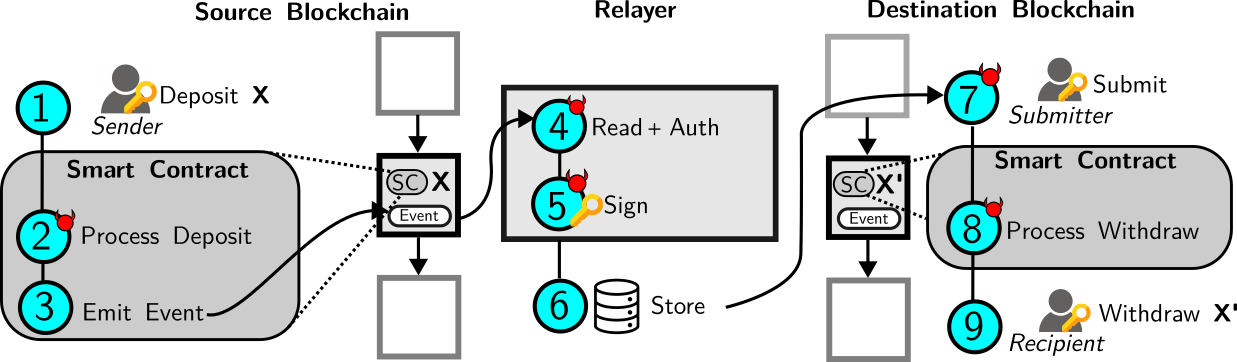
\includegraphics[width=0.8\textwidth]{fig/bridge_arch.pdf}
%%command for cropping pdf
%%gs -sDevice=pdfwrite -o bridge_arch_crop.pdf bridge_arch.pdf
\caption{Cross-chain token bridging and the different steps attackers can exploit to withdraw unbacked deposits.}
\label{fig:cross-chain}
\end{figure*}

\section{Background}
\label{sec:background}
% In this section, we start by providing an overview of blockchain technology. We then describe how cross-chain bridges work followed by the threat model we consider in this paper.
% In this section
We first give a brief introduction to smart contract blockchains
and cross-chain bridges. We then describe how bridges, under attack, collapse in
practice.

\subsection{Smart-contract Blockchains} Modern DeFi protocols (e.g.,
decentralized exchanges and lending protocols) are built on top
of ``smart-contract'' blockchains, like Ethereum. At their core, these chains, like
the original Bitcoin blockchain, are distributed ledgers that manage accounts
(public keys) and their balances (in native tokens like Ethereum's ETH). Users
interact with these chains by signing and broadcasting (to the distributed nodes
that make up the chain network) transactions that, for example, transfer
funds from their account (using the corresponding account private key) to
another user's account.

Ethereum, and the smart-contract chains it inspired since its release in 2015,
differ from Bitcoin by extending the ``simple'' distributed ledger with a smart
contract execution layer. A smart contract on Ethereum is an \emph{internal}
account---and, like a normal, \emph{externally owned} account (EOA), it has a
balance---that has associated \emph{code} (EVM bytecode), which implements the
smart contract's program logic, and \emph{storage}, which persists the program's
state across executions. Users interact with (i.e., execute) smart contracts
much like they do when transferring funds from their account: they sign a
transaction that encodes the smart contract to call (i.e., the contract address),
the particular function to execute, and the arguments to call the function with.
Instead of simply transferring funds from the user's account, then, executing
such a \emph{smart-contract call} transaction amounts to executing the smart
contract bytecode---and any smart contracts the contract itself calls.
    
% \begin{lstlisting}
% contract USDC{
%   mapping(account => amount) _balances;
%   event Transfer(from, to, value);
%   function transfer(to, amount) {
%     address from = msg.sender; // user
%     // ... validate user has enough balance
%     _balances[from] -= amount;
%     _balances[to] += amount;
%     emit Transfer(from, to, amount);
%   }

%   function mint(to, amount) {
%     _balances[to] += value;
%     emit Transfer(address(0), to, amount);
%   }

%   function burn(from, amount) {
%     // ... validate user has enough balance
%     _balances[from] -= amount;
%     emit Transfer(from, address(0), amount);
%   }

%   function safeTransferFrom(from, to, amount){ 
%     // ... transfer tokens; revert if failed
%   }
% }
% \end{lstlisting}


\begin{figure}[t]
    \centering
    \includegraphics[width=\columnwidth]{fig/usdc-contract-2sp.pdf}
    \caption{Simplified USDC ERC-20 Token Contract.}
    \label{fig:erc20}
\end{figure}


    

% \lstdefinestyle{myStyle}{
%     belowcaptionskip=1\baselineskip,
%     breaklines=true,
%     % frame=none,
%     % numbers=none, 
%     basicstyle=\footnotesize\ttfamily,
%     % keywordstyle=\bfseries\color{green!40!black},
%     % commentstyle=\itshape\color{purple!40!black},
%     % identifierstyle=\color{blue},
%     backgroundcolor=\color{gray!10!white},
%     language=Python,
% }

% \lstdefinestyle{customc}{
%   belowcaptionskip=1\baselineskip,
%   breaklines=true,
%   frame=L,
%   xleftmargin=\parindent,
%   language=Python,
%   showstringspaces=false,
%   basicstyle=\footnotesize\ttfamily,
%   keywordstyle=\bfseries\color{green!40!black},
%   commentstyle=\itshape\color{purple!40!black},
%   identifierstyle=\color{blue},
%   stringstyle=\color{orange},
% }


\subsection{ERC-20 Tokens}
One of the immediate applications of smart contracts---and to date still one of
most popular---is to create custom tokens (or coins).  To launch a new token, an
organization no longer needs to launch a new blockchain; they can instead deploy
a new contract that implements the ERC-20 token standard interface on a chain
like Ethereum and take advantage of existing on-chain infrastructure like
decentralized exchanges that make it easy to, for example, trade one kind of
token for another---both native tokens (e.g., ETH) and other tokens.\footnote{
    Most EVM chains, i.e., chains that use Ethereum's execution layer,
    follow Ethereum standards like ERC-20. Most non-EVM chains like Solana
    (which have different execution models) have similar standards (e.g., SPL
    tokens in Solana's case).
}

Figure~\ref{fig:erc20} shows a simplified variant of one such token
contract---the USDC \emph{stablecoin} contract.  This contract tracks
how many USDC tokens an account has and governs the spending of these
tokens (much like a bank governs bank notes).  For example, the
contract's \texttt{mint} function lets Circle (the company that owns
the USDC contract) mint new tokens into a user's account---e.g., after
receiving the corresponding payment from the user off-chain (in US
dollars, as USDC tokens are pegged to the US dollar).  The contract
exposes the ERC-20 interface that lets users (and smart contracts)
transfer tokens from their account by simply calling functions like
\texttt{safeTransferFrom}, and, in turn, use the tokens in any DeFi
protocol (e.g., lending the USDC to different markets, exchanging USDC
for ETH,
% buying NFTs using the USDC,
etc.). Finally, the contract's
\texttt{burn} function ``burns'' a token out of circulation---and
emits an event (Figure~\ref{fig:erc20-event}) that Circle's off-chain code looks for before allowing
a user to withdraw the corresponding USD fiat off-chain.

% \subsection{Blockchain Basics}
% In this section, we cover the basic concepts of blockchain technology, including blockchains, smart contracts, transactions, accounts, and tokens.

% \textbf{Blockchains.} A blockchain is a distributed ledger that stores data (e.g., account balance) in a transparent and tamper-proof manner. It consists of a chain of blocks, where each block contains a certain amount of data, a reference to the previous block (thus forming a chain), and other information such as timestamp. Blockchains are maintained by a network of nodes that validate data in the blocks and reach consensus on the state of the ledger.\alex{somehow have to mention Solana and Ethereum and others?}
% % It consists of a series of blocks that are linked together via cryptography (thus forming a chain) [65]. These blocks are immutable and can be used to store data (e.g., transactions). They are also maintained by a distributed network of nodes, removing the need of a central server. 

% \textbf{Smart Contracts.} Smart contracts are programs that can be executed. Typically, smart contracts are first written in high-level programming languages such as Solidity or Rust. Then, they are compiled into bytecode and deployed to the blockchain. Upon deployment, each smart contract is assigned a unique address and becomes immutable. After deployment, they can be executed based on the input provided and the logic programmed into the contract.

% % , compiled into bytecode, and deployed to the blockchain. The input and execution of smart contracts are all recorded on the blockchain. They 

% % are stored and executed on blockchains. They are used to encode business logic, enforce rules, and automate processes. Smart contracts are written in high-level programming languages, compiled into bytecode, and deployed to the blockchain. Once deployed, smart contracts are immutable and can be interacted with by sending transactions.

% % self-executing programs that run on blockchains. They are used to encode business logic, enforce rules, and automate processes. Smart contracts are written in high-level programming languages, compiled into bytecode, and deployed to the blockchain. Once deployed, smart contracts are immutable and can be interacted with by sending transactions.

% \textbf{External Owned Accounts.}  Externally owned accounts (EOAs) represent users and are controlled by private keys. Users can interact with other users or deployed smart contracts by initiating a transaction from their EOAs. To initiate a transaction, a user specifies the recipient (the address of an EOA or a smart contract), the amount of assets to transfer, and any additional input parameters required by the smart contract. 

% % are entities that can send and receive transactions on the blockchain. There are two types of accounts: externally owned accounts (EOAs) and contract accounts. EOAs are controlled by private keys and represent human users, while contract accounts are controlled by smart contracts and represent autonomous entities.

% % Accounts are entities that can send and receive transactions on the blockchain. There are two types of accounts: externally owned accounts (EOAs) and contract accounts. EOAs are controlled by private keys and represent human users, while contract accounts are controlled by smart contracts and represent autonomous entities.


% \textbf{Transactions.} A transaction is a instruction set constructed and signed by a user using their EOA. It typically includes several fields, such as the sender (the EOA that signs the transaction), the recipient (which can be an EOA or a smart contract), the amount of assets to transfer, and the input parameters required by a smart contract. Once signed, the transaction is broadcasted to the network and executed. After successful execution, the resulting state changes are recorded on the blockchain along with the transaction itself.


% \textbf{Tokens.} Every blockchain system has its own native token. For example, Ethereum has Ether (ETH), while Solana has Sol (SOL). In addition to native tokens, blockchains can also host other types of tokens. An example is ERC-20 tokens on Ethereum, which are smart contracts that follow a set of rules and standards. Of particular note, when a user transfers ERC-20 tokens, the ERC-20 token contract emits an event (a type of debug information recorded on the blockchain) that logs certain information. Figure 1 shows an example. The name of the event is Transfer, and the token contract that emits the Transfer event is tagged as USDC. The sender and recipient are represented by their addresses (0x68... and 0xF5..., respectively). The amount of tokens transferred is 212295874.

% \alex{maybe liquidity pool}


\subsection{Cross-Chain Token Bridges}
While smart contracts make it easy to launch new tokens without spinning up new
chains, there is no real shortage of new blockchains being deployed (almost weekly).  Indeed,
the modern blockchain ecosystem is a many-chain ecosystem.  Blockchains like
Avalanche, Base, and Solana have different design points---from cheaper ``gas''
execution costs, to higher throughput, lower latency, and different permission
models---that make them better suited for different classes of application.
This situation has resulted in applications that span many chains and cross-chain
infrastructure that ultimately (try to) allow users to, for example, buy
Dogwifhat NFTs on Solana using USDC tokens on Ethereum.

Core to these applications and infrastructure---and the focus of our work---is
the \emph{cross-chain token bridge}.  At a high level, a cross-chain token
bridge makes it possible for a user to ``transfer'' their tokens from one chain
(e.g., their USDC on Ethereum) to another chain (e.g., Solana) and then use the
transferred tokens on the destination chain (e.g., on a Solana exchange trading
USDC and Dogwifhat).\footnote{While some cross-chain bridges \emph{do} let users
transfer one kind of token (e.g., USDC on Ethereum) for a completely different
kind of token on the destination chain (e.g., Dogwifhat on Solana), these bridges
essentially fuse the cross-chain token bridge with an exchange (or swap). We
focus on token bridges not only because they are fundamental to other kinds of
bridges, but also because they have higher volume, more liquidity, and more
attacks.} Since smart contracts cannot make network requests or otherwise
access sate outside their own storage, a cross-chain token bridge consists of
smart contracts on both the source and destination chains, and off-chain
infrastructure that serves to relay the ``transfer'' call across the two
contracts.

\begin{figure}[t]
\centering
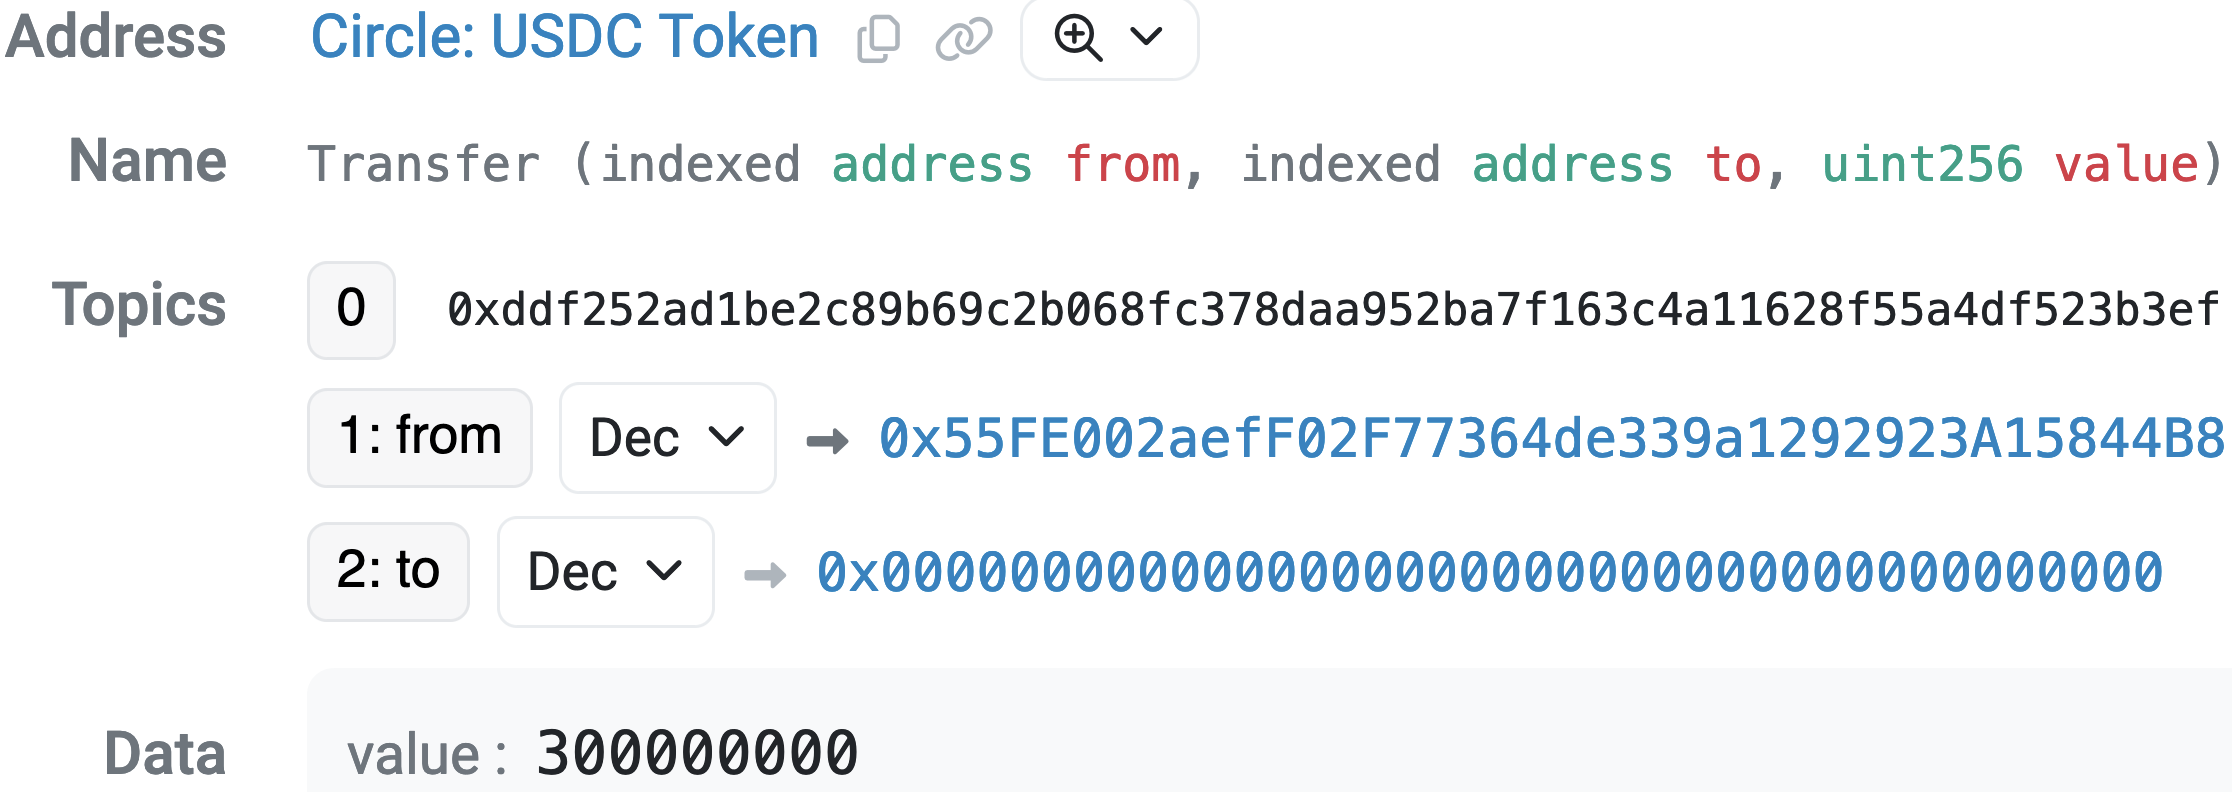
\includegraphics[width=\columnwidth]{fig/token.png}
\caption{Event Emitted by an ERC-20 Token (USDC).}
\label{fig:erc20-event}
\end{figure}

As Figure~\ref{fig:cross-chain} shows, a typical cross-chain token transfer,
i.e., a bridge transaction, consists three phases:

\textbf{1. Deposit (on source chain).}
To initiate a cross-chain token transfer, the user first calls the bridge's
contract on the source chain:
\begin{lstlisting}
deposit(address token, uint256 val, address to) {
  address from = msg.sender;  // user
  address to = address(this); // bridge contract
  // ... validate the ERC-20 token contract
  token.safeTransferFrom(from, to, val);
  emit Deposited(id++, token, from, to, val);
}
\end{lstlisting}
This contract function---a simplified version of the Qubit bridge deposit
function---processes the user's deposit (step 2) by validating the transfer request,
e.g., against a list supported tokens, and then transferring the user's ERC-20
tokens to the bridge contract---recall contracts are accounts with balances.
Then, the function emits an event (step 3) recording the user's deposit details
(including the deposit ID, the ERC-20 token contract address, the recipient on
the destination chain, and value).

\textbf{2. Off-chain relay.}
The emitted event is observed by an off-chain relayer in (step 4),
which constantly monitors the source blockchain.  The relayer first
verifies the authenticity of the deposit event.  If the event is
authentic, the relayer then produces a signed \emph{receipt}
endorsing the deposit (step 5) and, typically, stores the receipt off-chain (step
6).  Finally, this signed receipt is sent to the bridge's withdrawal contract
on the destination blockchain (step 7). Who submits the receipt varies across
bridges---some bridges submit the receipt on the user's behalf (in these cases, the
signed receipt is simply a signed contract-call transaction), while others give
users (and anyone willing to pay gas) the signed receipt and they, in turn,
submit the receipt to the withdrawal contract to complete the transfer. 

\textbf{3. Withdraw (on destination chain).}
The withdrawal contract on the destination chain first processes the withdraw
request by verifying the receipt and transferring the tokens to the recipient
(step 8). In (the simplified) Chainswap's withdraw case, for example, users call:
\begin{lstlisting}
withdraw(uint256 id, address token, address to, uint256 val, Signature[] sigs) {
  _chargeFee();
  // verify receipt
  require(received[id][to] == 0, 'withdrawn');
  for(uint i=0; i < sigs.length; i++) {
    verify_receipt(sigs[i], id, token, to, val);
  }
  received[id][to] = val; // mark as withdrawn
  token.safeTransferFrom(address(this), to, val);
  emit Withdraw(id, token, to, val);
}
\end{lstlisting}
This contract function first charges the caller a fee, then verifies the
deposit details against receipt---both that the deposit was not already
withdrawn and that the receipt signatures are valid---and finally transfers the
tokens to the intended recipient.  We consider a cross-chain transaction
complete when the asset is released to the recipient (step~9).

We expect every cross-chain bridge transaction to uphold the balance invariant:
the value (and kind) of the tokens withdrawn---the outflow---should equal the
value (and kind) of the tokens deposited---the inflow---minus the charged fees.
In practice, they do not.



% \subsection{Cross-Chain Bridges}
% In this section, we begin by providing an example of how a typical cross-chain transaction works. We then discuss the different variants of cross-chain bridges. 
% \subsubsection{A Typical Cross-Chain Transaction}
% Figure~\ref{fig:cross-chain} depicts a typical cross-chain transaction. Starting with the source blockchain, the sender (represented by their EOA) initiates a transaction to transfer assets to the bridge's deposit contract (step 1). The bridge contract then verifies that it has received the assets (step 2). Upon verification, the bridge contract emits an event to record the transfer (step 3). This event is observed by the relaying component (step 4), which typically resides outside and constantly monitors the source blockchain. The relaying component then verifies the authenticity of the event (step 5). If the event is authentic, the relaying component signs the message and stores the signature in a queryable database (step 6). A submitter on the destination blockchain then fetches the signed message from the database (step 7) and sends it to the bridge's withdrawal contract on the destination blockchain (step 8). The bridge contract then verifies the signature (step 9) and transfers the assets to the recipient (step 10). A cross-chain transaction is considered complete when the asset is released to the recipient (step 11).

% % Important things we need in this figure:
%     % source and dst amount
%     % how different vulnerabilities manifest
%         % source
%             % transfer in
%             % verify * emit
%         % relaying component
%             % observe
%             % signs
%         % dst
%             % retrieve & send
%             % verify
%             % transfer out
%     % Players
%         % Sender (in source)
%         % Relayer (in dst)
%         % Receiver (in dst)
    
    



% \subsubsection{Variants of Bridge Implementation}
% Beyond the typical cross-chain transaction described above, there are different ways to implement a cross-chain bridge. We discuss the following variants:

% \textbf{Asset Management.} There are two common ways funds can be released in step 10. The first model is the liquidity pool, which is commonly used when an asset already exists on both blockchains (e.g., USDC already exists on Ethereum and Polygon). Bridges start by creating liquidity pools, to which users can deposit assets and earn fees. When a withdrawal request is made, the bridge releases the funds from the liquidity pool as long as there is sufficient capital in the pool. The second model is mint-and-burn, which can be used regardless of whether the asset exists on the destination blockchain. In this model, the bridge contract mints new tokens on the destination blockchain, which act as representations of the assets on the source blockchain. When a withdrawal request is made, the bridge simply mints new tokens and sends them to the recipient. The recipient can then burn the tokens to receive the original assets on the source blockchain.



% \textbf{Submitter Privilege.} In the flow depicted in Figure~\ref{fig:cross-chain}, once the relaying component has signed the transaction, anyone can fetch the signed message and submit it to the destination blockchain. However, in practice, there is a variant where only privileged EOAs can act as submitters. In this variant, the authenticity of the message is verified by the presence of a privileged key. If bridges choose to operate in this way, they 
% typically simplify step 6 by directly storing the message without signing it.

% \textbf{Transaction Relay.} In the flow depicted in Figure~\ref{fig:cross-chain}, each transaction is relayed individually. In practice, transactions can also be relayed in batches or grouped into a Merkle tree. This approach can improve efficiency. However, while using a Merkle tree is more efficient, it also introduces additional complexity in step 9, where the bridge contract has to verify that a transaction is included in a Merkle tree.

% \textbf{Message Verification Mechanisms.} There are four different mechanisms to verify the authenticity of a message. Namely, external verification, optimistic verification, native verification, and local verification. The details of these mechanisms are not critical for this paper. We provide a brief overview of each model and refer the reader to \alex{cite} for more details. At a high level, external verification indicates that the relaying component resides outside both the source and destination blockchains. The legitimacy of a cross-chain transaction is attested by a third party (or a set of third parties). Native verification, on the other hand, indicates that the relaying component resides within the destination blockchain. In this model, the relaying component typically operates as a light client of the source blockchain and maintains enough information to verify the authenticity of a message from the source blockchain. Optimistic verification improves the efficiency of external verification by assuming that the majority of relayed transactions on the destination blockchain are valid. Instead of attesting to the validity of every transaction, optimistic verification only intervenes when a fraudulent transaction is detected. Finally, local verification means that the two parties involved in a cross-chain transaction (e.g., the sender and the submitter) must cooperate and collaborate for the transaction to succeed.

% \textbf{Token Swap Bridges.} In the above example, tokens released on the destination blockchain are backed by an equivalent amount of assets (less fee) on the source blockchain. However, in practice, bridges can also support token swap. In this case, an asset on the source blockchain is swapped for a different asset on the destination blockchain. For example, a user can swap 1 ETH for 100 USDC. The conversion rate is typically determined by the relaying component and may not be publicly disclosed. 

% \subsubsection{Variants of Verification Mechanism.}
% \textbf{External Verification.} In the most common case, the verification components resides outside both the source and destination blockchains. This is known as an externally verified bridge. The legitimacy and correctness of a cross-chain transaction is determined by a third-party (or a set of third-parties). Common ways to implement external verification include Multi-party Computation and Threshold Signature Scheme.\alex{cite}

% \textbf{Optimistic Verification.} Optimistic Verification improves on the efficiency of external verification by assuming that the majority of transactions are valid. Instead of attesting to the validity of every transaction, optimistic verification only intervenes when a dispute arises. This is known as an optimistic bridge. Concretely, every message that is passed to the destination blockchain is considered "pending" until the dispute window expires. The system relies on one or more honest watchers to dispute the message if it is incorrect. If no dispute arises, the message is considered valid.

% \textbf{Native Verification}
% Contrary to external verification, where the verification component resides outside the source and destination blockchains, the verification component in a natively verified bridge resides within the destination blockchain. Commonly, this is achieved by implementing a light client of the source blockchain within the destination blockchain, which maintains enough information for verifying the authenticity of a message. The security is guaranteed by the validators of the source chain. 


% \textbf{Local Verification}
% \alex{add citation. this is the most confusing one.}
% The basic idea is that the sender and the submitter
% have to cooperate and collaborate for a cross-chain transaction to succeed. 

\subsection{How Bridges Collapse}
In practice, attackers exploited bugs in all three components---the deposit
contract, the relayer, and the withdraw contract---and stole signing keys
to siphon hundreds of thousands of dollars.
%
Figure~\ref{fig:cross-chain} highlights the precise steps in the cross-chain
token transfer that attackers have historically exploited, including:
\begin{CompactItemize}
\item \textbf{Bugs in the deposit contract.} In step 2, the bridge contract
verifies that it has received the correct amount of assets before emitting an
event. Bugs in this verification logic could allow an attacker to deposit a
smaller amount of assets than what is recorded by the bridge in the event (step
3). For example, Qubit's \texttt{deposit} function  (see above) did not properly validate the token address. This bug allowed an attacker to pass \texttt{0} for the token address, so the contract function did not actually transfer any funds from the attacker's account but still emitted a \texttt{Deposit} event which allowed the attacker to withdraw actual tokens on the destination chain~\cite{qubit:rekt}.

\item \textbf{Bugs in the off-chain deposit verification.} In step 5, the
relayer verifies the authenticity of the deposit event emitted by the
bridge contract, including whether the event is emitted by the bridge's
designated contract.  Bridges that do not correctly verify
deposits would allow attackers to withdraw assets that are never deposited.
% ---and this 

\item \textbf{Stolen relayer (or submitter) keys.} In step 5, the relayer signs the deposit receipts which are then submitted to the withdrawal
contract as evidence of a valid deposit. If the relayer key is compromised
(e.g., as with the Ronin bridge~\cite{roninattack}) the attacker can forge a
valid receipt and then withdraw assets that were never deposited by calling
\texttt{withdraw} with the forged receipt.

The same is true for bridges that submit receipts on behalf of users---and
essentially restrict the \texttt{withdraw} callers to privileged submitter
accounts. The bridge submitter keys (step 8) have similarly been compromised
(e.g., as with AnySwap~\cite{anyswapattack}) and used to withdraw
unbacked deposits.

\item \textbf{Bugs in the withdraw verification.} In step 8, the bridge contract
verifies that the messages are signed by the relayer and have not
been replayed. Bugs in this verification logic (e.g., as we saw with
Wormhole~\cite{wormholeattack}) have allowed attackers to supply ``valid''
payloads that were not signed by the relayer and replay withdrawal
requests with valid deposit receipts that have already been withdrawn.
\end{CompactItemize}


% Liquidity Pool vs Mint-and-Burn. Example USDC on ETH and Polygon
% Verification Modes
% \subsection{Threat Model}
% In this section, we describe the attack surfaces that are in scope for this paper. Importantly, we assume that deposits and withdrawals are made through designated functions and that funds cannot be withdrawn through functions other than the designated withdrawal function(s). Given this setup, we consider the following attack surfaces:

% \textbf{Buggy Deposit Verification.} In step 2, the bridge contract verifies that it has received the correct amount of assets before emitting an event. Bugs in this verification logic could allow an attacker to deposit a smaller amount of assets than what is recorded by the bridge in the event (step 3).

% \textbf{Buggy Event Verification.} In step 5, the relaying component verifies the authenticity of the event emitted by the bridge contract, including whether the event is emitted by the bridge's designated contract. Failure to do so could allow an attacker to withdraw assets that were never deposited.

% \textbf{Compromised Relaying Key.} In step 6, the relaying component signs the message and stores the signature in a queryable database. If the relaying key is compromised, an attacker could forge a message and withdraw assets that were never deposited.

% \textbf{Compromised Submitter Key.} In step 8, some bridges operate in a privileged submitter mode, where the presence of the privileged submitter key is the only requirement to attest to the authenticity of a message. In this case, if the submitter key is compromised, an attacker could submit a forged message and withdraw assets that were never deposited.

%\textbf{Buggy Withdraw Verification.} In step 9, the bridge contract verifies that the messages are signed by the relaying component and have not been replayed. Bugs in this verification logic could allow an attacker to verify payloads that are not signed by the relaying component or to replay a message that has already been processed.

In this paper, we assume an attacker can exploit any of the aforementioned
components or otherwise control the relayer (or submitter) keys.
In the next section, we show that this attacker model and our simple
\emph{balance invariant checking} captures the largest attacks on cross-chain
bridges that have happened in the past.  In Sections~\ref{sec:live-audit} we show
that monitoring withdrawals and deposits on the source and destination chains
can be used to detect similar attacks in the future.  Finally, in
Section~\ref{sec:active-protect} we describe an \emph{announce-then-execute} bridge
design that enforces this invariant to prevent attacks before they happen.

We note that while our threat model captures a wide variety of vulnerabilities,
it is not exhaustive.  As with any detection system, an attack that violates one
of our assumptions (e.g., avoids violating the balance invariant by transferring
funds off-bridge or not having a withdrawal, subverts the transaction data used to validate the invariant,
etc.) might succeed.  
We similarly consider other smart contract bugs (beyond bugs in deposit and withdrawal functions) and account key compromises out of scope---and instead focus
on the cross-chain bridging aspects which are relatively less well understood.
As we show later, our model captures the largest attacks on
cross-chain bridges that have happened in the past and systems can use
it to prevent similar attacks in the future.


%% While our approach captures a variety of vulnerabilities, it is by no
%% means exhaustive. For example, a key assumption we make is that
%% withdrawal are done through designated withdraw functions. However, if
%% an adversary is able to compromise the key to account that holds the
%% funds for the bridge, they could simply transfer the funds to another
%% account and then withdraw them without going through the designated
%% withdraw function(s). Similarly, if an adversary is able to withdraw
%% funds by repurposing other functions (e.g., the deposit function), our
%% approach would not detect it. Moreover, if an attack transaction does
%% not involve a withdrawal, our approach would not detect it. Last but
%% not least, if an attack is somehow able to profit without breaking the
%% balance invariant, our approach would not detect it.  However, we
%% believe that our approach is a important first step in using
%% accounting principles to protect bridges from theft and that it can be
%% extended to address these and other vulnerabilities in the future.


\section{Approach}
\label{sec:meth}

The core hypothesis of our work is that value should be conserved
within cross-chain transactions.  That is, that the value of the asset
inflow in such a transaction (i.e., the deposit) should equal the
value of the asset outflow (i.e., the withdrawal).  In token transfer
bridges, this invariant corresponds to a balancing of the inflow
tokens and the outflow tokens (less any fees or transaction costs
incurred by the bridge itself).  When this balance invariant does not
hold it allows a range of opportunities for fraud, all of which
involve greater outflows (withdrawals) than inflow
(deposits). Figure~\ref{fig:invariant} illustrates such an outcome by 
graphing the \emph{aggregate} difference between bridge inflow (on
Ethereum) and outflow (on Solana) leading up to and during the
February 2022 attack on the Wormhole bridge.  The net difference is
consistently near zero, with only short positive deviations
(representing delayed withdrawals) until the attack in January, at
which point there are significant withdrawals without matching
deposits---producing a large negative difference.

Testing this invariant on a \emph{per transaction basis} is
straightforward in principle. However, since bridge transaction formats are
not standardized, it requires a range of per-bridge and per-chain
parsing in practice.  Our methodology for normalizing this information
focuses on two key pieces of information: a) identifying each bridge
transaction---a composite of a deposit (inflow) transaction on a
source blockchain and a withdrawal (outflow) transaction on
another---and b) identifying the value transferred in each such bridge
transaction.

\begin{figure}[t]
  \centering
  \includegraphics[width=0.7\columnwidth]{fig/sec25_plot_wormhole.pdf}
  \caption{Total Inflow (on Ethereum) - Total Outflow (on Solana) Over Time: Wormhole Attack in Feb 2022.}
  \label{fig:invariant}

\end{figure}


\subsection{Identifying Bridge Transactions}
For almost all bridges, identifying their component (per-chain) inflow
and outflow transactions is straightforward --- bridges typically use
explicit events on each chain to signal if a given transaction is a
deposit or withdrawal.\footnote{One key exception to this rule is the
  Wormhole bridge which, until late 2023, did not emit specific
  events when executing a withdrawal transaction.  In this case, we infer that a withdrawal took
  place by looking for transactions that invoke functions designated for performing withdrawal operations (e.g., \textit{completeTransfer}).
  %have synthesized such an event ourselves by parsing the function
  % names called by the transaction to .  
  It also appears to be widely understood today that emitting
  explicit events is a best practice.}

Pairing these component transactions (i.e., matching deposits on one
chain to withdrawals on other) can be performed in several different
ways.  The easiest, and most common, is via a unique transaction
identifier. Such IDs are typically generated by the bridge on the
\emph{source chain} during a deposit transaction and then copied into
the withdrawal transaction on the destination chain.\footnote{These
  unique IDs are commonly simple global variables incremented with
  each new transaction.}  However, instead of an explicit ID, some
bridges use a hash of the deposit transaction for the same purpose
(e.g., for Anyswap, each withdraw transaction will include the hash of
its corresponding deposit transaction).\footnote{We note that to prevent potential replay attacks, bridge implementers should also include an ID that uniquely identifies individual deposit events within a transactions. Sadly, this is often not the case.}  Finally, in a handful of cases there are
no ``inband'' identifiers that can be used to associate transactions.
We believe this is a poor design choice that is fundamentally in
conflict with auditability.  However, even in these cases, for the
purpose of our analysis we have been able to pair transactions using
explicit query APIs provided by the affected bridges
services.\footnote{For example, when a bridge transaction on the Poly
  Network bridge includes a withdrawal from Curve (a kind of liquidity
  pool) or when a bridge transaction on the Binance Token Hub includes
  a Binance Smart Chain (BSC) withdrawal, it is not possible to
  identify the partner deposit from blockchain data alone and we must
  make use of ``out of band'' data available through their respective
  bridge query APIs.}

  At the end of this process, we identify a comprehensive collection
  of ``bridge transactions'' (a pair of transactions from two
  different blockchains that were used by the bridge to transfer
  value across them). While the vast majority of bridge transactions
  are pairs of deposit and withdrawal transactions, a handful of
  bridge transactions are either withdrawal-only (e.g., in the case of
  attacks) or deposit-only (e.g., if the user chooses to delay their
  withdrawal).

% And for 
% a handful of bridge transaction, they are either withdrawal-only or deposit-only, and we treat them as singleton transactions.
%  and a handful of singleton
% transactions (i.e., which involve the bridge, based on their
% addresses, but are withdrawal-only or deposit-only).


%For example, with the Binance bridge, the matching transaction for a BSC transaction can only be identified by querying the API. 
%%% here.
%Similarly, for Poly Network bridge, when users withdraw from Curve (a kind of liquidity pool), the matching deposit amount is not recorded on the blockchain, as its a special type of withdrawal where the matching deposit is computed off-chain and only available through the API. In this case, we also rely on Poly Network's API to pair the deposit and withdraw transactions, if the deposit transaction is from Curve. \elisa{It might be nice to give a reason why the pairing info is not available for these cases if we know.} 




%\textbf{Using Unique ID.} Most of the bridges\alex{how many?} will create a unique id for each deposit transaction (incrementing by 1).
%A withdraw transaction will contain this unique id. We can then use this unique id to pair the deposit and withdraw transactions.



%\textbf{Using the transaction hash of the deposit transaction.}
%Another way to pair deposit and withdraw transactions is to use the transaction hash of the deposit transaction. A withdraw transaction will include the transaction hash of the corresponding deposit transaction hash. We can then use this information to pair the deposit and withdraw transactions.

%\textbf{Using the official API.}
%Some bridges provide APIs to query matching deposit and withdraw transactions. While this feature mostly exist for user convenience, sometimes we have to rely on this API to pair deposit and withdraw transactions, as the pairing information is not directly available as part of the withdraw transaction.\alex{maybe we should hedge here and say its not trivial to get the information.} 
%For example, with the Binance bridge, the matching transaction for a BSC transaction can only be identified by querying the API. 
%%% here.
%Similarly, for Poly Network bridge, when users withdraw from Curve (a kind of liquidity pool), the matching deposit amount is not recorded on the blockchain, as its a special type of withdrawal where the matching deposit is computed off-chain and only available through the API. In this case, we also rely on Poly Network's API to pair the deposit and withdraw transactions, if the deposit transaction is from Curve. \elisa{It might be nice to give a reason why the pairing info is not available for these cases if we know.} 

\subsection{Identifying the Value Transferred}
Many bridge transaction event formats explicitly identify the amount
and kind of tokens transferred. However, some bridges do not emit this
information and others can be unreliable.\footnote{For example, as
  mentioned earlier, pre-2024 Wormhole does not emit an event for
  withdrawal transactions. Other examples include the Meter bridge and
  Qubit bridge, which attempted to verify the number of tokens
  received but had exploitable bugs.}  In such cases, we can
frequently make use of the ERC-20 ``Transfer'' event (see
Figure~\ref{fig:erc20-event} for an example) that is emitted when the
contract transfers the tokens from the user's account to the bridge's
account.  This event contains the number of tokens transferred as well
as the sender and recipient addresses, which we use to identify the
number of tokens transferred to or from the bridge.  Because the
Transfer event is adjacent to its associated bridge-generated event,
it is easy to identify and thus establish the number of tokens
transferred.\footnote{As a sanity check, we also require that the
  sender and recipient addresses in the Transfer event are consistent
  with the bridge's defined behavior: for withdrawal transactions, we
  require that the sender is either a mint address (i.e., all-zero
  address) or a bridge-controlled address, while for deposit
  transactions, we require that the recipient is either a burn address
  (i.e., all-zero address) or a bridge-controlled address.}  In a few
implementations, multiple related Transfer events can be emitted at
once, and in these cases we have manually inspected their contracts
and constructed implementation-specific logic to account for this
behavior.  Another special case is caused by so-called ``reflection
tokens'' in which the number of tokens logged in the event (the value
field in Figure~\ref{fig:erc20-event}) is dynamically adjusted based
on a combination of the intended number and the total token supply.
For such cases, we either rely on bridge events which capture the
intended number of tokens transferred or implement token-specific
logic to recompute the value accordingly.  Finally, native tokens have
no Transfer event (since they are not ERC-20 tokens), but thus far we
have either been able to recover the number of tokens transferred from
bridge events or so-called ``internal transactions''.

To summarize, while it is certainly possible to create a bridge
transaction protocol that records insufficient data to match deposits
and withdrawals, or for which the number of tokens transferred might
be ambiguous, our empirical experience analyzing 11 bridges and 21
blockchains is that such reconstruction has always been possible.


%When the amount of tokens transferred logged by the bridge is unavailable or unreliable, we can use the Transfer event emitted by an ERC20 token contract to identify the amount of tokens transferred. The Transfer event, part of the ERC20 standard, has been used by prior research in other scenarios.\alex{cite} This event contains the amount of tokens transferred as well as the sender and recipient addresses, which we use to identify the amount of tokens transferred to or from the bridge. Concretely, we observe that for any successful bridge transaction, depending on the order of execution, the transfer event either happens right before or after the bridge-generated event. As a result, we can first locate the bridge event and then look for the Transfer event that happens right before or after the bridge event, which contains the amount of tokens transferred. As additional sanity checks, we also require that the sender and recipient addresses in the Transfer event are consistent with the bridge's behavior. Namely, for withdraw transactions, we require that the sender is either a mint address (e.g., all-zero address) or a bridge controlled address. On the other hand, for deposit transactions, we require that the recipient is either a burn address (e.g., all-zero address) or a bridge controlled address.\alex{do we have to explain the intuition?}


%There are two ways to identify the amount of tokens transferred by the bridge: using the amount logged in a 
%bridge-generated event or using the Transfer event emitted by ERC20 tokens. Specifically, some bridges include the amount of tokens sent or received in their events. However, this information is not always reliable, as bridges can have bugs (typically when they don't verify the amount of tokens they actually received), which is the case for [AL: which]. Additionally, some bridges do not emit this information. In such cases, we can use the token transfer event to identify the amount of tokens transferred, which also serves as the ground truth.

%\textbf{Identifying Token Transferred from Transfer Event.} 
%When the amount of tokens transferred logged by the bridge is unavailable or unreliable, we can use the Transfer event emitted by an ERC20 token contract to identify the amount of tokens transferred. The Transfer event, part of the ERC20 standard, has been used by prior research in other scenarios.\alex{cite} This event contains the amount of tokens transferred as well as the sender and recipient addresses, which we use to identify the amount of tokens transferred to or from the bridge. Concretely, we observe that for any successful bridge transaction, depending on the order of execution, the transfer event either happens right before or after the bridge-generated event. As a result, we can first locate the bridge event and then look for the Transfer event that happens right before or after the bridge event, which contains the amount of tokens transferred. As additional sanity checks, we also require that the sender and recipient addresses in the Transfer event are consistent with the bridge's behavior. Namely, for withdraw transactions, we require that the sender is either a mint address (e.g., all-zero address) or a bridge controlled address. On the other hand, for deposit transactions, we require that the recipient is either a burn address (e.g., all-zero address) or a bridge controlled address.\alex{do we have to explain the intuition?}

%\textbf{Additional Considerations.}
%We note a few additional considerations. First, while the transfer action usually results in a single event, there are cases where multiple Transfer events are emitted. In such cases, we need to incorporate token-specific logic to capture a series of Transfer events to identify the amount of tokens transferred. For tokens exhibiting this behavior, we manually examine their code and account for their logic in our analysis.
%Next, for transfers involving native tokens, the value sometimes is included in internal transactions, and no event is emitted. We use the internal transactions to identify the amount of tokens transferred. Lastly, for a special type of tokens called reflection tokens, we need to account for the reflection mechanism. Specifically, reflection tokens have a mechanism where the real amount of tokens transferred is dynamically adjusted based on intended amount and total supply. For some tokens, they emit events that include enough information to recompute the intended amount. We thus use this information to identify the intended amount of tokens transferred. For other tokens, they do not provide such information. However, for those cases, conveniently, the bridge event includes the intended amount of tokens transferred. We thus revert back to use the amount logged by the bridge.\footnote{The delta between the intended amount and the real amount is very small (typically within a factor of 0.01). Thus, even if the initial amount is not logged by the bridge, the intended amount can still be bounded.}

\subsection{Checking the Balance Invariant}
Once we have identified both sides of the bridge transaction and the
number of tokens transferred by the bridge, we can verify if the
balance invariant holds: for each bridge transaction (including those
that are withdrawal-only), does the number of tokens transferred from
the bridge---the withdrawal amount---match the number of tokens
received by the bridge---the deposit amount?

However, a key complication is that bridges can charge fees and, while
these fees can sometimes be paid ``out of band'', it is not uncommon
for them to be subtracted from the tokens received on deposit.  To
account for this behavior (i.e., outflow = inflow - costs), we must be
able to determine such costs on a per-transaction basis.
In most cases, fees can be accounted for in a straightforward manner:
they either are made explicit in bridge-generated events (and can thus
be accounted for directly) or can be calculated based on either
published fee schedules or inferred fee schedules (i.e., since all
transactions are typically subject to the same fixed or percentage
fees).


%In practice there are two (additional) factors that influence this
%calculation. First, tokens could have different decimals on different blockchains.
%We account for this difference by retrieving the token's decimal information on each blockchain
%and normalizing the amount of tokens transferred accordingly. More concretely, token transfer values are expressed in the smallest unit of the token.

%\deian{dont use passive voice---who expresses them?} As an example, for a token with 6 decimals, 1 token = $10^6$ units. For the amount $212295874$ in Figure~\ref{fig:erc20-event}, if the token has 6 decimals,
%the normalized amount of tokens (also known as the whole unit amount) transferred to $212295874 / 10^6 = 212.295874$. 
% this by... XXX alex... I don't understand the sentence ``by using
% the token's decimal information to normalize the amount of tokens
% transferred''.

%.  In others, they may not be reported, but
% can be calculated based on either published fee schedules or inferred
% fee schedules (i.e., since all transactions are typically subject to
% the same fixed and percentage fees).

In some cases, the precise value of fees may be difficult to determine
retrospectively because they depend on some external contemporaneous
value not recorded in the transaction (e.g., fees valued in US dollars
implicitly depend on the exchange rate of a given token at that time).
While such ambiguity could be further minimized with additional data,
in our work we manage this issue by defaulting to a simple rule
that the number of tokens withdrawn should not exceed the number
deposited.






%We note a few additional considerations here. First, we note that the amount typically includes decimals, and the same token can have different number of decimals on different blockchains. We account for this by using the token's decimal information to normalize the amount of tokens transferred. Next, for some bridges, the amount of tokens transferred is not equal to the amount of tokens received because of the bridge fee. We address this issue by using the fee information provided by the bridge. When the fee information is unclear or specified in real currency (e.g., US dollars), we simply require that the amount of tokens transferred is less than or equal to the amount of tokens received by the bridge. 



%\input{spyware_app_selection}

%\input{spyware_api_abuse}

\section{Spyware Abuse of Android APIs}
\label{sec:api-abuse}

In this section, I explain how spyware apps implement various privacy invasive
capabilities using existing APIs supported by the Android OS.
%These different capabilities enable attackers to achieve various goals: monitor a user's online activities (e.g., the messages they send, the photos they take, etc.), abuse the device to spy on the user's activity in the physical world (e.g., using the victim's phone to silently record audio and video or track their location), stealthily spy on their victim without their knowledge or consent, and persistently conduct their spying over a long period of time.
I start by discussing our methodology for identifying these capabilities and uncovering their associated implementations.
I then summarize the set of basic capabilities (\S~\ref{subsec:features_enabled_by_permission}) that either do not require any permissions or are enabled just by acquiring permissions,
and group
all of the other capabilities that I study into three categories based on their goals: stealthily
collecting a victim's information (\S~\ref{subsec:data_gathering}), hiding the app's presence on the phone (\S~\ref{subsec:hiding_the_app}), and persistently
spying over a long period of time (\S~\ref{subsec:persistence}).
For each category, we
describe
each capability in the category and its associated implementations, and end
the category by discussing potential mitigations.
%We conclude this section with a short discussion.

%\grant{Suggestion for an extra overview sentence: These different features
%enable attackers to achieve four invasive goals: monitor a user's online
%activities (e.g., the messages they send, the photos they take, etc.), abuse the
%device to spy on the user's activity in the physical world (e.g., using the
%victim's phone to silently record audio and video or track their location),
%stealthily spy on their victim without their knowledge or consent, and
%persistently conduct their spying over a long period of time.} \grant{My
%suggested wording above is a bit clunky, but I think it would be helpful to
%structure these features in terms of slightly high-level goals that stalkers
%want to achieve (capturing different kinds of the victim's digital + physical
%activity, stealthily performing their spying, and being able to spy on the
%victim for long periods of time) and present an overview of this framing
%upfront.}

%We start by describing how I select the features and our methodology for
%uncovering implementations associated with each feature
%(Section~\ref{subsec:misuse_discovery}). Next, I present X features and their
%implementations, and discuss potential mitigation solutions
%(Section~\ref{subsec:api_abuse_results}).

% \begin{figure*}[h]
% \includegraphics[width=\textwidth]{fig/APIAbuse.pdf}
% \caption{Summary of features studied}
% \label{tab:feature_summary}
% \end{figure*}


% \todo{rotate the table}
% \begin{table*}[t]
%   \centering
%     \begin{tabular}{p{3.0cm}p{4.7cm}llllllllllllll}
%        Category                                                &Capabilities                          &\rotatebox{90}{mSPY}  &\rotatebox{90}{Mobile-tracker-free}  &\rotatebox{90}{Clevguard}  &\rotatebox{90}{HoverWatch}  &\rotatebox{90}{Flexispy}  &\rotatebox{90}{Spyic}  &\rotatebox{90}{Spyhuman}  &\rotatebox{90}{TheTruthSpy}  &\rotatebox{90}{iKeyMonitor}  &\rotatebox{90}{Cerberus}  &\rotatebox{90}{Spy24}  &\rotatebox{90}{Spapp}  &\rotatebox{90}{Meuspy}  &\rotatebox{90}{Highstermobile}  \\
%       \midrule
%     \multirow{11}{*}{\shortstack[l]{Basic Capabilities (\S~\ref{subsec:features_enabled_by_permission})}}   &Ambient Recording                     &                      &\checkmark                           &                 &                            &\checkmark                &                       &\checkmark                &\checkmark                   &\checkmark                   &\checkmark                &\checkmark             &\checkmark             &\checkmark              &                                \\
%                                                                                                      &Calendar                              &\checkmark            &\checkmark                           &\checkmark                 &\checkmark                  &\checkmark                &\checkmark             &\checkmark                &\checkmark                   &\checkmark                   &\checkmark                &\checkmark             &\checkmark             &\checkmark              &\checkmark                      \\
%                                                                                                      &Call Logs                             &\checkmark            &\checkmark                           &\checkmark                 &\checkmark                  &\checkmark                &\checkmark             &\checkmark                &\checkmark                   &\checkmark                   &\checkmark                &\checkmark             &\checkmark             &\checkmark              &\checkmark                      \\
%                                                                                                      &Clipboard                             &                      &\checkmark                           &                           &                            &                          &                       &                          &\checkmark                   &\checkmark                   &                          &\checkmark             &                       &                        &                                \\
%                                                                                                      &Contacts                              &\checkmark            &\checkmark                           &\checkmark                 &\checkmark                  &\checkmark                &\checkmark             &\checkmark                &\checkmark                   &\checkmark                   &\checkmark                &\checkmark             &\checkmark             &\checkmark              &\checkmark                      \\
%                                                                                                      &Info of Other Applications            &\checkmark            &\checkmark                           &\checkmark                 &\checkmark                  &\checkmark                &\checkmark             &\checkmark                &\checkmark                   &\checkmark                   &\checkmark                &\checkmark             &\checkmark             &\checkmark              &\checkmark                      \\
%                                                                                                      &Location                              &\checkmark            &\checkmark                           &\checkmark                 &\checkmark                  &\checkmark                &\checkmark             &\checkmark                &\checkmark                   &\checkmark                   &\checkmark                &\checkmark             &\checkmark             &\checkmark              &\checkmark                      \\
%                                                                                                      &Network Info                          &\checkmark            &\checkmark                           &\checkmark                 &\checkmark                  &\checkmark                &\checkmark             &\checkmark                &\checkmark                   &\checkmark                   &\checkmark                &\checkmark             &\checkmark             &\checkmark              &\checkmark                      \\
%                                                                                                      &Phone Info                            &\checkmark            &\checkmark                           &\checkmark                 &\checkmark                  &\checkmark                &\checkmark             &\checkmark                &\checkmark                   &\checkmark                   &\checkmark                &\checkmark             &\checkmark             &\checkmark              &\checkmark                      \\
%                                                                                                      &SMS or MMS                            &\checkmark            &\checkmark                           &\checkmark                 &\checkmark                  &\checkmark                &\checkmark             &\checkmark                &\checkmark                   &\checkmark                   &\checkmark                &\checkmark             &\checkmark             &\checkmark              &\checkmark                      \\
%                                                                                                      &Shared Media Files                    &\checkmark            &\checkmark                           &\checkmark                 &\checkmark                  &\checkmark                &\checkmark             &\checkmark                &\checkmark                   &\checkmark                   &\checkmark                &\checkmark             &\checkmark             &\checkmark              &\checkmark                      \\
%     \hline
% %    \multirow{4}{*}{\shortstack[l]{\S~3.3}} & \multirow{4}{*}{\shortstack[l]{Data Gathering}}         &Invisible camera access               &                      &\checkmark                           &\checkmark                 &\checkmark                  &\checkmark                &                       &\checkmark                &\checkmark                   &\checkmark                   &\checkmark                &\checkmark             &\checkmark             &\checkmark              &\checkmark                      \\
%     \multirow{4}{*}{\shortstack[l]{Data Gathering (\S~\ref{subsec:data_gathering})}}         &Invisible camera access               &                      &\checkmark                           &\checkmark                 &\checkmark                  &\checkmark                &                       &\checkmark                &\checkmark                   &\checkmark                   &\checkmark                &\checkmark             &\checkmark             &\checkmark              &\checkmark                      \\
%                                                                                                      &Invisible microphone access                  &                      &\checkmark                           &\checkmark                 &\checkmark                  &\checkmark                &                       &\checkmark                &\checkmark                   &\checkmark                   &                          &\checkmark             &\checkmark             &\checkmark              &                                \\
%                                                                                                      &Accessing protected data               &\checkmark            &\checkmark                           &\checkmark                 &\checkmark                  &\checkmark                &\checkmark             &\checkmark                &\checkmark                   &\checkmark                   &\checkmark                &\checkmark             &\checkmark             &\checkmark              &\checkmark                      \\
%                                                                                                      &Taking screenshots                    &\checkmark            &\checkmark                           &\checkmark                 &\checkmark                  &                          &                       &\checkmark                &                             &\checkmark                   &                          &\checkmark             &\checkmark             &\checkmark              &                                \\
%     \hline
% %    \multirow{3}{*}{\shortstack[l]{\S~3.4}} & \multirow{3}{*}{\shortstack[l]{Hiding the App}}  &Hiding app icon                       &\checkmark            &\checkmark                           &\checkmark                 &\checkmark                  &\checkmark                &\checkmark             &\checkmark                &\checkmark                   &\checkmark                   &\checkmark                &\checkmark             &\checkmark             &\checkmark              &                                \\
%     \multirow{3}{*}{\shortstack[l]{Hiding the App (\S~\ref{subsec:hiding_the_app})}}  &Hiding app icon                       &\checkmark            &\checkmark                           &\checkmark                 &\checkmark                  &\checkmark                &\checkmark             &\checkmark                &\checkmark                   &\checkmark                   &\checkmark                &\checkmark             &\checkmark             &\checkmark              &                                \\
%                                                                                                      &Launching a hidden app                &                      &\checkmark                           &                           &\checkmark                  &\checkmark                &\checkmark             &\checkmark                &\checkmark                   &\checkmark                   &\checkmark                &\checkmark             &\checkmark             &\checkmark              &                                \\
%                                                                                                      &Hide from recents screen              &\checkmark            &\checkmark                           &\checkmark                 &\checkmark                  &\checkmark                &\checkmark             &\checkmark                &                             &\checkmark                   &\checkmark                &\checkmark             &                       &\checkmark              &\checkmark                      \\
%     \hline
% %    \multirow{2}{*}{\shortstack[l]{\S~3.5}} & \multirow{2}{*}{\shortstack[l]{Persistence}}            &Obscuring the uninstallation process  &\checkmark            &\checkmark                           &\checkmark                 &                            &\checkmark                &                       &\checkmark                &\checkmark                   &\checkmark                   &\checkmark                &\checkmark             &\checkmark             &\checkmark              &                                \\
%     \multirow{2}{*}{\shortstack[l]{Persistence (\S~\ref{subsec:persistence})}}            &Obscuring the uninstallation process  &\checkmark            &\checkmark                           &\checkmark                 &                            &\checkmark                &                       &\checkmark                &\checkmark                   &\checkmark                   &\checkmark                &\checkmark             &\checkmark             &\checkmark              &                                \\
%                                                                                                      &Creating "diehard" services           &\checkmark            &\checkmark                           &\checkmark                 &\checkmark                  &\checkmark                &\checkmark             &\checkmark                &\checkmark                   &\checkmark                   &\checkmark                &\checkmark             &\checkmark             &\checkmark              &\checkmark                      \\
%     \hline
% %     \end{tabular}
%     \caption{\todo{format}
%       %, otherwise I leave the corresponding cell in the table blank.
%       }
%   \end{table*}



\begin{facingcaption}{table}
\caption[Summary of Spyware Capabilities Studied]{Summary of capabilities studied. A star denotes that an app implements a particular capability.}
\label{tab:feature_summary}
\renewcommand\tabularxcolumn[1]{>{\RaggedLeft\arraybackslash}p{#1}}
\parindent=0pt
\setbox0=\vbox{%
\vsize\textwidth
\hsize\textheight
\linewidth\hsize
\columnwidth\hsize
\textwidth\hsize
\textheight\vsize


\begin{tabular}{p{5.0cm}p{4.7cm}llllllllllllll}
    Category                                                &Capabilities                          &\rotatebox{90}{mSPY}  &\rotatebox{90}{Mobile-tracker-free}  &\rotatebox{90}{Clevguard}  &\rotatebox{90}{HoverWatch}  &\rotatebox{90}{Flexispy}  &\rotatebox{90}{Spyic}  &\rotatebox{90}{Spyhuman}  &\rotatebox{90}{TheTruthSpy}  &\rotatebox{90}{iKeyMonitor}  &\rotatebox{90}{Cerberus}  &\rotatebox{90}{Spy24}  &\rotatebox{90}{Spapp}  &\rotatebox{90}{Meuspy}  &\rotatebox{90}{Highstermobile}  \\
    \midrule
    \multirow{3}{*}{\shortstack[l]{Basic Capabilities (\S~\ref{subsec:features_enabled_by_permission})}}   &Ambient Recording                     &                      &\checkmark                           &                 &                            &\checkmark                &                       &\checkmark                &\checkmark                   &\checkmark                   &\checkmark                &\checkmark             &\checkmark             &\checkmark              &                                \\
                                                                                       &SMS or MMS                            &\checkmark            &\checkmark                           &\checkmark                 &\checkmark                  &\checkmark                &\checkmark             &\checkmark                &\checkmark                   &\checkmark                   &\checkmark                &\checkmark             &\checkmark             &\checkmark              &\checkmark                      \\
                                                                                                     &Shared Media Files                    &\checkmark            &\checkmark                           &\checkmark                 &\checkmark                  &\checkmark                &\checkmark             &\checkmark                &\checkmark                   &\checkmark                   &\checkmark                &\checkmark             &\checkmark             &\checkmark              &\checkmark                      \\
    \hline
%    \multirow{4}{*}{\shortstack[l]{\S~3.3}} & \multirow{4}{*}{\shortstack[l]{Data Gathering}}         &Invisible camera access               &                      &\checkmark                           &\checkmark                 &\checkmark                  &\checkmark                &                       &\checkmark                &\checkmark                   &\checkmark                   &\checkmark                &\checkmark             &\checkmark             &\checkmark              &\checkmark                      \\
    \multirow{4}{*}{\shortstack[l]{Data Gathering (\S~\ref{subsec:data_gathering})}}         &Invisible camera access               &                      &\checkmark                           &\checkmark                 &\checkmark                  &\checkmark                &                       &\checkmark                &\checkmark                   &\checkmark                   &\checkmark                &\checkmark             &\checkmark             &\checkmark              &\checkmark                      \\
                                                                                                     &Invisible microphone access                  &                      &\checkmark                           &\checkmark                 &\checkmark                  &\checkmark                &                       &\checkmark                &\checkmark                   &\checkmark                   &                          &\checkmark             &\checkmark             &\checkmark              &                                \\
                                                                                                     &Accessing protected data               &\checkmark            &\checkmark                           &\checkmark                 &\checkmark                  &\checkmark                &\checkmark             &\checkmark                &\checkmark                   &\checkmark                   &\checkmark                &\checkmark             &\checkmark             &\checkmark              &\checkmark                      \\
                                                                                                     &Taking screenshots                    &\checkmark            &\checkmark                           &\checkmark                 &\checkmark                  &                          &                       &\checkmark                &                             &\checkmark                   &                          &\checkmark             &\checkmark             &\checkmark              &                                \\
    \hline
%    \multirow{3}{*}{\shortstack[l]{\S~3.4}} & \multirow{3}{*}{\shortstack[l]{Hiding the App}}  &Hiding app icon                       &\checkmark            &\checkmark                           &\checkmark                 &\checkmark                  &\checkmark                &\checkmark             &\checkmark                &\checkmark                   &\checkmark                   &\checkmark                &\checkmark             &\checkmark             &\checkmark              &                                \\
    \multirow{3}{*}{\shortstack[l]{Hiding the App (\S~\ref{subsec:hiding_the_app})}}  &Hiding app icon                       &\checkmark            &\checkmark                           &\checkmark                 &\checkmark                  &\checkmark                &\checkmark             &\checkmark                &\checkmark                   &\checkmark                   &\checkmark                &\checkmark             &\checkmark             &\checkmark              &                                \\
                                                                                                     &Launching a hidden app                &                      &\checkmark                           &                           &\checkmark                  &\checkmark                &\checkmark             &\checkmark                &\checkmark                   &\checkmark                   &\checkmark                &\checkmark             &\checkmark             &\checkmark              &                                \\
                                                                                                     &Hide from recents screen              &\checkmark            &\checkmark                           &\checkmark                 &\checkmark                  &\checkmark                &\checkmark             &\checkmark                &                             &\checkmark                   &\checkmark                &\checkmark             &                       &\checkmark              &\checkmark                      \\
    \hline
%    \multirow{2}{*}{\shortstack[l]{\S~3.5}} & \multirow{2}{*}{\shortstack[l]{Persistence}}            &Obscuring the uninstallation process  &\checkmark            &\checkmark                           &\checkmark                 &                            &\checkmark                &                       &\checkmark                &\checkmark                   &\checkmark                   &\checkmark                &\checkmark             &\checkmark             &\checkmark              &                                \\
    \multirow{2}{*}{\shortstack[l]{Persistence (\S~\ref{subsec:persistence})}}            &Obscuring the uninstallation process  &\checkmark            &\checkmark                           &\checkmark                 &                            &\checkmark                &                       &\checkmark                &\checkmark                   &\checkmark                   &\checkmark                &\checkmark             &\checkmark             &\checkmark              &                                \\
                                                                                                     &Creating "diehard" services           &\checkmark            &\checkmark                           &\checkmark                 &\checkmark                  &\checkmark                &\checkmark             &\checkmark                &\checkmark                   &\checkmark                   &\checkmark                &\checkmark             &\checkmark             &\checkmark              &\checkmark                      \\
    \hline
    \end{tabular}

\singlespacing
}
\centerline{\rotatebox{90}{\box0}}
\end{facingcaption}


\subsection{Methodology}
\label{subsec:misuse_discovery}


%% \geoff{I'm now thinking that I can use Section 2 to set the context:
%%   how spyware is used + our app selection process.  we'll then put the
%%   methodologies back into Sections 3 and 4.}

% Breaking into the vault: Privacy, security and forensic analysis of Android vault applications
% Transfiguring of an Android App Using Reverse Engineering
% Reverse engineering of mobile applications
% https://www.uit.edu.mm/storage/2020/09/No.-5.pdf
I gather a list of privacy invasive capabilities from two sources: (1)
capabilities advertised and offered by spyware apps; and (2) prior
academic papers and industry reports described in Section~\ref{sec:related_work} that look at how the Android API
can be used to achieve such unintended functionality.
Table~\ref{tab:feature_summary} summarizes the capabilities I study
and shows which spyware apps implement them.
To understand how the spyware apps implement their nefarious capabilities, I reverse engineered and analyzed each app. Our approach consists of three steps.

\textbf{Preparation.} I acquire the latest APKs of spyware apps by directly downloading them from their websites. I use \texttt{APKTOOL}~\cite{ApktoolA72:online} to disassemble the APKs and obtain the corresponding manifest and smali code.\footnote{Smali is a human-readable represenation of the Dalvik bytecode used by Android apps.} I also decompile the APK to Java source using \texttt{JADX}~\cite{skylotja9:online}.

\textbf{Manual Investigation.}
For each capability, I manually analyzed the app manifest and the decompiled Java code to determine how
each capability was implemented using the standard Android API: I manually located the API primitives associated with each capability, examined the relevant control flow, and confirmed that the primitives I identified were reachable. While I primarily used the decompiled Java code for
analysis, I reviewed the smali code when necessary (e.g., when a function fails
to decompile). Since the variable and method names were often obfuscated, I renamed them to human-readable ones as I examined the decompiled Java code (our naming annotations are available upon request).

Once I discovered an implementation for a particular capability and
the API primitives one app used, I expedited our search process
for other apps by searching for use of the same API primitives, and manually
reviewed the results to remove false positives. If this API similarity
approach did not yield results, I reverted back to manually
inspecting the code.

I use two heuristics to guide our manual investigation process.
First, many apps can receive remote commands (e.g., using third-party
libraries such as Firebase~\cite{Firebase21:online}).  The method
responsible for dispatching remote commands is a useful top-down
starting place for identifying the underlying implementation (e.g.,
following the methods it calls in response to remote commands).  For
apps that do not receive remote commands, they operate as background
services to covertly collect user data. These background services
often are responsible for dispatching various tasks and contain useful
leads. Second, for any capability, there are limited ways to implement
it using Android API primitives, and many of them are publicly
documented (e.g., capturing audio through \texttt{MediaRecorder}). Searching for these API primitives in the code helps to
quickly locate methods associated with a capability. Additionally,
once I identified an implementation of a capability, I examined its
control flow in a bottom-up fashion to identify the operation that
would trigger its execution (typically leading back to dispatch
methods).

\textbf{Confirmation.} For each implementation of a capability (and
related API primitives) I discover, I verified our analysis conclusions
by developing an app using the same API primitives and
testing it on a Pixel 4 phone running Android 11. I also installed and ran each spyware app to ensure the capabilities I observed were indeed enabled.
Since the majority of the apps we
study have been implemented using Android APIs up to Android 11, we
discuss their implementations in that context. However, I also
discuss the impact changes in Android 12 can have on the spyware apps.

%\subsubsection{Code Release}
% \textbf{Code Release.}  Our code that implements all the API
% primitives discovered in this paper is available upon
% request. Similarly, the annotated class and variable names are
% available upon request (which can be used to reproduce our results
% after independently acquiring the corresponding APK files). To avoid
% potential copyright infringement risks, I do not provide the
% decompiled and annotated source code itself.

%% I focus our discussion on Android 11 and earlier, and discuss the
%% impact of Android 12 when relevant. \alex{We need a machine that runs
%%   Android 12? Big enhancements include a persistent indicator and
%%   privacy dashboard}


%\subsection{Abusive and Non-abusive API Usage}
%\alex{maybe this is not necessary}
%We define Android API misuse as: any functionality that relies on using the
%Android platform API in ways that violate either Play Store policies or the
%clearly intended usage of the platform per the Android developer documentation.
%Broadly speaking, I focus on abusing API to: covertly collect private user or
%app data, hide app traces, and survive across reboots and kills.


% \subsection{Results}
% \label{subsec:api_abuse_results}
% I start by briefly discussing a set of features that are enabled after
% acquiring certain permissions. These features are only protected by
% permissions and many are not noticeable by users. Next, I detail how spyware
% apps implement features that allow them to exfiltrate data covertly, stay
% stealthy, and persist on the target device.

\subsection{Basic Capabilities}
\label{subsec:features_enabled_by_permission}
As seen in Table~\ref{tab:feature_summary}, all spyware apps support a large, common set of basic capabilities for collecting sensitive user data.
These capabilities either do not require any permission (e.g., clipboard) or are easily enabled after obtaining particular Android permissions (e.g., reading SMS messages, contacts, call logs, etc.). Spyware apps can obtain these capabilities simply by
requesting the associated permissions in the manifest at installation or their first run.
Additionally, by design most of these capabilities
(except for location and ambient recording) do not provide any notification to
the user and are straightforward to implement.


\subsection{Data Gathering}
\label{subsec:data_gathering}
Spyware apps seek to stealthily collect a victim's information without being noticed. In this section, I describe how they covertly access the camera, the microphone, and protected data of other apps, as well as how they take screenshots all without the victim's knowledge.

\subsubsection*{Capability \#1: Invisible Camera Access}
\label{subsubsec:invisible_cam}
Spyware apps use a device's camera to take pictures, record videos, and stream live
videos. To remain hidden from the victim, spyware apps need to access the camera
without being noticed. The apps I studied use three methods to achieve
surreptitious camera access: (1) using an invisible preview; (2) intercepting raw
frames without a preview; and (3) using an invisible browser.
% \alex{added a novelty statement}
While the first technique is well-documented in the malware literature (e.g., Yan et al.~\cite{yan2019understanding}), the second and third techniques
have not been reported before and reflect
the creativity that spyware authors continue to apply in
abusing the Android API to implement their capabilities.

% (unique to Spy24);

% I start by briefly explaining how camera works. Readers who are interested in
% the details should refer to Android's developer
% guide~\cite{Cameraca74:online}. Android apps can capture images or videos by
% creating a camera capture session. To create a camera session, apps need to
% provide it with one or more output target buffers. One type of target buffer
% is SurfaceView, which can be used as a preview to display the image or video
% directly to the user. Other types of target buffers include ImageReader and
% SurfaceTexture, which are used for more advanced scenarios and not visible to
% users. If spyware apps uses SurfaceView as the target buffer, they need to
% hide the preview being displayed. This can be done by setting the preview size
% to 1x1.

% they can stay unnoticed by creating a SurfaceView that is not visible
% (typically of size 1x1).

\textbf{Invisible Preview}. One way to use the camera is to create a preview that displays an image or video to users. Once a preview is started, apps can take pictures or record videos. Benign apps (such as selfie apps) use a preview so that users can see the current status of the camera. Spyware apps, in contrast, seek to hide this preview by setting the preview to an invisible size (typically a 1x1 pixel) or making the preview transparent.
% \alex{moved the novelty statement up}

\textbf{Raw Frames Without a Preview}.
Spyware apps can also access the output of the camera without displaying a
preview using advanced camera features supported by
Android~\cite{Cameraca74:online}. For example, apps can capture raw frames from
the camera with either an \texttt{ImageReade}r~\cite{Cameraca74:online} or
\texttt{SurfaceTexture}~\cite{SurfaceT78:online}, neither of which requires showing a
preview on the screen.
Benign apps (such as photo apps) use these
features for advanced operations such as frame-by-frame processing. Spyware
apps, on the other hand, use these features to capture raw frames, either saving
the frames locally or streaming the frames to a remote server, all without the
victim noticing. While the expectation for such advanced features is that the
processed frames will be displayed to users eventually (which is normally the
case for benign apps), this by no means is enforced. Finally, I note that four
apps rely on the third-party library WebRTC (or its variants) to achieve this functionality (WebRTC uses both \texttt{ImageReader} and \texttt{SurfaceTexture}).

%\geoff{does webrtc then use an ImageReader or SurfaceTexture?}\alex{fixed}

\textbf{Invisible Browser}. Unique to Spy24, this app uses an invisible
\texttt{WebView}~\cite{WebViewA25:online} (an in-app browser) with a 1x1 pixel size for
streaming live videos. While the browser may be invisible, the app can stream
full camera resolution to a Spy24 server.
%\geoff{Alex confirm?}\alex{correct}
\texttt{WebView} allows users to browse web content in an app while providing advanced
configuration options to developers. Spy24, in this instance, programmatically sets
the user agent, enables JavaScript, and disables the cache. This configuration
flexibility provided by \texttt{WebView} is necessary for streaming via a web browser.
%% as standard web browsers like Chrome have limited configuration
%% flexibility.\geoff{by hard to achieve, you mean hard to achieve
%% invisibly?}\alex{fixed}

Once the browser is configured, it accesses the camera via a JavaScript version
of WebRTC (loaded dynamically) and streams live video back to a Spy24 server.
This approach evades static analysis that examines API calls in the APK file, as
the JavaScript file is loaded during runtime.
Listing~\ref{lst:invisible_browser_code} shows a snippet of code that
demonstrates how Spy24 streams video with an invisible browser. First, it adds the 1x1 \texttt{WebView} as an overlay.  It then sets a specific user
agent to act as a trigger. Upon contacting the server, the \texttt{WebView} loads a
JavaScript file that activates the camera if the \texttt{WebView} has the specified user
agent.

%\vspace{0.5cm}
%\hspace{-0.1\linewidth}
%\begin{minipage}{0.5\textwidth}
\begin{lstlisting}[basicstyle=\small\ttfamily,caption={Code snippet that demonstrates how Spy24 streams live video.},label={lst:invisible_browser_code},captionpos=b,float=t]
// xml layout for the webview
<WebView id="@+id/wv" layout_width="1dp" layout_height="1dp"/>
// Java code that configures the webview
WebView webView = findViewById(R.id.wv);
webView.getSettings().setUserAgentString("some_user_agent");
// Javascript code that activates the camera 
// when loaded by the webview
userAgent.includes('some_user_agent'){
  camera.start()
}
\end{lstlisting}

%\end{minipage}

%through Android's \texttt{camera2} framework~\cite{androidh66:online} or the
%deprecated \texttt{camera} framework~\cite.

%by building their customized camera implementation with the
%\texttt{android.hardware.camera2} framework (referred to as \texttt{camera2})
%or {CameraAn8:online} (referred to as \texttt{camera}). Both \texttt{camera2}
%and \texttt{camera} allow apps to capture pictures and videos.

%\texttt{camera} requires that a \texttt{Preview} must be started before
%pictures or videos can be taken~\cite{CameraAn8:online}. Spyware apps (e.g.,
%Flexispy) hide their preview by creating an invisible preview of size 1x1 as an
%overlay, a technique that has been documented in prior
%literature~\cite{yan2019understanding,pan2018panoptispy}. As an example, we
%provide more details on how Flexispy achieves invisible camera access. First,
%Flexispy access camera APIs through a foreground service, as apps running in
%the background cannot access the camera since Android 9 (API level
%28)~\cite{CameraAn8:online}. Furthermore, it adds a 1x1 \texttt{preview} to the
%screen through \texttt{WindowManager} as an \texttt{APPLICATION\_OVERLAY} (or
%\texttt{SYSTEM\_OVERLAY} before Android 6), which is protected by the
%permission \texttt{SYSTEM\_ALERT\_WINDOW}~\cite{WindowMa73:online}.
%Additionally, Flexispy will try muting the shutter sound when taking pictures
%or videos). However, I note that this is not possible in some countries (e.g.,
%Japan) due to legal concerns~\cite{HowcanIt38:online}. Finally, I observe that
%Flexispy attempts a series of different ways to access the camera if preceding
%methods fail.

%While the above approach still works for \texttt{camera2}, it is possible to
%stealthily access camera without a \texttt{Preview} with \texttt{camera2}. This
%technique has not been uncovered by any of the prior literature to the best of
%our knowledge. \texttt{camera2} provides more diverse ways of accessing camera.
%Apps need to specify one or more output target buffers to receive the raw
%image. One of the target buffers is \texttt{ImageReader}, which allows the
%spyware apps to copy the raw image into an array of bytes and save them to disk
%without launching a preview.

\subsubsection*{Capability \#2: Invisible Microphone Access}
\label{subsubsec:audio_recording}
Spyware apps use the microphone to covertly record
ambient sound, phone calls,
and voice calls (calls made in third-party apps like WhatsApp).
Ambient recording is enabled after acquiring the Android permission
to record; below I focus on how apps achieve phone call recording and voice call
recording.

\textbf{Phone call recording} on Android has evolved over time.
%% Prior to Android~6,
%% apps easily achieved call recording by setting the audio source to a specific
%% API value. From Android~6 to~8, an Android NDK workaround is required to capture
%% both uplink (Transmit) and downlink (Receive) audio source of a call. Since
%% Android~9, call recording is only possible through Microphone.  \geoff{this
%% paragraph summarizes the next, so we'll want to go with one or the other
%% depending on desired level of detail}
%
Prior to Android~6, apps could easily use \texttt{MediaRecorder} to
record phone calls~\cite{MediaRec53:online}.
% \geoff{parameter to what?}\alex{to voice call?} to \texttt{VOICE\_CALL}.
An app can receive both uplink and downlink audio
for a call by specifying \texttt{MediaRecorder.AudioSource.VOICE\_CALL}. Since Android~6, \texttt{VOICE\_CALL} is protected by a permission
reserved for system apps and cannot be requested by third-party
apps~\cite{VOICECAL55:online}. Spyware apps (and other recording apps) use
native code via the Android NDK to circumvent this limitation, specifying
\texttt{VOICE\_CALL} by calling functions defined in
\texttt{libmedia.so}~\cite{ViktorDe77:online}.
%% ~\alex{Note, I studied the cited
%%   open-source implementation on Github instead of reverse engineering the native
%% code}.
Android~9 subsequently prevented this workaround by filtering out
unauthorized attempts to set \texttt{AudioSource}~\cite{coplukAC3:online,
  services10:online}.

After Android~9, spyware apps started recording phone calls using
Microphone, which nominally only captures uplink audio.  However, spyware apps
employ several workarounds to also capture downlink audio.  For instance, some
spyware apps turn on the speaker and turn off noise-cancelling during a phone
call so that the microphone can potentially capture downlink audio via the
speaker.
%% Related resources:
%% https://www.boldbeast.com/forum/topic1877-android-10-call-recording.html
%% https://nllapps.com/apps/acr/android9.htm
%% https://issuetracker.google.com/issues/112602629

%% \geoff{what is the difference between call
%% recording and voice call recording?}\alex{fixed in the beginning of this
%%   feature. Voice calls are calls made in apps like whatsapp}

\textbf{Voice call recording} --- recording calls made in third-party apps such as WhatsApp --- became possible with
Android~10 for apps that register as an accessibility service.
% \alex{more explaination}
Prior to Android~10,
recording voice calls was not possible, as Android only allowed one app to
access input audio at a time~\cite{Sharinga60:online}.  Android~10 relaxed this
restriction, allowing two apps to access input audio concurrently if one of them
is an \texttt{AccessibilityService}.  This feature was intended to allow an
accessibility service to perform voice recognition, however spyware apps quickly
abused it.  To detect that a voice call is active or a voice message is being
played, spyware apps use side-channels such as listening for specific
notifications triggered by voice calls or looking for specific actions (e.g.,
users clicking on the OK button to start the voice call) on the screen via
the accessibility interface.

\subsubsection*{Capability \#3: Accessing Protected Data}
%\alex{This section needs a bit of help. Protected vs Private}
A core feature of spyware apps is the ability to collect data that they
are not supposed to read, which includes reading protected data of other apps (e.g.,
WhatsApp messages) and recording keystrokes to other apps. Accessing this data is normally
impossible as each app runs in its own sandbox. Spyware apps achieve these
capabilities primarily by abusing the accessibility permission which does not
require rooting, echoing prior literature~\cite{fratantonio2017cloak,
kraunelis2013malware, jang2014a11y, diao2019kindness, kalysch2018android,
huang2021a11y, naseri2019accessileaks} that investigates how accessibility can
be abused.

\textbf{Reading protected data of other apps} can be performed in two ways: through
accessibility or notification. Most academic literature has focused on
accessibility, and only a few reports~\cite{VB2019Za6:online} have examined the
use of notification. Accessibility services are expected to read what is
rendered on the screen as they are designed to help disabled and impaired users.
Spyware apps abuse this capability to read information displayed by other apps
and extract sensitive information when an app (e.g., WhatsApp) is used.

Notification, on the other hand, allows spyware apps to read sensitive
information even if the spyware app is not active. While reading from a notification has
limitations (e.g., a spyware app cannot read images), nine spyware apps abuse it.
Finally, I note that, like accessibility, both benign apps and malicious apps
make use of notifications as a side-channel for accessing information: benign
apps (an example is~\cite{ReadUnre55:online}) do so to avoid triggering the ``Read Receipt'' feature, which notifies the
sender if the recipient has read the message,
%\geoff{sorry, don't know what this is :-)}\alex{fixed}
of other apps (e.g., Signal and WhatsApp), while malicious apps do so
purely to extract information.

\textbf{Recording keystrokes} is done via accessibility. Prior
work~\cite{fratantonio2017cloak,jang2014a11y,naseri2019accessileaks} has
demonstrated how the accessibility framework in Android can be abused for
recording keystrokes.
Spyware apps simply use the \texttt{getText} method, part
of Android's accessibility framework, to track all key presses from the user in
any app.
While there are built-in mechanisms to prevent \texttt{getText} from
reading sensitive information such as credentials (e.g., by setting
the attribute
\texttt{importantForAccessibility} to false), past
work~\cite{naseri2019accessileaks} has shown that these defenses are not
widely adopted. Additionally, mitigations like setting \texttt{importantForAccessibility} to
false also reduces the usability of benign apps such as screen readers.

%\damon{We should note that this defense would break screen readers.}\alex{fixed}

\subsubsection*{Capability \#4: Taking Screenshots}
\label{subsubsec:screenshot}
Spyware apps can also extract sensitive information by taking screenshots. We
observe two ways the apps in our data set take screenshots: via
\texttt{AccessibilityService} and \texttt{MediaProjection}. For MediaProjection
to work, an activity is required~\cite{androidH20:online}. This approach is
nominally a challenge for spyware apps since they generally run as services and
do not have an activity. As a result, some spyware apps create temporary
activities that are transparent and not visible to users. These invisible
activities are then removed after the screenshot is taken.  Android~10 limited
apps that can start activities to a few scenarios~\cite{Restrict50:online}
(e.g., if an app is an accessibility service or has the \texttt{SYSTEM\_ALERT\_WINDOW}
permission). Such restrictions make it harder for spyware apps to use
\texttt{MediaProjection} to take screenshots, but still leaves a loophole as spyware apps
can register as an accessibility service and request the \texttt{SYSTEM\_ALERT\_WINDOW}
permission.
%\damon{this is vague, why does it not fully solve the problem?}\alex{fixed}

However, Android~11 (and later) has made it
simple for spyware apps to take screenshots by adding the
\texttt{takeScreenshot} API to \texttt{AccessibilityService}~\cite{Accessib97:online}.
This method requires no activity and is easy for spyware apps to implement.


\subsubsection{Mitigations}
Android has used a variety of approaches to mitigate some of the issues mentioned in this section.

The first approach is to pose additional restrictions on apps that seek to access certain information. One type of restriction is to require apps to be in a certain state: Android~10 restricted access to the clipboard information
to apps that are either the default input
method editor or is the app that currently has focus~\cite{Privacyc52:online}. As a result of this
patch, none of the spyware apps were able to acquire clipboard information\footnote{We are aware of a workaround~\cite{SolvedCl34:online} that can circumvent this restriction. However, it requires extensive user interaction and is not adopted by any of the spyware apps. I also note
that iKeyMonitor
attempted to evade this restriction by trying to acquire focus with an
invisible \texttt{EditText} of size 1x1. However, this attempt appears to be
unsuccessful: both iKeyMonitor and our cloned implementation fail to
read the clipboard.}. Another type of restriction is to require apps to possess additional permissions: besides requiring the permission to record audio, Android~10 further demands an app to be an accessibility service to capture audio input during phone calls. However, I note that permission-based restrictions are unlikely to be successful, as the abuser has physical access to the device and can grant arbitrary permissions.

%reduce the scope of granted permissions. 
% For example,
 
%% \geoff{how does this evade the restriction?  assume the
%% reader does not know what an EditText is}\alex{fixed}





%Android also normally plays a shutter sound when a picture is taken. Spyware
%apps attempt to mute the shutter sound before taking the picture, which works
%in most scenarios (this is not possible in Japan due to legal
%concerns~\cite{HowcanIt38:online}). \geoff{by not possible, do you mean muting
%is disabled in Japan?} Finally, Android~12 introduces a persistent green dot
%indicator that signals to the user when an app is using the camera or
%microphone.  Its new privacy dashboard~\cite{AndroidD76:online} can also help
%mitigate the problem of covertly recording videos. To better alert users when
%an app is taking pictures (which happens quickly, making it harder for users to
%notice the indicator), Android can make the indicator appear for at least a few
%seconds regardless of the action taken.

A second approach is to provide a visible indicator to the user that cannot be
dismissed while a granted permission is being used by any app.  For example,
Android has a visible persistent indicator for location and screen recording
use, and Android~12 introduced a visible indicator for microphone and camera
use. Such an indicator confirms to the user when they expect it to be used, and
alerts the user when they do not.

This approach can also fail depending on the use case.  For example, a
persistent indicator is useful to alert users to long-lasting actions
such as recording. However, a persistent indicator is unlikely to be
helpful for sub-second operations (e.g., taking a screenshot and
taking a picture),
%% as it is unlikely that users will notice the
%% indicator due to the short-live nature of these operations.
and users can sometimes miss these indicators (e.g., if the phone is
in a pocket or purse).  Moreover, benign use cases will also trigger
persistent indicators, which can then mask simultaneous spyware activity.  For example, the indicator for the microphone will be
displayed when a call is ongoing regardless of whether a spyware app
is performing call recording in the background or not.  In this case,
spyware apps can safely record calls in the background, as the
indicator is always on.  Indeed, sophisticated spyware can reduce
suspicion by carefully timing their actions (e.g., only performing an
action when the associated indicator is already triggered by another
app).

A third approach is to provide a convenient way for users to review the
permissions that have been granted to all installed apps.  Android~12 takes this
approach by introducing a privacy dashboard, which displays the
accesses in the last 24 hours to sensitive information such as location, microphone, and camera.
%% \geoff{which ... (describe the dashboard once here, no need when mentioned
%%   later)}\alex{fixed}.
While such a dashboard does require users to proactively
take action, it is a potentially useful tool for users to quickly identify
suspicious apps based upon the plethora of invasive permissions they have been
granted. We
recommend that all actions to access sensitive data should be added to the
privacy dashboard and users should be periodically notified of the existence of apps with excessive number of permissions.

Lastly, Android also employs various mechanisms that alert users of sensitive actions or potentially malicious activities. 
The most straightforward example is the deployment of Google Play Protect, which warns users when a potentially malicious app is being installed. As well, Android~9 requires a persistent notification for background apps that seek to access the camera and microphone: these apps need to run as a foreground service, which triggers a persistent notification that cannot be dismissed by the apps themselves. Finally, Android uses audio cues (e.g., a shutter sound) to notify users of operations such as audio and video recording. Sadly, I note that all these mechanisms can fail, as they can be turned off either programmatically (e.g., audio cues normally can be
turned off after acquiring permissions to manipulate audio
settings\footnote{One exception is Japan, where muting the shutter sound when
taking pictures or videos is not possible due to legal
requirements~\cite{HowcanIt38:online}.}) or by a malicious user (e.g., spyware apps can require that their notification be disabled by the abuser upon installation).


The research community has also proposed various defense mechanisms when
studying some of issues mentioned in this section. Huang et
al.~\cite{huang2021a11y}, for instance, seek to constrain accessibility misuse
with the assumption that the user is benign, which unfortunately does not hold
in the context of spyware apps.
%% \damon{give a succinct description of the
%%   solution in the citation.} \alex{fixed}
Another example is Petracca et
al.~\cite{petracca2015audroid}, who proposed requiring user approval before an
app can record to stop malicious apps from eavesdropping. However, I note that
this defense is unlikely to be successful as the adversary generally has physical access to the target device. On the one
hand, this defense will only work if user approval is requested every time,
which leads to significant usability issues. On the other hand, if user approval is
only requested once when an app tries to record, it is unlikely to be successful
as the abuser will have physical access to the phone and can grant the consent. Lastly, Yan et al.~\cite{yan2019understanding} developed a system for detecting overlay-based Android malware. However, their system is deployed on an Android app store and does not defend against spyware apps that are sideloaded.
%system was integrated into T-Market, an Android app store, and could not stop spyware apps from being sideloaded.

%% \geoff{the consent is only needed on install like a permission, or when an app
%% triggers recording during runtime?  sounds like the former but want to be
%% sure}\alex{fixed}

%\textbf{Mitigation.} Mitigating the issue of permissions enabling
%privacy-invasive functionality is challenging since benign apps often require
%these permissions to implement useful functionality.  The problem is made more
%challenging since a benign app (e.g., backup apps) can be abused for malicious
%purposes (e.g., data exfiltration), and there exists no reliable method to
%determine if the intention is malicious or benign~\cite{mayrhofer2021android}.
%Furthermore, abusers have physical access to the device, rendering existing
%solutions unusable.

%example is restricting access to sensitive information such as location and
%clipboard data.

%\grant{I suggest that I change the term ``data exfilitration'' to something
%like ``data capture''.  I think exfiltration will typically be interpreted as
%the process of siphoning the data off of the device and to an external source,
%but the features/capabilities below seem to be just about capturing/recording
%different data?  } This section contains a list of features supported by
%spyware apps to covertly exfiltrate data without being noticed.

%\grant{Something to consider in this section: there's a mix of different
%messages happening in this Data Exfiltration subsection: (1) we're giving an
%overview of the different kinds of data stalkerware apps can spy on, (2) we're
%highlighting that some of it can be done steathily, (3) we're talking about how
%apps get some of this data by cleverly breaking different kinds of separation
%boundaries (i.e., technical means to get functionality that they shouldn't be
%able to get).  Half of the features in this subsection seem to emphasize point
%(2) and the other half seem to emphasize point (3), which makes this data exfil
%section seem less unified on a conceptual level (e.g., is the main thing I
%should care about that that they capture X, Y, Z kinds of data? that they can
%do so stealthily? that they violate app separation mechanisms?).  I wonder if
%we could reframe the low-level wording in each feature to somehow make all of
%them about violating/bypassing user consent?  In other words, the overall
%message of this subsection is: (a) stalkerware apps want to collect information
%about users digital and physical activity (visual/audio/text/location) but (b)
%in order to collect this kind of sensitive information, an application
%typically needs to require consent either by the user (to use physical sensors
%like camera/microphone or to allow access to other applications/phone data).
%Here I analyze how attackers are able to get this data without any explicit
%consent by the users (we can still keep most of the content the same, with some
%small wording tweaks to make the stealthy spying features about bypassing
%consent for physical sensor access and the private data/screenshot features
%about bypassing consent for data/cross-app access).}

%\textbf{Mitigation.} Past literature~\cite{pan2018panoptispy,
%petracca2015audroid} has reported the potential risks of abusing the microphone
%to spy on users. Petracca et al.~\cite{petracca2015audroid} proposed requiring
%user consent before an app can record \geoff{the consent is only needed on
%install like a permission, or when an app triggers recording during runtime?
%sounds like the former but want to be sure}, which is unlikely to be successful
%in the context of IPV as the abuser will have physical access to the phone and
%can grant the consent. \geoff{we might discuss Android mitigations first (which
%exist), then what researchers have proposed}
%
%Android also has several defenses. First, Android by default plays a sound when
%a recording starts, but this audio cue can be disabled programmatically.
%Android~10 further requires that an app should be an accessibility service to
%capture audio input via the microphone~\cite{Sharinga60:online}, which spyware
%apps readily declare themselves to be.  As mentioned above, Android~12
%introduces a persistent visible indicator (green dot) that signals users when
%an app is using the camera or microphone as well as a privacy dashboard for
%reviewing permissions granted to all installed apps~\cite{AndroidD76:online}.
%While these features do not prevent spyware apps from recording calls, they do
%prevent them from doing it surreptitiously --- a significant step towards
%mitigation.

%\textbf{Mitigation.} Mitigating the abuse of accessibility or notification is
%challenging as there is no automated way to differentiate the intention of an
%app that is reading data. Huang et al.~\cite{huang2021a11y} proposes a
%framework for restricting accessibility services, but I note that this
%approach is unlikely to be successful in the context of spyware apps as they
%assume the user is benign. One potential solution is to show a persistent
%indicator for accessibility services when they are actively reading data and
%add accessibility services to the new privacy dashboard.\alex{i dont know what
%is in there} \geoff{the indicator has to be consistent with user accessibility
%(e.g., a green dot is not goin to help blind users)}

%\textbf{Mitigation.} Prior work~\cite{pan2018panoptispy} has overlooked using
%screenshots to violate privacy. The authors consider this functionality out of
%scope as Android displays a persistent indicator when the screen is being
%recorded. Due to Android's use of an indicator, most spyware apps only use
%MediaProjection to take screenshots (instead of live streaming the screen).
%Since taking a screenshot is a sub-second operation, it is unlikely that users
%will notice the indicator. Instead, I recommend that Android display the
%indicator for a few seconds regardless of the duration of the action. I also
%recommend adding the screen capture permission to the new privacy
%dashboard\alex{i dont know what is in there}.



\subsection{Hiding the App}
\label{subsec:hiding_the_app}
% This section details a list of features used by spyware apps to hide their
% activities and prevent users from discovering them.
In addition to surreptitiously spying on victims, spyware apps also use a
variety of methods to keep the existence of the app hidden from the victims.
% prevent their app from being enumerated to the user.  This section details a
% list of features used by spyware apps to hide their activities and prevent
% users from discovering them.
These tactics include hiding the app icon from the app launcher, launching a
hidden app, and hiding from the Recent screen.
%% \damon{We probably need to explain
%% some of this terminology since people might not know what the app launcher or
%% app list are conceptually. I might want to include a figure with examples of
%% these terms?} \grant{I made a slight tweak to the wording here, because I was
%% initially confused by why I have a separate stealthiness section when all of
%% the features in the previous section discuss how they steathily capture user
%% data. What this section really is about is making it so that the user cannot
%% find the app itself (rather than about having the app's functionality run
%% stealthily). The wording in my edit is not quite there yet (I'd like to make the
%% distinction more crisp, but this is minor wording/clarity stuff).}\alex{fixed}

\begin{figure}[t]
\centering
\includegraphics[width=0.6\columnwidth]{fig/app_launcher_wifi.pdf}
\caption[App Launcher Example]{App launcher that displays app icons.
The Spyhuman app installed itself as the innocuous ``Wi-Fi'' icon.}
\label{fig:app_launcher}
\end{figure}

\subsubsection*{Capability \#5: Hiding App Icon}
\label{subsubsec:hide_icon}
To hide their presence,
% and make it harder for the users to noticing them,
spyware apps hide their app icons from the app launcher that lists the available
apps~\cite{whataret1:online}. Figure~\ref{fig:app_launcher} shows an example of
the app launcher, and 13 of the 14 spyware apps in our study include code to hide their
app icons from the app launcher using two methods:
% Specifically, I observe two ways to hide app icon from the app launcher:
(1) hiding the app icon at runtime, and (2) specifying no launcher activity.
% LEANBACK\_LAUNCHER~\cite{IntentAn39:online} instead of LAUNCHER.
%% \damon{again people likely do not know this terminology, such as app
%% drawer.}\alex{fixed}

\textbf{Hiding the app icon at runtime} can be implemented by disabling the
launcher activity and invoking the method \texttt{setComponentEnabledSetting()}.  Previous work~\cite{shan2018self} examined hiding
app icons in this way, and this approach works on devices that run
Android 9 or below. An activity of category \texttt{LAUNCHER}
indicates that it should be displayed in the app
launcher~\cite{IntentAn33:online}, and disabling the launcher activity
removes the app icon from the app launcher.  Since the app is no
longer displayed in the app launcher, though, spyware apps need a
different way to launch themselves. I detail different ways to launch
apps that are not present in the app launcher in Capability \#6 below.

Since Android~10, an app's icon will appear in the app launcher even
if the launcher activity is disabled at runtime. In reaction to this
change, most spyware apps now use innocuous names and icons to
disguise the spyware app, such as ``Wi-Fi'' (as in Figure~\ref{fig:app_launcher}), ``SyncService'' and
``InternetService''.\footnote{iKeyMonitor even offers the ability to
  build apps that have customized icons and names.} Overall, 11 apps hide their icons in this way.


% Feature \#6 below.  Previous work~\cite{shan2018self} examined hiding app
% icons in this way and this method of hiding app icon at runtime does not work
% in Android 10 and later. \geoff{a bit awkward...we should rework this and the
% previous paragraph to phrase it in terms of up-to-Android~10}.

\textbf{Specifying no launcher activity} lets spyware apps hide app
icons even in the latest Android 12 and has not been noticed in any prior work.
Android 10 effectively stopped apps from hiding their icons at
runtime, it still leaves a loophole. An app that meets any of the
following three requirements can still hide their icon from the
launcher~\cite{Launcher79:online}: (1) it is a system app; (2) it does
not request any permissions; or (3) the app does not have a launcher
activity that is enabled by default (a launcher activity has an intent
containing the \texttt{ACTION\_MAIN} action and the
\texttt{CATEGORY\_LAUNCHER} category). Spyware apps abuse the third
requirement and hide their app icons by specifying no launcher
activity.\footnote{We note that, for a short period of time (Android 10 builds r1 to r14~\cite{Launcher48:online}), the third requirement was ``the app does not have any components'', which should stop the abuse described in this section (as spyware apps cannot operate without components). Unfortunately, this requirement was changed to the current form since Android 10 build r15.\label{footnote:hide_icon}}

I observe two spyware apps (Spy24 and Meuspy) that implement this
technique: Spy24 only has an activity with an intent containing action
\texttt{ACTION\_MAIN} and \texttt{LEANBACK\_LAUNCHER} (used by TV
apps); Meuspy only has an activity with an intent containing
the \texttt{ACTION\_MAIN} action.
% \alex{maybe I dont need the technical details here?}
Since both apps do not have an icon displayed in the app launcher,
% and can be installed and run properly on an Android phone,
they cannot easily be started by a normal user.  As a result, both
Spy24 and Meuspy use a loader to start the app.

I have disclosed the abuse of the \texttt{LEANBACK\_LAUNCHER} intent
on phone apps to Google, and Google determined that
this abuse was not a security vulnerability.\footnote{They note that such ``icon hiding'' is against Google Play \emph{policy}, but since none of the apps I studied are deployed via Google Play this restriction has no impact.}

\subsubsection*{Capability \#6: Launching a Hidden App}
\label{subsubsec:launch_hidden_app}
When spyware apps hide by excluding themselves from the launcher
(Capability \#5), they need an additional mechanism to launch.\footnote{We note that two apps, mSPY and Clevguard, do not provide ways to unhide icons even though they can hide icons.
These two apps do not interact with users after hiding their icons upon installation, and configuring them post-installation is done remotely through the web portal. Additionally, while mSPY has implemented functions to unhide its icon via a remote command, it does not offer such an option on its web portal.}  One
mechanism is to provide a way for the abuser to unhide the app icon on
demand.  I observed two ways apps unhide their app icon: by sending a
command from the web portal or an SMS text from a phone. Apps can
monitor SMS text messages by acquiring the \texttt{RECEIVE\_SMS}
permission, and can receive commands using third-party libraries such
as Firebase~\cite{Firebase21:online}.  Once launched, the abuser
can send a similar command to hide the app icon again.

A second mechanism is to have apps
launch themselves based on an external trigger,
keeping the app icon hidden.
This mechanism is generally achieved by
receiving a predetermined signal from another app in the system via the Intents
abstraction. I observed two main ways to do this signalling: (1) entering a hidden code via
Android's dial pad, which is the predominant approach; and (2) entering a URL in
the browser.

Apps that launch by entering a hidden code with Android's dial pad
register a system broadcast receiver that listens for the
\texttt{NEW\_OUTGOING\_CALL} intent. This intent is automatically broadcast by
the system when there is an outgoing call, which in turn invokes the receiver
registered by the app.  Apps can monitor outgoing dialed numbers and launch
themselves after a specific code (e.g.,
\texttt{*1234\#}) is entered in the dial pad.
%% \damon{might want a little
%% more explanation of why it is straightforward to implement the first two and not
%% the last one.}\alex{fixed}
Launching an app via a browser URL can be done by
adding an intent filter for a specific URL (e.g.,
\texttt{www.myapp.com/launch}) in the manifest (e.g., as described in~\cite{CreateDe16:online}). This intent filter specifies how to route an
intent that has the matching URL.

Unique to Hoverwatch, besides implementing the mechanisms mentioned above, it also supports launching itself by entering a
code through a widget: a miniature app view that can be embedded in other
applications such as the home screen~\cite{Appwidge49:online}. Upon installation,
Hoverwatch creates a widget that has an \texttt{EditText} control that takes user input. If users
enter the correct code, it launches itself.
% \alex{screenshot?}



\subsubsection*{Capability \#7: Hiding From the Recents Screen}

Android lists recently accessed activities and tasks in the Recents
screen~\cite{Recentss9:online} (see Figure~\ref{fig:recents_screen} for an
example). Past literature~\cite{shan2018self, zhou2020demystifying} has
documented abuses that exploit \texttt{android:excludeFromRecents}
to hide app activity, and this abuse is trivial to implement. It can be done via
setting the \texttt{android:excludeFromRecents} attribute to true for relevant
activities in their manifest~\cite{activity72:online} or programmatically adding to an
activity
the flag that hides it from the Recents screen, i.e.,
\texttt{FLAG\_ACTIVITY\_EXCLUDE\_FROM\_RECENTS}~\cite{IntentAn90:online}.

\begin{figure}[t]
\centering
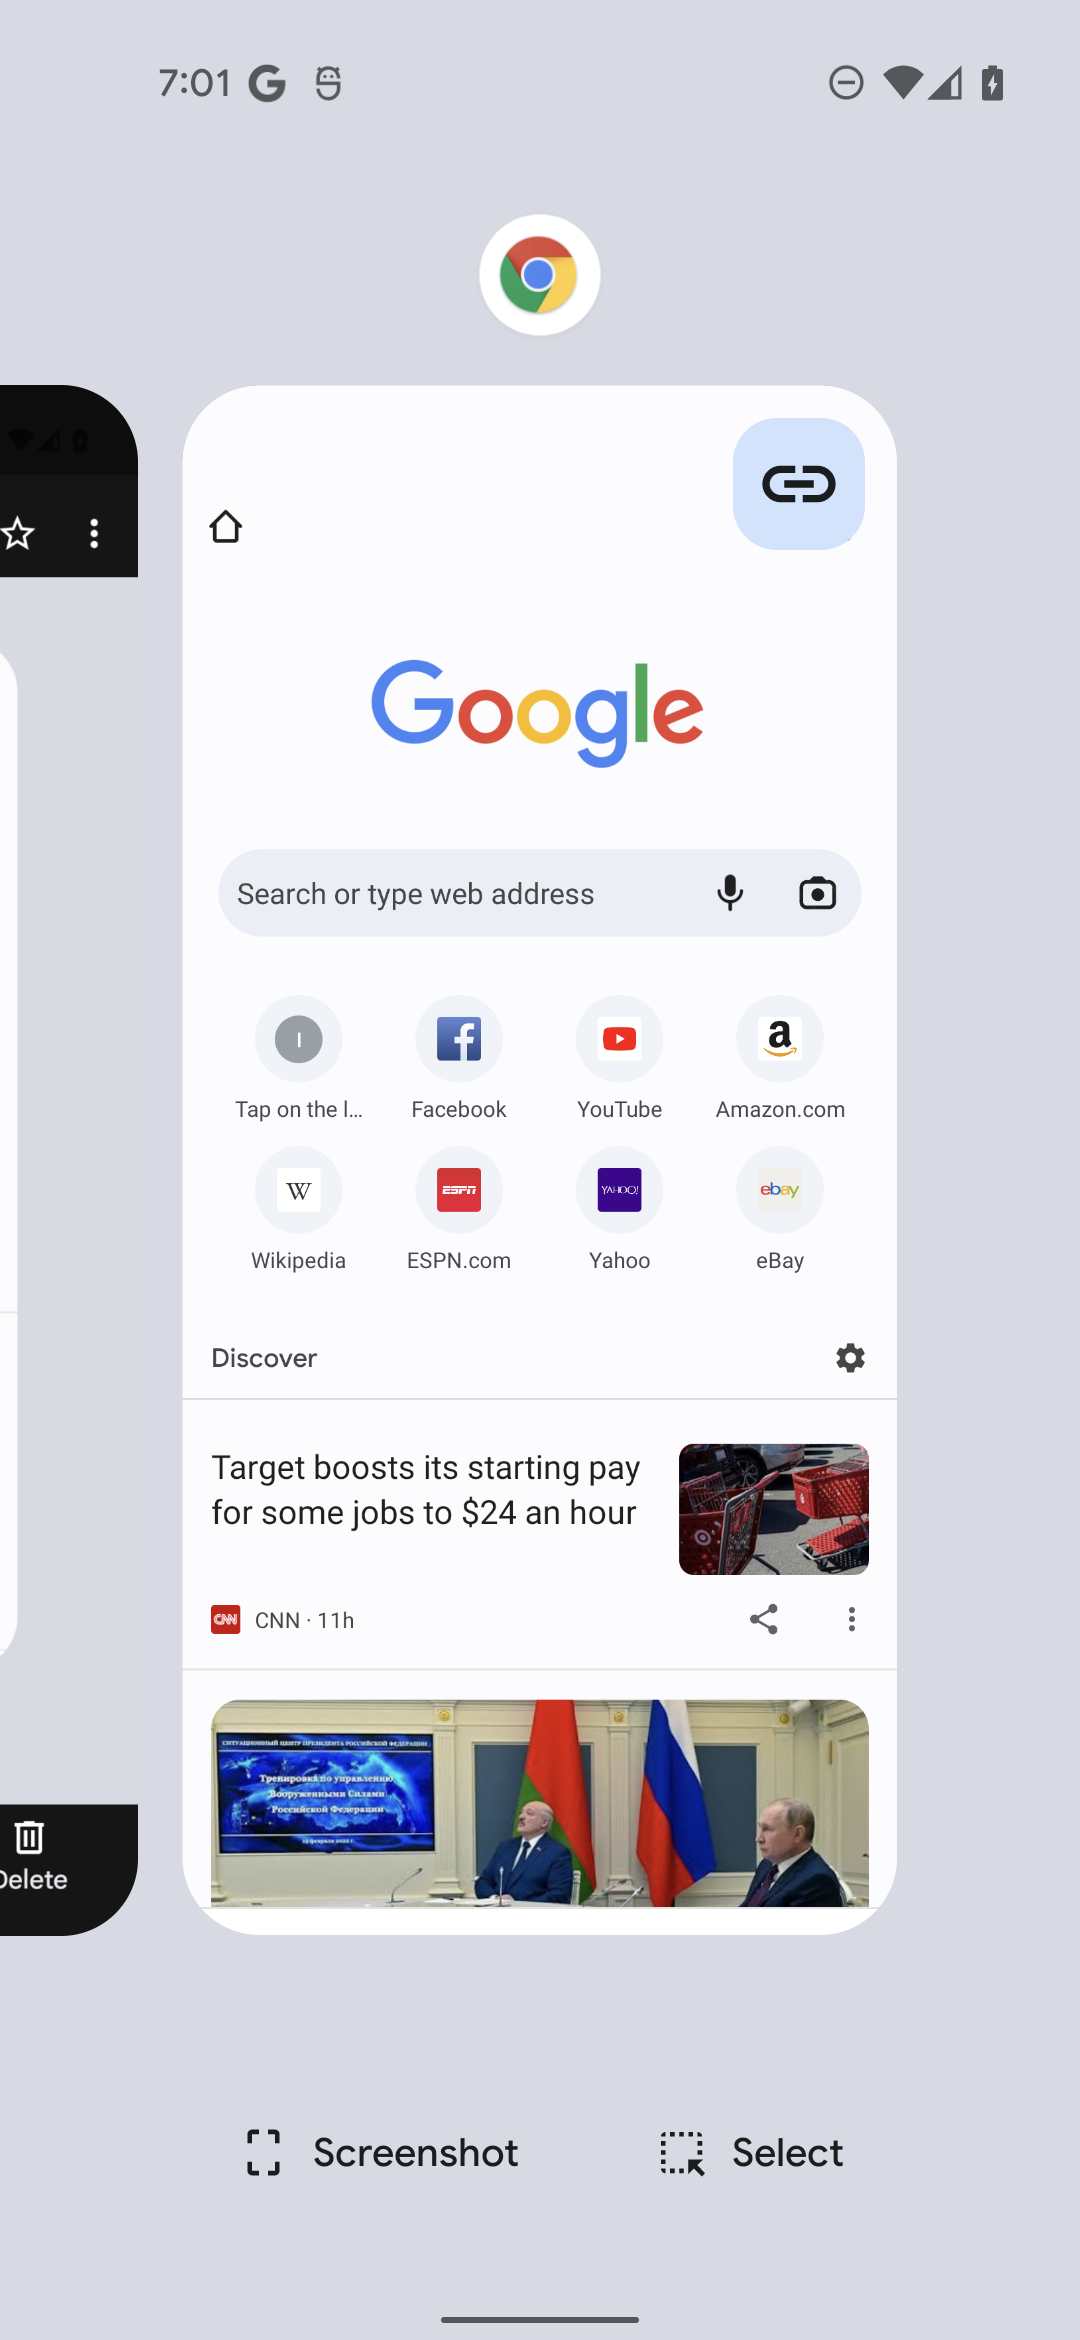
\includegraphics[width=0.3\columnwidth]{fig/recents-screen.pdf}
\caption[Recent Apps Screen Example]{A screenshot of Recents screen showing that Chrome is recently accessed. However, a spyware app will not appear in the recent screen (if it chooses to hide from the recent screen), despite that one of its Activities is recently created and displayed.}
\label{fig:recents_screen}
\end{figure}


\subsubsection{Mitigations}
For apps that seek to hide their icons, our recommendation is that Android should enforce stricter requirements on what apps can hide icons (e.g., the three requirements from Android 10 build r1 to r14 mentioned in footnote~\ref{footnote:hide_icon}).
Most apps that run on Android phones should be required to have an icon. In the case of exploiting TV app features, while we
understand that running apps with only \texttt{LEANBACK\_LAUNCHER} activities on
Android phones increases compatibility, such a feature leads to abuse as Spy24
has already demonstrated.

Launching apps by predetermined signal from another app is not only used for
malicious purposes but also for benign purposes (e.g., dial pad can be used for
testing and numerous benign apps use a browser link to open themselves).
While browser links can be easily tracked by examining the manifest, currently
users have no way to discover if apps can launch themselves with hidden codes.
The difficulty is in part because hidden codes are used dynamically during
runtime: the outgoing dialed number is sent to apps, and apps can freely decide
what actions to perform based on the number received. This design makes it hard
for the Android system to identify what hidden numbers are being tracked by each
app.  One possible mitigation is to allow users to review apps that can receive predetermined signals (e.g., a list of apps that listen for the
\texttt{NEW\_OUTGOING\_CALL} intent or have intent filters for specific browser links,
perhaps as part of the privacy dashboard).

One potential fix to stop apps from hiding from the Recents screen is to enforce
having at least one activity per app in the Recents screen.




\subsection{Persistence}
\label{subsec:persistence}
This section describes the methods used by spyware apps to persist on the target
device by obscuring the uninstallation process and creating ``diehard'' services
(automatically restarting themselves after stops and reboots).

%\subsubsection{Capabilities}

\subsubsection*{Capability \#7: Obscuring the Uninstallation Process}
\begin{figure}[t]
\centering
\includegraphics[width=0.6\columnwidth]{fig/DA_pdf.pdf}
\caption[Disabling Uninstall Buttons Example]{An example of an app disabling both the
Force Stop and Uninstall buttons on Android 6.}
\label{fig:da}
\end{figure}
One way to prevent users from stopping and uninstalling an app is by
disabling the Force Stop and Uninstall buttons (see
Figure~\ref{fig:da}).  For Android versions below 7.1,
these buttons can be disabled simply by registering the app with
\texttt{Device Administrator} (DA) privileges (as detailed in prior
work~\cite{shan2019device}). To enable these two buttons, the user
would have to deactivate the device administrator privileges for the
app.
%
Since Android 7.1, while the Force Stop button is disabled for DA
apps, the Uninstall button will remain enabled even if the app
registers as DA.  As a result, users can uninstall DA apps
directly~\cite{shan2019device}. Overall, I observe 11 apps that
register as DA.
%% \damon{this is really cryptic and difficult to
%% understand.}\alex{fixed}

Two apps, Cerberus and Mobile-tracker-free, directly interfere with the
uninstallation process, a behavior often observed in Android
malware~\cite{shan2019device,aljarrah2016maintaining}. Cerberus employs a series
of mechanisms to stop users from deactivating it as a DA app or
uninstalling it. These include trying to lock the device by invoking the
\texttt{lockNow} method of the \texttt{DevicePolicyManager} class and starting
an activity that blocks users from clicking on any buttons. Mobile-tracker-free,
on the other hand, tries to stop users from uninstalling it by starting an
Activity that blocks the uninstallation screen and requests a password set
by the abuser to proceed.

\subsubsection*{Capability \#8: Creating Diehard Services}
%\alex{a new title?}
%
Spyware apps strive to always be executing on the target device so
that they can collect as much information as possible.  I focus on
the ``diehard'' mechanisms that apps use to automatically restart
themselves after being stopped by the Android system (e.g., due to low memory) or after device
reboots. Echoing the diehard implementations discovered in prior
work~\cite{shao2019lightweight,zhou2020demystifying}, I observe two
main ways used by spyware apps to create diehard services. I also note
a third approach that appears to originate from the spyware ecosystem
and be a byproduct of other capabilities.

\textbf{Leveraging Scheduling Frameworks.} Scheduling frameworks such as Android's
\texttt{JobScheduler}~\cite{JobSched94:online} and
\texttt{AlarmManager}~\cite{AlarmMan39:online} enable apps to repeatedly
restart. Apps can schedule to be restarted either when they are
first started or when they are being terminated by the system. To schedule
themselves to be restarted shortly after they are terminated, they override the
\texttt{onDestory} function, which is called before the app is terminated by the
system.

\textbf{Monitoring System Broadcasts.} Monitoring system broadcasts offers another way to wake up apps if they are not running already. Android sends broadcasts when various system events occur~\cite{Broadcas25:online}, and apps that monitor these system broadcasts will be woken up if they are not running already. Table~\ref{tab:monitor_broadcast} lists various systems broadcasts and the number of apps that monitor them.\footnote{Only a small number system broadcasts can be used to wake up apps after the restrictions introduced in Android 8~\cite{Implicit72:online}. I only consider these system broadcasts.} The spyware apps in our study predominantly use the \texttt{BOOT\_COMPLETED} broadcast. Monitoring
\texttt{BOOT\_COMPLETED} allows spyware apps to restart themselves
after the device reboots: the Android system will send a
\texttt{BOOT\_COMPLETED} system broadcast upon reboot, and spyware apps that listen
for this broadcast will automatically restart themselves. While \texttt{NEW\_OUTGOING\_CALL} and \texttt{SMS\_RECEIVED} are also popular, I note that they serve dual purposes (\texttt{NEW\_OUTGOING\_CALL} can be used to launch a hidden app and \texttt{SMS\_RECEIVED} can be used to monitor SMS messages).

\textbf{Listening for Accessibility or Notification Events.} Apps that choose to register as an
\texttt{AccessibilityService} or
\texttt{NotificationListener- Service}
can also survive device
reboots. However, unlike the two techniques described above,
\texttt{AccessibilityService}
is less reliable because it can be
turned off by Android for battery saving reasons~\cite{AndroidA0:online,Accessib46:online}.


\begin{table}[t]
  \centering
  \begin{tabular}{lr}
    System Broadcast         &\# of Apps  \\
    \midrule
    BOOT\_COMPLETED          &10          \\
    SMS\_RECEIVED            &9           \\
    NEW\_OUTGOING\_CALL      &9           \\
    PHONE\_STATE             &6           \\
    ACL\_DISCONNECTED        &1           \\
    ACL\_CONNECTED           &1           \\
    LOCKED\_BOOT\_COMPLETED  &1           \\
    WAP\_PUSH\_RECEIVED      &1           \\
  \end{tabular}
  \caption{System broadcasts and the number of apps monitoring them.\label{tab:monitor_broadcast}}
%  \vspace*{-1cm}
\end{table}

\begin{facingcaption}{table}
\caption[Systematization of Commodity Spyware Vulnerabilities]{Systematization of commodity spyware vulnerabilities. Circles denote the severity level of the insecurity. \protect \partrating\ indicates at least one instance of the insecurity; \protect \rating{100} indicates all app functionality is insecure; * indicates URLs are temporary and expire.
          Shading added to improve readability.}
\label{tab:apps_spyware_vuln}
\renewcommand\tabularxcolumn[1]{>{\RaggedLeft\arraybackslash}p{#1}}
\parindent=0pt
\setbox0=\vbox{%
\vsize\textwidth
\hsize\textheight
\linewidth\hsize
\columnwidth\hsize
\textwidth\hsize
\textheight\vsize

\begin{tabular}{lm{2.5cm}m{2.5cm}m{4.2cm}m{2.9cm}m{3.0cm}}
%		\toprule
		Spyware Apps & Eavesdropping Sensitive PII & Cross-account Request Forgery & Unauthenticated Access to Victim Data & Poor Data Retention Practices & Unauthenticated SMS Commands \\
		\midrule
		mSPY & \partrating &  & Images &  &\\
		Mobile-tracker-free & & & Streaming & & \rating{100}\\
		Clevguard & \partrating & & Images* & &\\
\ltgrey 	HoverWatch & & & Audio* & &\\
\ltgrey 	Flexispy & \rating{100} & & Images/Audio* & &\\
\ltgrey		Spyic &  &  & Images* & \partrating &\\
		Spyhuman & & & Images/Audio & &\\
		TheTruthSpy & \rating{100} & \rating{100} & Images/Audio & \rating{100} &\\
		iKeyMonitor & & & & &\\
\ltgrey		Cerberus & & & Audio &  & \\
\ltgrey		Spy24 & & & Streaming* & &\\
\ltgrey		Spapp & & & Images/Audio/Streaming & \partrating & \rating{100}\\
		Meuspy & & & Images/Audio & \partrating &\\
		Highstermobile & & & Images &  &\\
%\ltgrey		LetMeSpy & & & & &\\
%		Spylive360 & & & Images/Audio & \rating{40} &\\
%		Talklog & & & & &\\
%		\bottomrule
	\end{tabular}


\singlespacing
}
\centerline{\rotatebox{90}{\box0}}
\end{facingcaption}


%% \geoff{so ``waking
%% up apps'' is just for surviving reboots?  I might want to rename}\alex{fixed.
%% techinically apps can be woken up in many ways...after being stopped. by
%% \texttt{BOOT\_COMPLETED} seems to solely used for waking up purposes}

%We also note that the old \texttt{camera} framework has an API called
%\texttt{getSupportedPreviewSizes}, which supplies a list of supported preview
%sizes\alex{not sure about camera2 framework}.

%While the API document s

\subsubsection{Mitigations}
Apps that seek to persist by registering as device administrator will
no longer be successful as users can uninstall them on most devices
running Android 7.1 or above. For apps that seek to interfere with the
uninstallation process by creating activities or locking the device,
past literature on malware defense~\cite{fernandes2016android,
  aljarrah2016maintaining} has suggested improving attack detection
and introducing system level support for detecting and reacting when
an app window is covered.
% \geoff{are there suggestions from the malware papers?}\alex{fixed}


Prior work~\cite{zhou2020demystifying} has investigated various ways
of creating diehard apps. According to the authors, the diehard
mechanisms I observe are very resilient and can only be effectively
stopped via a force stop.
%% \geoff{``the above abuses can only be effectively stopped'' --- by abuse do you
%% mean spyware activities in general, or just the methods for keeping apps
%% alive/waking up apps?}\alex{fixed}
%% However, it is unlikely that users would force stop instead of
%% uninstall a suspicious app after they have discovered it.
Additionally, the fact that many spyware apps register as device administrator
creates another layer of complication --- while apps registered as DA may be
uninstalled directly after Android 7.1, the force stop option is disabled,
making it difficult for users to stop the spyware apps (unless they uninstall
it).
However, even if apps prevent a force stop, users can still uninstall
them.
I also recommend adding a dashboard for monitoring apps that will automatically
start themselves.\footnote{We note that some Android phones (e.g., Xiaomi) have a
built-in dashboard for managing apps that can automatically start
themselves~\cite{HowtoDis42:online}.}

%\geoff{so...no mitigation then?}\alex{fixed}


% \subsection{Discussion}
% TBD


% Before diving into the actual implementation, I first detail the general
% process of building customized camera implementations. Each camera is in
% Android is a \texttt{CameraDevice} and is responsible for producing raw data
% frames~\cite{Cameraca74:online}. Apps receive these raw data frames by
% specifying an output  buffer, which for example could be a
% \texttt{SurfaceView}, \texttt{ImageReader}, \texttt{RenderScript.Allocation},
% or \texttt{TextureView}~\cite{Cameraca74:online}.

% In practice, I observed X different customized camera implementations: (1)
% through creating 1x1 pixel SurfaceView.

% To create a camera session, provide it with one or more output target buffers
% your app can write output frames to.

% The first implementation creates 1x1 pixel previews. It requires the
% \texttt{SYSTEM\_ALERT\_WINDOW} permission to draw over other apps.
% Applications


\section{Spyware User Data Protection}
\label{sec:data-leak}

%\damon{at a high level I need to make it clear that I only attempted to access our own data and I should also include citations to prior news articles and industry reports that overlap with our findings.}

%% \geoff{need to describe the various infrastructure elements involved
%%   (device, accounts, servers) and lifecycle steps (when does the
%%   abuser create/setup/access an account, does the abuser download and
%%   install the spyware on the victim's device after creating an
%%   account, abuser account registration vs victim device registration
%%   to an abuser's account, high-level of how the abuser remotely
%%   controls the spyware on the victim's device).  might also go earlier
%%   in the paper for context on app implementation, but particularly
%%   needed for understanding the data protection part.}
%\sumanth{Not sure where this should go. Here in the intro?} \geoff{yes put it here for now, don't
%  worry about the flow with other parts for now}

In this section I assess how well spyware apps secure the user data they exfiltrate and store.
For this assessment, in addition to the victim and the abuser, we
consider a third actor: an external attacker who seeks to undermine the
security of the spyware app.  The attacker's goal is to exploit any
integrity, authorization, and authentication issues with the spyware
app to access victim data as a third party.
% that the attacker is not supposed to have access to.

%% When discussing each of the security issues below, I note further
%% assumptions about the attacker that are specific to a particular
%% issue.

%% Table~\ref{tab:apps_spyware_vuln} summarizes the threats we
%% investigated and shows which apps are susceptible to them.

We start by describing our
methodology for investigating the data protection practices of the
spyware apps, and then discuss each of the vulnerabilities I uncovered (summarized in Table~\ref{tab:apps_spyware_vuln}).

\subsection{Methodology}
\label{subsec:experiemental_setup}

%\sumanth{Revised methodology section 4.1}
For each app I analyzed, I obtained an account (providing payment
information when necessary) and registered the app on a Pixel 2 XL
Android phone running Android 10.
%% I used man-in-the-middle (MITM) traffic inspection to perform our
%% network analysis on each spyware app.

To identify apps sending data from the device to the backend servers via unencrypted connections I used \texttt{tcpdump},
listening on a Windows 10 machine interface configured as a mobile
hotspot, to capture and inspect app traffic over the network.  We
configured the Android phone to connect to the PC and recorded all
traffic exchanged with the app servers, without any proxy in between
(avoiding any potential TLS handshake failures due to certificate
pinning).

To study the interactions between the spyware web portal interface and
the spyware backend servers, I used the open-source \texttt{MITMProxy} tool to
decrypt HTTPS traffic.  This configuration gave us access to
authentication tokens (session cookies, secrets, etc.) for conducting
forgery attacks on our test accounts.  I were able to login to all
portals without error (e.g., there were no issues with certificate
pinning).  I also analyzed the HTML content displayed via the spyware
web portal interface, extracting the URLs linked to uploaded user
media (images, audio, etc.).  I then performed a sequence of
experiments that tested and verified each insecurity listed in
Table~\ref{tab:apps_spyware_vuln}.

% I installed a trusted PEM certificate (generated
% by the proxy) on the phone, adding the certificate to the list of user
% store certificate authorities.

%% \geoff{could also aggregate the specific methodology parts from the
%%   subsections here}

%% For each app I analyzed, I obtained an account (providing payment information when necessary) and registered the app on a Pixel 2 XL Android phone running Android 10. I used a man-in-the-middle (MITM) traffic inspection approach to perform our network analysis on each spyware app, focusing on outgoing requests from each app that I manually installed on the Android phone. I leveraged the open-source MITMProxy tool to inspect outgoing requests, which I setup and ran on a Windows 10 PC noting its IP address. I then configured the Android phone to connect to a mobile hotspot setup on the PC, and configured a manual proxy to route all traffic to port 8080 - that the traffic inspector actively ran on. In order to decrypt TLS traffic, I installed a trusted PEM certificate (generated by the traffic inspector) on the phone, which adds the certificate to the list of user store certificate authorities. For each spyware app, I installed the mobile app onto the Android phone, logged in using the abusers credentials and ran through the sequence of experiments which test each insecurity listed in table \ref{tab:apps_spyware_vuln}.
%% I also analyzed the spyware web portal interface and extracted the path for uploaded user media (images, audio, etc) which I used for the following experiments.

\subsection{Results}

Table~\ref{tab:apps_spyware_vuln} summarizes the threats we
investigated and shows which apps are susceptible to them.
%
We describe each of the threats in turn, summarizing its context, its
associated threat model, any additional methods I employed, and the
specific results I discovered for the vulnerable apps.

%% I start by briefly describing each insecurity, along with the threat
%% model and experimental setup used to identify the insecurity. I then
%% discuss a subset of the apps which demonstrate each insecurity. To
%% structure our analysis, I focused on security mechanisms for
%% protecting sensitive user data.

%We are less interested in flows that do not aid in compromising the app or user data; for example, apps that are using unsecured HTTP connections for non-sensitive functionality.

%% \geoff{the structure of these subsections results in some redundancy
%%   across the various parts, which is not ideal.  but it does have the
%%   virtue of being explicit about each of the parts.}

%\subsubsection*{Insecurity \#1: Submitting sensitive victim or abuser PII over the network}
\subsubsection*{Insecurity \#1: Eavesdropping Sensitive Personally Identifiable Information (PII)}
%\subsubsection{Eavesdropping sensitive PII}

Some spyware apps transmit highly sensitive victim data, such as photos,
texts, and location, from the victim device to the spyware backend
servers using unencrypted HTTP connections.  A MITM attacker who
eavesdrops on the same communication channel (e.g., same WiFi network)
could collect all data and credentials sent unencrypted
over the network.  Furthermore, credentials leaked over the network enable
an attacker to login to the abuser's account and gain access to all of
the victim's data exfiltrated by the spyware.

\textbf{Threat Model.} I assume that the attacker can eavesdrop on
all messages sent by the mobile device infected with spyware (e.g.,
the attacker uses the same WiFi network as the victim, and the WiFi
network is not using link-layer encryption).

%% I also assume that the network used when eavesdropping is unencrypted
%% (e.g., a WiFi network not using link-layer encryption).

%% \geoff{doesn't the WiFi network need to
%%   be unencrypted (not use link-layer encryption)?} \sumanth{Addressed}

\textbf{Experimental Setup.}
%% To uncover sensitive data flows, I utilized the spyware's
%% functionality and observed the outgoing network traffic from the
%% target device.
We filtered the captured traffic to observe network activity from each app over
insecure channels like HTTP, and used a combination of search and
manual inspection to analyze the recorded traffic for sensitive data
such as leaked credentials (user names, email addresses, passwords),
text messages,
% call logs,
etc.

%% Filter's were setup to flag any network activity over insecure
%% channels like HTTP. These packets were manually analyzed to see if
%% they leaked passwords, messages, call logs, etc. Similarly I flagged
%% packets containing sensitive PII's (i.e., user/abuser email) using
%% regex matching.

%% \damon{did I check for password, sms, call logs, messages?}
%% \sumanth{Added a line above that I analyzed insecure packets to see
%%   if they leaked all these.}

\textbf{Results.}  Four spyware apps in our study leak at least some
of their data using vulnerable communication channels.  TheTruthSpy
submits all of its data over HTTP, and it leaks the abuser's
credentials for TheTruthSpy servers (abuser email address and
password) in the authentication request during app setup.
%% It also leaks the abuser email address
%% in response to an unauthenticated request for registration information.
%% TheTruthSpy also leaks the abuser's email address in the response to
%% an endpoint called during setup time.
%% \geoff{victim's?}
%% \sumanth{Edited to make it clearer. There are 2 cases - email and pwd
%%   leaked in a request during setup time, and just the email leaked in
%%   the response every time a particular endpoint is called}.
%% \geoff{``endpoint'' is still a bit vague? if the email address leak is
%%   also during setup, then I think I can leave it out (the full
%%   credential leak is already a worse case)}
mSPY leaks only
the upload path for its images in an HTTP response back to the
victim's device when the image upload succeeds.
%\sumanth{Added this for Clevguard}
Clevguard uploads its images over HTTP, making it is possible for an attacker to reconstruct the image from the payload.  Flexispy uses
HTTP for all of its communication, but it implements a custom
encryption protocol for the data it sends.  However, a previously
discovered flaw in Flexispy's encryption makes it possible to
intercept personal data sent over the
network~\cite{Stalking85:online}.

%% I observed 3 spyware apps send their data - like texts, images,
%% locations - over plain HTTP protocol. \textbf{TheTruthSpy} submits all
%% its data over HTTP. Further, it leaks both the abuser email and
%% password during app setup time (when authenticating), and the abuser's
%% email during setup time. \textbf{mSpy} on the other hand leaks only
%% the upload path for its images in a HTTP response back to the victim's
%% device once the upload is successful. While both these apps send data
%% in the clear, \textbf{Flexispy} implements a custom encryption
%% protocol even though it sends data over HTTP. However, a perviously
%% discovered flaw in Flexispy's encryption makes it possible to
%% intercept personal data being sent over the network
%% \cite{Stalking85:online}.

\subsubsection*{Insecurity \#2: Cross-account Request Forgery}
%\subsubsection{Cross-account request forgery}

Knowing a particular user identifier, or a file path that provides access to images, audio, or video on the server, an attacker can use valid
cookies from one spyware account to access data or perform actions in
the accounts of other spyware users.

\textbf{Threat Model.} The attacker can register a spyware account and
log into it. Using a MITM traffic inspector (similar to our proxy
described in Section~\ref{subsec:experiemental_setup}), an attacker
can intercept and replay authenticated requests from their account. We
assume the attacker knows the ID of the targeted user's account ---
either through enumeration, or from the ID being leaked over the
network or in a public data dump~\cite{mSpybrea38:online,
  Companyt8:online, HackerSt66:online, Cerberus12:online,
  Stalkerw59:online}.

%% \damon{this is cryptic, I would suggest directly stating that the
%%   attacker can register/purchase a spyware account and log into it.}
%% \geoff{still cryptic :-) \sumanth{Reworked this section. Hope its
%%     better now :)}}

\textbf{Experimental Setup.} I used two accounts for each app, one
for the attacker and the other as the targeted spyware user.  I then
recorded and replayed authenticated requests from the attacker's
account to the targeted user's account, substituting the ID of the
targeted user's account in the requests without changing authorization
tokens provided by the attacker's account (e.g., session IDs, API
keys).  I only replayed requests to our test accounts, and
made no attempt to access content belonging to any other account.

%% \sumanth{Reworked based on Damon's feedback}\damon{this need to be
%%   improved to better describe that I had two accounts and that we
%%   checked for cross-account data leakage. I should also be clear that
%%   I only probed our own accounts and I did not attempt to access any
%%   content that potentially belonged to another person's account.}

\textbf{Results.}  Only one of the apps in our study is vulnerable to
cross-account request forgery.
%% I disregarded apps which have API
%% structures with no IDs that identify users or devices, and instead
%% rely solely on session IDs for authentication and
%% identification.
%% \sumanth{Added this to tie well with results in table}
%% \geoff{I'm still not sure the distinction between ``No'' and ``--'' in
%%   the table.  does ``--'' mean that by design the app is not
%%   suscectiple to CARF?  and No means that the app's design could be
%%   susceptiple but its implementation is correct?} \sumanth{Yes, exactly!}
With TheTruthSpy, it was possible to
access all data (messages, contacts, locations, images, etc.)  in the
targeted account using a cookie provided by the attacker's account,
and simply swapping the attacker's device ID with the targeted
account's device ID in requests to TheTruthSpy server.  Furthermore,
when I registered multiple test accounts in succession, I noticed
that the device ID that TheTruthSpy assigns to a new device is a six-digit
integer which increases incrementally when new devices are registered.
%% \damon{how did I determine that it increased
%%   incrementally?}\sumanth{I see newer accounts always get assigned
%%   higher numbers which are very close by to older ones. I tested with
%%   2 accounts and found the deviceIDs were close by.}
The combination of insecure access controls across accounts and
predictable device IDs makes it possible for an attacker to retrieve
data from other accounts without needing to identify the device ID
beforehand.

%% by swapping the
%% device ID of a target account, while using valid cookies provided by
%% the first account. Furthermore, the device ID TheTruthSpy assigns to a
%% new device is a 6 digit integer which increases incrementally when new
%% devices are registered. \damon{how did I determine that it increased
%%   incrementally?}\sumanth{I see newer accounts always get assigned
%%   higher numbers which are very close by to older ones. I tested with
%%   2 accounts and found the deviceIDs were close by.} The combination
%% of insecure access controls across accounts and predictable device ID
%% makes it possible for an attacker to retrieve data from other accounts
%% without needed to know the device ID beforehand.

% \sumanth{TODO: Any other CARF in other apps?}

%\subsubsection*{Insecurity \#3: Leaking sensitive data on public server URIs}
\subsubsection*{Insecurity \#3: Unauthenticated Access to Victim Data}
%\subsubsection{Unauthenticated access to victim data}
\label{sec:leaky-urls}

%% \geoff{would be good to describe the scenario: some apps use CDNs or
%%   backend servers to store media data (do I know why? cost?), and the
%%   URLs they generate to the media data are unauthenticated.  the idea
%%   is to note the distinction between URLs to content on the app's server
%%   vs URLs to media stored on different infrastructure (which is my
%%   understanding of what's going on here, which may be wrong?)  either
%%   way, I want to give some sense/intuition for why URLs for accessing
%%   this content is different than other content stored on the spyware
%%   servers.} \sumanth{Good point! I've added this in the intro of the section below. One thing missing might be the reasoning as to why they choose to store media on different servers. Cost might be the main reason yes.)} \geoff{thanks, edited}

Many of the spyware apps use different backend infrastructure to store
and deliver media data that is distinct from the servers that
abusers use to access the app dashboard (e.g., abusers login
to the dashboard via the website domain in Table~\ref{tab:apps_selected}, but
the app may use a CDN to deliver images and videos).
This separate infrastructure
includes cloud storage (e.g., AWS S3 buckets), content distribution
networks, and other shared hosting services, all of which are
presumably cheaper to use for serving media data.
% I observed that
Some of the spyware apps are less careful about protecting the
data that they store on this hosting infrastructure, often allowing
unauthenticated access to the URLs they generate to stored media data.
Further, I observed user data stored in predictable URLs that make it
possible to access data across different accounts, protected solely
through security by obscurity and vulnerable to enumeration. Table~\ref{tab:apps_spyware_vuln} lists
the kinds of data leaked in public URLs for the apps studied. Failure
to authenticate access to user media (images, audio, etc.) using
mechanisms like cookies is a common example of this category of
vulnerability.

\textbf{Threat Model.} I assume that the attacker has knowledge of
the media upload path for the app based on studying media paths
revealed using accounts owned by the attacker.  For apps that use the
device ID in URL path components, I also assume the attacker knows
the targeted device ID.

\textbf{Experimental Setup.} To discover sensitive data leakage, we
focused primarily on URLs used to store media artifacts (images,
audio, video, etc.).  I extracted these URLs by examining the
browser-generated HTML content when accessing the dashboard in the
spyware account.  I only attempted to access media upload paths from
our test accounts, and made no attempt to access content belonging to
any other account.

%% \geoff{how did you collect URIs using the attacker's account?}
%% \sumanth{Addressed. Also added another statement to make sure I are
%%   clear that I collected media links from our own accounts}

\textbf{Results.}  Six of the apps in our study store their data in
public URLs accessible without authenticated access.  I disregarded
apps which store data in URLs that, although public, expire after a
short duration (e.g., Spyic's links to images expire after 1,800
seconds).

% I also disregard those apps which required authenticated
%(cookie-based) access to data. \geoff{not sure the distinction between
%  this case and other authenticated account access?}

Highstermobile stores its images with a URL scheme as a concatenation
of the image upload timestamp (UNIX timestamp with seconds precision)
and a double digit random number, with no other per-device ID in the
path (e.g.,
\texttt{\url{https://domain.com/path/photo_<timestamp><00-99>.png}}).
% \sumanth{\url{https://evt17.com/iphone/uploads/gallery/image/thumb/photo_<UNIXTimestamp><00-99>.png}}.
Since an attacker could plausibly iterate over a short range of
timestamps and random digits, this naming scheme makes it
straightforward for an attacker to gain unauthorized access to media
stored on the server for other accounts.

Cerberus and Spyhuman use public URLs that are a combination of device
ID and Unix timestamp
% (also Unix timestamp with seconds precision)
(e.g., \texttt{\url{https://domain.com/<DeviceID>-<timestamp>.ext}}).
While both of them require the attacker to know the device ID before
hand, an attacker could for instance obtain the device ID from data
dumps made public in breach attacks~\cite{mSpybrea38:online,
  Companyt8:online, HackerSt66:online, Cerberus12:online,
  Stalkerw59:online} or with physical access to the device.
%% \geoff{I added this, are there better scenarios?} \sumanth{Maybe also
%%   from public data dumps which have device metadata?}
Cerberus stores audio insecurely using the device IMEI as the device
ID.  Spyhuman stores both its images and audio insecurely using the
Android serial number as its device ID.  With both apps, an attacker
knowing the device ID could plausibly iterate over a short range of
timestamps to retrieve data stored on the server.

% \url{https://www.cerberusapp.com/audio/<DeviceID>-<UNIXTimestamp>.mp4}
% \url{https://dwnlnew.webdown2.com/rec/<DeviceID>/<UNIXTimestamp>/file.mp3}

Three other apps store data on servers using public URLs that rely on
security through obscurity, but they generate URLs that are neither
enumerable or predictable.  For instance, Spy24 allows WebRTC remote
streaming through a public URL based on a request ID generated by the
app, Spapp requires two alphanumeric keys to access image and audio
files on the server, and Meuspy generates unguessable URLs to
store images and audio.  Although certainly not good security
practice, the risk associated with unauthenticated access is lower
than for the other apps I discussed.

%% these three apps do not implement
%% good security practice by solely depending on security by obscurity,

%% \geoff{conclusion?  not good security
%%   practice but lower risk than the other apps?} \sumanth{Added.}

% complicated

%% Among the other 3 apps which leaked data on public server, all of them generate URIs which although public, is neither enumerable or predictable. These rely solely on Security through obscurity. \sumanth{e.g \textbf{Spy24.app} (which allows WebRTC remote streaming through a public URL based on a request ID generated by the app), \textbf{Spapp} (which requires 2 alphanumeric keys to access any image/audio on the server) and \textbf{Spylive360} (which generates complicated URLs to store images/audio)}

\subsubsection*{Insecurity \#4: Poor Data Retention Practices}
%\subsubsection{Poor data retention practices}

%% \sumanth{I rewrote this section to better explain what I had in mind.}

Some spyware apps have poor data retention practices that prevent
victim data from being deleted from the spyware servers. These data retention issues pose serious security and privacy risks~\cite{santhanam2022scraping}. A data breach could expose residual victim PII which has persisted even if, for instance, the abuser has deleted their account.

%% , in some cases because the data is either unaccessible by the abuser
%% or unassociated with any account.



%% All there of these cases involve unauthorized transmission of data which remains on the server indefinitely, and is either unaccessible by the abuser or unassociated with any account. These scenarios poses a risk if a data-breach exposes residual victim/attacker PII which has continued to persist.

%% \geoff{if I just have one app that has all of these risks, then we'll
%%   want to rework the story a bit}

%% Again, all data uploaded in both of these cases has the potential to
%% be leaked in a data breach.

%% \sumanth{I rewrote this section to better explain what I had in mind. Broadly speaking there are 3 cases here - Unassociated data sent without logging in, data sent but inaccessible without purchase, data sent after license expires or app is deleted. I've moved the part of 'delete' not actually deleting data to the end of section 4 along with the other misc stuff.}

%\geoff{who installed the app but never
%  used it?  an abuser who decided not to use it?  is this a compelling
%  risk?}

%% \geoff{do the apps provide the capability for the abuser to delete
%%   uploaded victim data via their server account?  if so, did I test
%%   to see if that data is actually deleted?  if not, there might not be
%%   time to do it for the submission, but is something to add for later} \sumanth{Yes, for apps which allowed the delete account option, I tried to see if both uploaded media and replaying endpoints to get, and have results for this}

%% Some apps send user data (like text messages, images, keylogger activity) to the spyware app servers before the abuser logs in/sets up the account. In some cases, this data is never visible to the attacker but is stored on the server. In some cases, user data (like images, audios, text messages, etc) persists even after explicitly deleting the account associated with the abuser. Further, in the event the license expires some spyware apps continue to send data to the backend servers, unaware of the expired license. This poses a particular issue if a data-breach exposes sensitive user data of victim's, who might have installed but never used the app \cite{esetandr4:online}

\textbf{Threat Model.} Data uploaded to the spyware servers and never deleted poses a long-term risk to being made public in data dumps associated with breach attacks.
%\sumanth{I'm not sure if this has a threat model because this doesn't have an attacker per say.}
% \geoff{data never deleted poses long-term risk to data breaches?} \sumanth{Added.}

\textbf{Experimental Setup.}  To discover poor data retention practices, I analyzed network traffic generated after the app license expired, but with the victim device still logged in.  I also tested
access to media on deleted accounts using their public URLs up to
seven days after deletion of the account.
%\sumanth{Added this line.}

%% Network traffic from the target device was captured and analyzed
%% before the abuser logged in and after the license expired.  Data
%% uploaded to the server was tested for persistence after the account
%% was expired.

\textbf{Results.}  Four of the apps in our study demonstrate poor data retention practices.

Consistent with its other data vulnerabilities,
TheTruthSpy also has data retention issues.
% \sumanth{Based off of reviewer C's comments, I omitted the data sent before registration result here. I now only talk about the data sent after license expiry and data retained after account deletion.}
It continues to send
data from the victim's phone (e.g., text messages, images, keylogger
activity) to its servers after the app license expires. Further, it persists some data after the abuser
deletes their spyware portal account and the data associated with it.
%
%before the abuser even sets up their account.
%The exfiltrated data is never associated with an account and thus
%cannot be deleted even after logging in to the spyware portal.
%
%% \geoff{how is the exfiltrated data associated with the account if it
%%   is sent before the account is set up?} \sumanth{Clarified}
%% \geoff{who installed the app but never used it?  an abuser who decided
%%   not to use it?  is this a compelling risk?}
%It also continues to exfiltrate data to its servers after the app license expires.
In particular, images uploaded from the victim device persist after
account deletion, and the images remained accessible through the
public URLs used to access them (Section~\ref{sec:leaky-urls}).

%% abuser does not uninstall the logged-in app \sumanth{This seems like a
%%   common scenario abusers might do} \geoff{it does.  have we
%%   systematically tested what happens across the apps when I delete
%%   the portal account but leave the app on the device?} \sumanth{TLDR - I did capture traffic for this scenario, but the results are fuzzy, so I can omit this.}

%% Similarly, the exfiltrated data continues to be uploaded even after the abuser deletes their account, but does not uninstall the logged-in app \sumanth{This seems like a common scenario abusers  might do} or even in case the app license expires. The uploaded data, even though valid, is no longer accessible by the abuser.

Spyic has a data retention issue resulting from its trial usage
model.  When installed for trial use, Spyic uploads data from the
victim device to the server.  But it only allows access to its portal
after the abuser has purchased a subscription.  If the abuser decides
not to purchase the spyware, victim data persists indefinitely on
Spyic's servers (presumably in anticipation of the spyware user
eventually deciding to pay for a license).

%% \geoff{I added this statement, is it accurate?  do I think that
%%   Spyzie will retain the data indefinitely in anticipation of someone
%%   eventually paying?}
%% \sumanth{Yes, afaik there's no option to delete
%%   data on Spyzie.io. https://spyzie.io/privacy.html says you can go do
%%   so after loggin in (but there's no option on the portal to do this)
%%   or contact them to delete your data}

%\sumanth{TODO: Mention about results in table 5 e.g for apps like Highster Mobile.}
Lastly, both Spapp and Meuspy persist data from an abuser's account after deletion. Images in particular continue to be accessible through the public URLs used to access them.
% Lastly, Highstermobile also transmits data from the victim's device to its server before the abuser has signed in to the app.

%% Some logged-in apps continue to upload data to the server, but do not allow access to the data from the web portal until the abuser has purchased a valid subscription. However, if the abuser discards the app and forgets to uninstall it, the user data continues to be uploaded to the server.

%% Some of the apps in the study provide the capability for abuser to delete the account and data associated with it. However, some spyware servers do not actually delete the data already uploaded to the server from the victim's device. In TheTruthSpy, images
%% uploaded from the victim device persisted even after deleting the abuser account, and remained accessible through the public URLs used to access them.

%% abusers might delete their account but never uninstall the app from
%% the victim device, and the app might continue to upload data even
%% though it is no longer accessible by the abuser.

%% It sends data from the victim device before the abuser registers an
%% account (and this data is never accessible), and it sends data from
%% the victim device even after deleting the abuser account.

%% I observe both types of unauthorized transmission
%% in \textbf{theTruthSPy} - data sent before registering an account (and
%% never accessible), and data sent from the registered target device
%% after deleting the abuser account. Further, the user-uploaded images
%% did persist (and accessible through their links) even after the
%% abuser's account was deleted.

%\sumanth{One thing I might have to do again, is to verify if the unauthorized transmission PRE/POST for most apps. The data collected is a bit fuzzy for this, especially when all communication is over HTTPS it's hard to know if the app is transmitting unauthorized data or not}

%% \geoff{conclusions and implications?  victim data remains on spyware
%%   servers indefinitely, e.g., further exposing it to breaches?} \sumanth{Added in intro to this insecurity.}

\subsubsection*{Insecurity \#5: Unauthenticated SMS Commands}
%\subsubsection{Unauthenticated SMS commands}

Four of the spyware apps I studied accept commands in
the form of SMS messages.  This capability enables the abuser to
control the spyware app on the victim device even if it is
disconnected from the Internet, or as a secondary form of control to
the web portal accessible via the abuser's account.
%% \footnote{After Android 4.4, a third-party app can no intercept and delete SMS, and prevent it from being displayed in the chat \cite{SMSInterceptAndroidKitkat:online}.
%\geoff{if I mention this in the reverse-engineering section, then I can refer back to it there} \sumanth{Modified}
%\sumanth{This seems a bit out of context here. I vote to omit it}
%}

\textbf{Threat Model.} I assume that the attacker knows the phone
number of the target device (or can enumerate it). I also assume that
the attacker knows the list of commands available by referencing online
app documentation for SMS commands, such as~\cite{SpappSMSCommands:online,
  FlexispySMSCommands:online}.
%% \sumanth{I removed the password
%%   knowledge requirement. And added another assumption about the
%%   attacker's knowledge of available SMS commands}
%\damon{Can the attacker just log into the backend website if they know the password? I might have to pair back this attacker's knowledge.} \sumanth{Good point. I believe I can assume only that the attacker knows the phone number and nothing else.}

\textbf{Experimental Setup.}
% The spyware apps that support this capability provide a list of SMS commands on their website \cite{SpappSMSCommands:online, FlexispySMSCommands:online}.
%% \geoff{if an app has a list openly accessible, I could ref a URL to a
%%   page; a reader might be curious to see what the commands look
%%   like}.\sumanth{Added this in the Threat model section.}
For each app, I systematically tested their SMS commands on our test
device, focusing in particular on their method of authenticating commands. 
%, and execute the action after authentication.
%\sumanth{Added this line}

\textbf{Results.}  Two of the four apps that accept SMS commands
require a strong password or license key to authenticate SMS commands,
and so I disregarded them from further analysis.
The remaining two apps fail to check if the text message is from an
authorized sender, and execute the commands regardless.

% I commented this out since it didn't look like it referred
% specifically to the two apps discussed in our results (GV)
%% (some apps even execute the commands after the app license has
%% expired~\cite{esetandr4:online}).

%% \sumanth{Thanks folks! I realized I don't have 5 apps anymore and jut 4 - since I removed Talklog. Which means the other two apps which I have discarded are Cerberus and FlexiSpy - both of these require a password or a license key for authenticating their SMS messages. I moved this down to results and tweaked the above statements.}

% \grant{This last sentence seems to contradict the results section below, which states that only two apps are vulnerable to the attack?}
% \geoff{I think it should be two as well...Sumanth, can you confirm?}

Spapp executes highly-sensitive SMS commands, such as remotely wiping
the victim's phone, effectively unauthenticated.  During app setup,
the app generates a random two-digit number that serves as a passcode,
and only allows SMS commands that include the correct passcode to
execute on the device.  However, this simple passcode provides little
security since a methodical attacker can send redundant commands
enumerating all possible passcodes.

Mobile-tracker-free authenticates its SMS commands, but uses a default
constant as its password.  Unless the abuser explicitly changes this
SMS password, an attacker can successfully send commands using the
default.  However, the set of commands it supports via SMS is more
restricted than Spapp (e.g., the
command \texttt{MobileTrackerFreeSMS--getlocation}
returns device location information in an SMS response).

%Cerberus authenticates the SMS message and requires a
%plain-text password to be present in every SMS
%command (the password used to authenticate SMS message is the
%same one used to log into the abuser's Cerberus web portal). Similarly, Flexispy requires the license key of the abuser's account to be present in the SMS command.
%\geoff{did not edit since I might drop the ones requiring effective
%	passwords}

%% Among the apps which receive SMS commands, \textbf{Cerberus} authenticates the SMS message and requires a password (in plain text) to be present as the prefix of every SMS command. Further, the password used to authenticate SMS message is the same one used to log into the abuser's Cerberus web portal. Unlike Cerberus, \textbf{Spapp} doesn't authenticate the SMS commands it receives, and executes them regardless. The app allows highly sensitive SMS commands- like remote wiping the target phone - to execute unauthenticated. During app setup, the app appends a random 2 digit number at the end of each SMS command (\sumanth{maybe to offer some security?}), but this is not a viable solution to thwart a dedicated attacker. Much like Cerberus, \textbf{Mobile-tracker-free} authenticates its SMS commands, but uses a default constant as its password (which isn't changed unless done so explicitly by the user). However, the list of commands it provides is more restricted (e.g MobileTrackerFreeSMS--getlocation to get target device location information), and it doesn't allow execution of powerful commands like Spapp.

%\sumanth{An attacker can go through the phone number space and ping numbers to identify which device has the app installed based off its response. How can I add this?}
%\geoff{the second part (which device has the app installed)  seems a separate topic from Spapp sending SMS responses?}

%% \sumanth{Where should the below paragraph go?}
%% \geoff{I don't see a good place for the default password issue,
%%   so my suggestion is that I comment it out.  the one place
%%   where it might find a home is as an aside at the end of the results
%%   for CARF, but it would be a tangent.}

%% Three of the apps I studied generate weak default passwords for
%% abuser accounts.  If the abuser does not change the default password,
%% their account remains susceptible to brute-force attacks by a
%% determined attacker seeking to gain access.
%% %% \geoff{is this fundamental (all FlexiSpy passwords can only be six
%% %%   digits), or just an artifact of the default (the abuser can = the
%% %%   password to a much longer one)?} \sumanth{This is just an artifact
%% %%   of the default password.}
%% The Flexispy default password is just a 6-digit number.  The
%% iKeyMonitor default password is an 8-character string, with the first 7
%% characters being numbers and the last an alphabetic character.  The
%% Highstermobile default password is an 8-character alphanumeric string
%% containing lowercase letters.

%% \sumanth{Should I talk more about this? Check if they are
%%   brute-forceable, if the API has rate limiting? Max-retry policy?
%%   etc?}

%% Around 3 of the apps I studied generated weak/poor default passwords
%% for abuser accounts. These credentials are make it easy for an
%% attacker to break into and gain access to. \textbf{FlexiSpy} default
%% password is a just a 6 digit number. \textbf{iKeyMonitor} default
%% password is a 8 character string with the first 7 characters being
%% numbers and the last an alphabet. \textbf{Highster Mobile} default
%% password is an 8 character alphanumeric string containing lowercase
%% letters and numbers. \sumanth{Should I talk more about this? Check if
%%   they are brute-forceable, if the API has rate limiting? Max-retry
%%   policy? etc?}

%For one of the apps I studied, it was possible to access all of its
%features without payment.  Due to improper access control checks,
%one can can get around the payment restriction enforced by Spyzie.io (and all the apps belonging to its family).
%Spyzie.io doesn't display the abuser's web portal until the abuser has purchased a license. However, by creating a trial account and calling the endpoints (previously documented when using the premium account) to fetch the uploaded data from the server (like sms, location, etc), the accurate data is returned. This implies that while Spyzie.io denies access to the web portal until the abuser has purchased a license, their API endpoints do no such verification checks. It might thus be possible to create a mock website calling all of spyzie's endpoints to recreate the its dashboard. \geoff{not sure what
%  you mean here, can you describe a bit more?} \sumanth{Explained in detail}
%\geoff{ok...the complexity here may not be worth trying to explain it, and
 % I haven't even described the privacy risk (data uploaded via the trial
%cannot be deleted?  or does Spyzie have reasonable delete policies?)}

%\subsection{Discussion}
\subsection{Disclosure}
\label{sec:disclosure}

We disclosed the findings in this section to all the affected
vendors on June 14th, 2022. No vendor has replied to our disclosures as of the date of
publication (three months after our disclosure).



\section{Related Work}
\label{sec:related_work}
There exists a rich literature from both academia and industry that
examines various aspects of spyware apps (e.g., their usage in the
context of intimate partner violence).

Most related to our work, several prior studies have examined
the technical capabilities of spyware apps, including
both industry reports~\cite{PowerPoi79:online, SpyvsSpy59:online,
  ANewWave1:online, Whyyoush17:online, ReverseE12:online,
  YourInfo19:online, Stalking85:online, FlexSpyA1:online,
  diskurse89:online, VB2019Za6:online, SpywareP46:online, Androida91:online} and academic
papers~\cite{parsons2019predator, harkin2019consumer,
  harkin2020commodification, pierazzi2020data,
  feal2020angel,harkin2021operating}. However, many of these
efforts focus on documenting the functionalities supported by the
spyware apps and do not shed light on the implementation used to achieve
different functionalities (mostly because they focus on other facets instead
of the technical implementation challenges). The ones~\cite{Whyyoush17:online,ReverseE12:online,Stalking85:online,FlexSpyA1:online,diskurse89:online,VB2019Za6:online,parsons2019predator} that do study the implementation,
either examined only one or two apps or a small subset of the
mechanisms employed. Our work builds on these studies by systematically and comprehensively analyzing the underlying technical methods that apps employ to acquire different spying capabilities.

Also related, but orthogonal, is work focused on identifying and
detecting spyware apps, both industrial reports listing such
apps~\cite{Tekstalk86:online, esetandr4:online, ch33r10S37:online} and
academic efforts to characterize and build detection algorithms for
them~\cite{almansoori2022global,pierazzi2020data, chatterjee2018spyware, han2021towards,
  saroiu2004measurement, egele2007dynamic, roundy2020many,
  wang2006netspy, moshchuk2006crawler, randall2020trufflehunter}.  Yet
another related body of work examines spyware apps' presence in
different contexts such as intimate partner violence and
cyberstalking~\cite{havron2019clinical,freed2019my,tseng2020tools,thomas2021sok,freed2018stalker,fraser2010new,
  shimizu2013domestic,woodlock2017abuse,southworth2005high,southworth2006technology,dragiewicz2019domestic,mayrhofer2021android,motherboardstalkerwaremarket}.
I believe our findings, particularly characterizing the data access
mechanisms used by spyware, will be of use to those implementing
detectors, but detection is not itself a goal of our work.


Outside the context of spyware, another related research
domain has focused on how various kinds of malware (including spyware)
can abuse Android APIs to achieve abusive functionality.  In
particular, several papers have also identified abuse of the Android
Accessibility APIs, starting with Kraunelis et
al.~\cite{kraunelis2013malware}.  Following this line of work,
Fratantonio et al.~\cite{fratantonio2017cloak}, Kalysch et
al.~\cite{kalysch2018android}, Diao et al.~\cite{diao2019kindness},
and Naseri et al.~\cite{naseri2019accessileaks} have documented how
Accessibility can be abused in various contexts.  While several of
these papers suggest potential fixes, Huang et
al.~\cite{huang2021a11y} is the first to describe a comprehensive
framework for mitigating misuse in the accessibility API.  Others have
explored other forms of API abuse, including Audio and Video
APIs~\cite{petracca2015audroid, pan2018panoptispy}, screenshot API~\cite{sbai2022threat}, device
administration APIs~\cite{shan2019device}, WebView-related APIs~\cite{luo2011attacks, chin2013bifocals, neugschwandtner2013view, ZhangIdentity2022}, the use of overlays in
malware~\cite{yan2019understanding}, and mechanisms for app
hiding, discovery~\cite{shan2018self, pham2019hidemyapp} and
persistence~\cite{zhou2020demystifying}.  Our work builds on all of
these efforts, but rather than exploring these issues abstractly,
focuses specifically on how they manifest in consumer mobile spyware
in the wild.  Our detailed analysis not only confirmed that the consumer spyware sector exploits similar techniques documented in broader mobile malware, but also uncovered two new forms of API
abuse (invisible camera access and hiding app icons) that appears to have originated from within the spyware ecosystem.

Finally, spyware companies have a long history of poor security hygiene.
% There have been
Numerous media reports describe data breaches at various spyware companies, including Spyhuman~\cite{HackerSt66:online}, TheTruthSpy~\cite{Companyt8:online}, mSPY~\cite{mSpybrea38:online,mSpyCybe86:online}, Cerberus~\cite{Cerberus12:online}, Flexispy~\cite{Stalkerw59:online}, Mobistealth~\cite{HackerSt50:online}, Spyfone~\cite{Spywaref13:online}, Retina-X~\cite{RetinaXa98:online, Hackercl62:online}, among others. These breaches have exposed hundreds of thousands (if not millions) of users' sensitive personal information (e.g., location, videos, etc.) to the broad public. Our work is responsive to these events and seeks to explore the nature of the security protections provided by spyware vendors and the extent to which these breaches have led to improved practices. While recent, contemporaneous report from ESET~\cite{esetandr4:online} also investigated similar issues, our work is distinct in analyzing the security of each app from the context of protecting user data and presents a detailed, documented, and reproducible methodology.

% others have also investigated privacy deficiencies of Android apps, they either focus on one particular issue~\cite{santhanam2022scraping} or lack a detailed, documented, and reproducible methodology~\cite{esetandr4:online}.

% \footnote{Contemporaneously with our research, a recent report from ESET~\cite{esetandr4:online} also documents a range of Android spyware service vulnerabilities.  Our work is similarly motivated but is distinct in analyzing the security of each from the context of protecting user data.}


%While the research community has not examined the security of spyware apps to best of our knowledge, there is a large body work on the security of apps in other contexts, including those that study the (in)security of financial apps~\cite{reaves2017mo,yang2017show, kaur2018security, chen2018mobile,kim2017breaking, chothia2017banker}, TLS and SSL (in)security~\cite{oltrogge2021eve, fahl2012eve, greenwood2014smv, possemato2020towards, onwuzurike2015danger}, and misuse of cryptographic libraries~\cite{egele2013empirical}. \alex{how do I differentiate ourselves?}.


% \section{Code Release}
% Our code that implements all the API primitives discovered in this paper is available upon request. Similarly, the annotated class and variable names are available upon request. We cannot provide the decompiled and annotated source code as this violates the copyright of the spyware apps I studied.

\section{Conclusion}
Consumer mobile spyware persists because it exists in a gray area: not
clearly legal, but not canonically illegal; not allowed in the app
store, but broadly available via side loading; not supported by APIs
but able to achieve its ends through manipulation and trickery;
repeatedly breached, but able to maintain market power because those
injured are not its customers.

For example, the use of such software to monitor arbitrary individuals
without consent is clearly illegal --- both due to violations of the
Computer Fraud and Abuse Act (18 USC 1030) and provisions of the
Wiretap Act (18 USC 2511).  However, contemporary mobile spyware
companies argue that they do not support or encourage such uses.
Indeed, since the Department of Justice brought a criminal indictment
against the makers of StealthGenie~\cite{dojstealthgenie} in 2014,
spyware vendors have generally restricted their public marketing to
focus on the monitoring of minor children (whose consent is abdicated
to their guardians) or the monitoring of employees (such monitoring
can be viewed as consensual when the equipment is owned by the
employer and employees are clearly informed about the policies around
monitoring).  However, this shift in ``official'' marketing has done
little to undermine the large market for using this software illegally
and a broad array of sites and forums provide detailed direction on
how to use such apps to covertly monitor a spouse or partner.

Similarly, while curated app stores, such as Google Play Store, now
disallow such apps from being sold, Android's default support for
sideloading makes this limitation only a minor obstacle for someone
seeking to surreptitiously install spyware on a
%target
phone.

Moreover, the fact that spyware abusers are able to obtain physical
access to a device (at least temporarily), renders Android's
finer-grained permissions checks ineffectual as well.  The one-time
``consent'' provided by the spyware installer provides largely
unfettered capabilities that the true user may never be aware of.  The
Accessibility API offers a particularly large consent loophole, as its
intended function necessitates almost complete mediation of I/O
activities.  Moreover, even when the API itself has been changed to
restrict certain capabilities I have repeatedly found spyware authors
creatively abusing APIs or their implementations to gain capabilities
that were not meant to be available to third-party apps
(e.g., the range of mechanisms described in
Section~\ref{subsubsec:audio_recording} for covertly performing audio
recording in spite of multiple OS changes intended to prevent such
abilities). I uncover Android's incomplete threat model
with our discovery of their unwillingness to fix what
I consider to be a vulnerability in their API that allows spyware apps to
hide their icon.

The privacy deficiencies I uncover in Section~\ref{sec:data-leak}, on
the other hand, demonstrated the unfortunate truth about consumer
mobile spyware apps: that they prioritize covert collection over
protecting user data.  As an example, Spapp shows signs of
significant developer effort: it implements most of the technical
collection capabilities I have described and carefully obfuscates its
code to hinder reverse engineering efforts. However, the same app
places little investment in protecting the data it has collected,
incorrectly handling data retention after deletion and executing
highly sensitive SMS commands without authentication.  Sadly, this
situation is far from the exception --- and the range of past data
breaches are testament to this asymmetry.  Moreover, because it is
victims who suffer here and not spyware customers, there are no market
forces that will correct this state of affairs.

All of these challenges highlight the need for a more creative,
diverse and comprehensive set of interventions from industry,
government and the research community.  While technical defenses can
be part of the solution (and particularly OS improvements that make
users aware of their \emph{current} exposure, like the new privacy
dashboard in Android 12), consumer spyware's persistence and growth
suggests that a broader range of measures including payment
interventions~\cite{mccoy2012priceless}, regulatory crackdowns (e.g., FTC
recently banned SpyFone from operating~\cite{FTCFinal26:online}) and
further law enforcement action may also be necessary to prevent
surveillance from becoming a consumer commodity.


Chapter~\ref{chap:pets23}, in part, is a reprint of the material as it appears in Proceedings on Privacy Enhancing Technologies 2023. Enze Liu, Sumanth Rao, Sam Havron, Grant Ho, Stefan Savage, Geoffrey M. Voelker, and
Damon McCoy. The dissertation author was the primary investigator and author of this paper.


%In this work, I perform an in-depth technical analysis of fifteen consumer spyware apps targeting Android phones. I document how spyware apps abuse of Android APIs to achieve a wide range of capabilities --- ranging from surreptitiously collecting users data to persisting on the target device. Our technical analysis not only sharpens the understanding of consumer mobile spyware, but also sheds light on the challenges of defending against spyware apps and the need for more creative defense mechanisms from both Google and the research community.

%Defending against spyware apps is challenging due to the unique threat model they pose. First, the adversary has physical access and perform various actions such as granting permissions. Many existing defense mechanisms appear unsuccessful against spyware apps as they assume the user is benign and will grant permissions consciously.
%For instance, Android~10 limited when apps can start Activities to a few scenarios~\cite{Restrict50:online}
%(e.g., if an app is an accessibility service or has acquired the \texttt{SYSTEM\_ALERT\_WINDOW} permission).
%While this restriction should hinder any abuse that relies on Activities, it is insufficient against spyware apps because the apps can register themselves an accessibility service and request \texttt{SYSTEM\_ALERT\_WINDOW} permission,
%which the stalker (abuser) can grant upon installation given their physical device access.
%This also applies to several academic papers~\cite{huang2021a11y,pan2018panoptispy} that assume the user is benign.
%Next, the fact that many spyware apps are sideloaded renders defense systems that are deployed on app markets (e.g., Google Play Policies and Yan et al.~\cite{yan2019understanding}) unusable. Furthermore, while the apps that I study are dedicated for spying on users, past literature~\cite{chatterjee2018spyware,havron2019clinical,roundy2020many} has shown that benign apps that can be repurposed for spying, which further blurs the lines between benign and malicious apps. Lastly, there exists a natural tension between some functionalities (e.g., accessibility) and enabling spyware. As I have shown, while the introduction of some accessibility APIs (e.g., taking screenshots and audio recording) certain benefits the disabled users, it also makes it easy for spyware apps to perform certain actions.






%In summary, I perform the first technical analysis of fifteen Android spyware apps targeting as well as
%document the measures taken by
%each app to protect the privacy of the sensitive data they collect. I work not only sheds light on the technical capabilities and insecurity of spyware apps but also provides guidance both for phone OS vendors and regulators in their efforts to undermine the use and availability of such software.

%\alex{other text that might be useful}

%======== Random Text ========


%Our in-depth technical analysis of fifteen apps reveals three noticeable themes:
%(1) the arms race between spyware authors and defenses employed by Android; and
%(2) the two classes of spyware apps (those that are innovative and those that use standard techniques).

%First, the arms race between spyware authors and defenses employed by Android is clear over the course of our analysis:
%Android keeps patching known exploits while spyware authors constantly seek for new ways to abuse the system.
%For example, as described in Section~\ref{subsubsec:audio_recording}, spyware apps have adapted their ways to covertly perform audio recording to circumvent the protections Android introduced in multiple patches (e.g., protecting {VOICE\_CALL} with a permission in Android~6 and filtering unsolicited calls to set \texttt{AudioSource} in Android~9).
%\grant{There's something off with the grammar in ``to set \texttt{AudioSource}'', and I'm not sure what we're trying to say.}
%Similarly, with respect to screenshots, Android~10 restricted the ability to take screenshots via \texttt{MediaProjection};
%in response, several spyware apps evolved by abusing the takeScreenshot API of AccessibilityService introduced in Android~11.

%Next, I observe two classes of spyware apps: those that are innovative and drive the evolution of spying techniques, and those that use standard techniques. For example, \textsc{spy24} has two novel ways of abusing the Android system that are not observed in any other apps (using an invisible browser to stream videos and exploiting TV app features to hide its icons).
%Notably, \textsc{spy24} can successful hide its icon even in the latest Android~12.

% Given the amount of sensitive user data these apps collects, one would expect more safeguards to have been in place to better protect user data.

%\section{Conclusion}


% \section{Conclusion}
% Placeholder

\begin{acknowledgements}
In retrospect, this dissertation would not have been possible without the love, help,  and support of the wonderful people who surround me. If you're reading this, you might be one of them --- thank you!
While I could never hope to enumerate everyone who has helped me during my time at UCSD, I would be remiss if I did not at least attempt to acknowledge them. 


First and foremost, I would like to thank my academic parents (or more formally, my advisors) Stefan Savage and Geoff Voelker,
to whom I owe the most gratitude. They demonstrate the highest standards of mentorship and research excellence --- qualities that everyone seeks but so rarely finds.
Over the years, they have been a constant source of support, guidance, and inspiration, despite the tremendous amount of turbulence and uncertainty in the world. They gave me the freedom to explore my research interests, supported every research agenda I pursued, and provided a safe environment for me to make mistakes and learn from them. I could not have asked for better advisors and would not be who I am today without them. Thank you!


I also thank my committee members KC, David, and Terrance
for their invaluable feedback and suggestions on my work. KC and David patiently listened to my (sometimes poorly prepared) presentations and helped me realize that there is still much room for improvement. Terrance was similarly generous with his time and helped me see things from an economic perspective --- a viewpoint that is truly captivating and inspiring.

Besides the faculty on my committee, I want to thank other amazing faculty members in the department. I had the privilege to work with Deian Stefan, Aaron Schulman, Kristen Vacarro, and Imani Munyaka, who guided me through various projects and generously shared their expertise. I am also incredibly grateful for the advice and help from Deepak Kumar, Earlence Fernandes, Alex Snoeren, Amy Ousterhout, Christian Dameff, and Lawrence Saul.

Next, I want to thank my fellow graduate students who are equally important in shaping the graduate school experience. 
I start by thanking the occupants of 3140: Gautam Akiwate, Audrey Ariniello (née Randall), Liam Arzola, Ani Canumalla, Ben ``Chongyang'' Du, Stewart Grant, Miro Haller, Katherine Izhikevich, Andrey Labunets, Elisa Luo, Ariana Mirian, Keegan Ryan, George Sullivan, Alisha Ukani, Shu-Ting Wang, Anil Yelam, and Wenyi Zhang.  
Many of you have played instrumental roles in my life and have deeply shaped who I am. In particular, Stewart faithfully served as my guide to North American culture and introduced to me many wonderful things (climbing, camping, running, vegetarian food, just to name a few). I am grateful for the countless fond moments we have experienced together and look forward to many more to come. Miro is my Swiss counterpart with whom I share many common interests and personalities. I am thankful for the classes we took together and the hours we spent in the lab, in the climbing gym, or in the ocean. Audrey let me work with her when I first arrived and was scrambling to find a research project. Our first paper together ended up winning the applied research prize and being my most cited paper --- how lucky was I! Gautam mentored me through the early days and continues to support me throughout my PhD journey. Anil introduced tennis to me and had me over many times for delicious home-made Indian food and inspiring conversations. Keegan redefines the ceiling of intelligence and grit in a lab full of high-achieving students. Elisa is a wonderful collaborator and great person to bounce ideas off of. Liam's dedication to surfing motivates me to do better every time. Ariana and Alisha demonstrate great leadership and interpersonal skills in the lab and the department, and I have learned a lot from them. Katherine and Ben organized various fun events while keeping 3140 a quiet place to work ({\selectlanguage{russian}Спасибо}!).

I also thank the students in Sysnet and CryptoSec: Reyna Abhyankar, Lixiang Ao, Arshia Arya, Alex Bellon, Nishant Bhaskar, Zac Blanco, Sunjay Cauligi, Junda Chen, Yi Won ``Paul'' Chung, Max Gao, Zhiyuan Guo, Yibo Guo, Linsong Guo, Shivani Hariprasad, Zijian He, Haochen Huang, Yutong Huang, Evan Johnson, Ryan Kosta, Seoyoung Kweon, Guo ``Vector'' Li, William Lin, Luoxi ``Rosie'' Meng, Daniel Moghimi, Eric Mugnier, Shravan Narayan, Nishit Pandya, Tyler Potyondy, Sumanth Rao, Yizhou Shan, Tianyi Shan, Bingyu Shen, Ye Shu, Vikranth Srivatsa, Adam Suhl, David Thien, Amanda Tomlinson, Chengcheng Xiang, Zesen Zhang, and Li Zhong.
Thank you for making CSE a fun place and teaching me many things over the years. Special thanks to Nishant, the OG of Sysnet, who acts like the older brother of junior students like me and is a constant source of wisdom. Thank you to our senior students who passed their graduate school wisdom to me: Vector, Chengcheng, and Bingyu. Thank you to Sumanth for delivering high-quality work on my behalf (because I am lazy) and being a collaborator I can count on; to Eric for being a great partner for practicing pool; to Rosie for showcasing how to be a thoughtful and kind person; and to Nishit, Paul, Rosie, and Ye for being great collaborators and driving my projects forward (yes, I know I am lazy).

I also had the great opportunity to get to know and befriend many amazing people across UCSD. I am particularly indebted to Lu Sun, who has unmatched work ethic and is incredibly reliable, considerate, and attentive. Lu taught me many important life lessons. Thank you for being a close friend and letting me be a close friend. I thank Hengyuan Zhang and Wenqing Tang for being great partners for all kinds of activities and tolerating my tempers every now and then during our travels. I would also like to thank those in the tennis group (big shout out to Alex Yen, Shuheng Li, Nikolai Vogler, Chris Priebe, Chester Holtz, Daniel Spokoyny, and Nithin Raghavan), the climbing group (Stewart, Miro, Keegan, Anil, Rosie, Pengrun Huang, and David Thien), the recently formed surfing group (special thanks to Seoyoung for being participant \#1 and advertising the group, and Liam, Rosie, Miro, and Max for participating), and the running club (kudos to Zac for starting the club). I would not have stayed sane without the fantastic times I spent with you all. In addition, without Jennifer Chien, Ehsan Hajyasini, and Marcus Fedarko, my times in the dance studios would have been much less fun. I also thank Danlu Chen for feeding me for free many times when we were in grad housing. Last but not least, I thank Cheng Fu, Xiaohan Fu, Hanxian Huang, Leon Li,  Minghua Liu, Rohan Mahapatra, Mingyao Shen, and Yanbo Zhou for the fun times and conversations we had.

I thank CSE staff members (Julie, Jarwyn, Tina, Tierra, Alice, and Valerie) for their help with administrative tasks. I also thank Jennifer Folkestad and Cindy Moore for their dedication to their jobs, which makes my life much easier. I thank all the visit day volunteers whom I had the privilege to work with, especially Miro Haller and Zachary Novack, for dedicating their time to make our visit day events possible. I thank the generations of Chez Bob volunteers.

My journey would have been far less fulfilling had it not extended beyond the borders of UCSD. I thank Camille Rubel for having my interests at heart, Alexandra ``Ally'' Nisenoff for throwing her CMU friends at me (now I have friends at CMU before even starting), and friends I made at or through the Living Water Bible Church in San Diego. I thank Warner Iveries, my knowledgeable and patient guitar teacher. I thank my landlords at Verano (Wendy and Jack), for being understanding and flexible, and my awesome roommates (Yage Jin, Junda Chen, Cheng Li, and Laura Odongo) who made my time at home a joy. I thank my PT Catherine ``Cathy'' Burgess for fixing my knee (twice!) and making every session enjoyable (you are the best!). I thank my friends' amazing plus-ones who made me feel welcome: Spandana Potineni, Camille Moore, and Trent Gomberg.
I thank the lifeguards on various beaches who allow us to surf with peace of mind, especially the person who rescued me when I was caught in a rip current. 


I am also grateful to have an incredible network of friends, collaborators, and mentors who have helped me on various occasions, including Damon McCoy from NYU (my awesome summer intern advisor), Liz Izhikevich from UCLA, Shravan Narayan from UT Austin, David Kohlbrenner from UW, Weijia He from the University of Southampton, Weitong Li from Virginia Tech, Brad Chen, Weihaw Chuang, Kurt Thomas, and Sarah Meiklejohn from Google, Blase Ur (who introduced me to research), David Cash, Grant Ho, and Ben Zhao from UChicago, my wonderful UCSD collaborators (e.g., Ramakrishna Padmanabhan and Jian Chen Yan), and my collaborators from around the world (notably Mattijs Jonker from UTwente, George Kappos from Chainalysis, Shawn Shan from Dartmouth, Mingxuan Yao from Georgia Tech, Emily Wenger from Duke, and Elijah Bouma-Sims from CMU).

I thank all the friends I have made throughout my life. Many of you are like my brothers and sisters (to be fair, I have no idea what it feels like to have a sibling), who have been there for me through the ups and downs. You have witnessed the worst parts of me, yet you still choose to stay beside me for years and decades. I would not have been able to come this far without you.

I thank Anhua Chen and Yuancheng Zhu for keeping me sane during the insane days.

Finally, I thank my parents for their love and unwavering support that powered me through this journey. I love you.

\todo{double check I thanked everyone}


\end{acknowledgements}


%-------------------------------------------------------------------------------
\bibliographystyle{IEEEtran}
\bibliography{ref}

%\clearpage (see appendix.tex)
\appendices

% \section{Ethics and Disclosure}
% \label{sec:disclosure}
% When sending spoofed email messages in our experiments,
% I took deliberate steps to avoid impacting any real users.
% First, I only sent spoofed email messages to accounts that I created ourselves.
% Second, I initially tested each attack by spoofing domains that I created and controlled for this research.
% Once I established that our attacks could succeed using these test domains,
% I ran a small set of experiments that spoofed email from real domains (this was to validate the absence of any unforeseen protection);
% however, these email messages were only sent to our test accounts and did not spoof existing, legitimate email addresses from these domains.
% Finally, all of our email messages contained innocuous text (e.g., ``test'') that would not themselves cause harm.
% % even if a message had somehow been misdelivered,
% % all of our messages contained innocuous content and thus was unlikely
% % to cause harm.

% I have disclosed all of the vulnerabilities and attacks to the
% affected providers. I have received affirmative feedback from
% all affected providers: Zoho not only patched the issue with their ARC
% implementation (also confirmed by Wang et al.~\cite{wang2022revisiting}, who conducted their measurements after the patch) and awarded us a bug bounty, but also is further enhancing its security; Microsoft
% confirmed the vulnerabilities (with severity ``Important'', the highest severity assigned to email spoofing bugs) and awarded us a bug bounty; Gaggle
% confirmed the issues I flagged and stated that they would start
% enforcing DMARC; Gmail has triaged our report and is working on a fix.
% %For the other providers, I have reached out multiple times and are waiting on replies.
% I will report on the full set of disclosure feedback and outcomes in the final version of this paper.


% \section{Measurement Details}
% \label{sec:appendix_measurement_setup}
% This section describes the details of our methodology when performing
% forwarding experiments in
% Sections~\ref{sec:measure_forwarding_mechs_and_arc}
% and~\ref{sec:vulnerabilities_in_the_wild}.
% %
% I start with a set of three new domains under our control.  We
% configure all three with the same SPF configuration, while each of the
% individual domains have a DMARC policy none, quarantine, and reject,
% respectively.  I use these domains in the FROM headers in all of our
% email messages, so that our measurements do not affect users of any
% other domains.

% I then ``warm up'' our domains so that they are treated like any
% other domains by the providers.  I send legitimate email messages
% from these domains that pass SPF, DKIM and DMARC to accounts under our
% control at each email provider.  I also manually mark our email
% messages as ``not spam'' if they are delivered to the spam folder in
% the warm-up stage.  After the warm-up stage, legitimate email messages
% from our domains are properly delivered to account inboxes for all
% email providers.

% I then send legitimate and spoofed email messages from our domains to
% forwarding accounts and record whether a message is forwarded by
% default.  I consider all six providers and four mailing lists as
% forwarders.  I send spoofed email messages from a server I own that
% is not allowed in the SPF records of our domains.

% I study each receiver's behavior for both legitimate and spoofed
% forwarded email messages. I only consider the six mail providers as
% receivers, as mailing lists are rarely the destination of email. We
% configure all forwarders to forward email messages to all receivers
% and record whether each message is delivered to the inbox, spam
% folder, or rejected without delivery by each receiver. I also note
% whether any UI warning indicator is displayed in the native web-based
% MUA.

% I force the forwarding of a spoofed email by manually whitelisting it
% at the forwarder. Whitelisting spoofed email messages could be done at
% most forwarders with a few exceptions. I are not able to whitelist
% spoofed email messages at Yahoo in cases where the spoofed FROM domain
% has DMARC policies quarantine or reject. Additionally, I cannot
% whitelist spoofed email messages at Google and Zoho in cases where the
% spoofed FROM domain has DMARC policy reject.

% I ensure that our measurement results are reliable by repeating the
% above process with another set of three domains and fresh email
% accounts. I are also aware that all mail providers I study have
% implemented anti-spam systems, which could interfere with our
% measurement results. To minimize the interference from those systems,
% I only send email messages with legitimate content. In cases where we
% observe an inconsistency in a provider's behavior between multiple
% trials (potentially due to triggering the anti-spam system), we
% perform additional measurements with fresh accounts.


%The appendices below present screenshots of successful attacks, discuss our ARC measurements in more detail, and describe additional details for the attacks in Sections~\ref{subsec:attack_relaxed_forwarding_validation},~\ref{subsec:attack_zoho_arc}, and~\ref{subsec:attack_none_mailing_list}.
\newpage
\section{ARC Adoption in the Wild}
\label{sec:arc_adoption_and_trust}
\begin{table}[t]
  \centering
\begin{tabular}{l|llll}
  \toprule
  & \multicolumn{3}{c}{\textbf{Added by}} \\
\textbf{Received by} & Gmail & Zoho & Fastmail & Pobox\\
\midrule
Gmail    & \checkmark     &                &       \checkmark  & \checkmark\\
Outlook  & \checkmark     &               &         & \\
Zoho     & \checkmark     &     & \checkmark      & \checkmark    \\
Fastmail & \checkmark     & \checkmark    & \checkmark   & \checkmark\\
Pobox    & \checkmark     &               & \checkmark   & \checkmark\\
\bottomrule
\end{tabular}
\caption{Trust of ARC headers between providers.\label{tab:trust_of_arc_between_providers}}
\end{table}

\label{sec:appendix_arc_measurement}
Five email providers (Gmail, Outlook, Zoho, Fastmail, and Pobox) and two mailing list services (Google Groups and Mailman) implement ARC validation.
% I note that when forwarding, Outlook only adds ARC headers to email messages originated from itself.
% \grant{Is this last sentence important or referenced later on? If not, I can probably remove it, or move this detail to that later section.}
Because ARC is still an experimental protocol, many email providers only evaluate ARC headers added by a small set of other providers whom they trust~\cite{Senderau57:online}.
Based on measurements through test accounts that I created, Table~\ref{tab:trust_of_arc_between_providers} shows the ARC trust relationships among the providers I tested:
Gmail trusts ARC headers added by Fastmail, Pobox and itself; Outlook trusts ARC headers added by Gmail; Zoho trusts ARC headers added by Gmail, Fastmail, Pobox and itself;  Fastmail trusts ARC headers added by Gmail, Zoho, Pobox and itself; and Pobox trusts ARC headers added by Gmail, Fastmail and itself.

I also note two details.
First, I cannot test whether other providers trust ARC headers added by Outlook. ARC headers are only evaluated when a forwarded email fails DMARC authentication checks.
However, in our experiments, Outlook only adds ARC headers to certain email messages that will pass DMARC authentication checks after forwarding.
This design prevents us from testing which providers trust Outlook's ARC headers.
% Thus, I cannot determine if other providers evaluate and trust ARC headers added by Outlook. % are evaluated and trusted by other providers.
Second, our results suggest that Zoho does not add ARC headers when forwarding messages internally between Zoho accounts, so I leave that cell empty in the table.

\section{Additional Implementation Errors}
\label{sec:implementation_errors_additional}
I detail two other implementation errors identified during our measurement. These two errors play minor roles in the attacks I discover.
\subsection{Ignoring Security Protocols}
\label{subsec:no_dmarc}
Systems that assume every email is legitimate tend not to enforce DMARC. Instead, they will permissively accept
email messages, even if they fail DMARC authentication checks and the
purported FROM domains have a stricter DMARC policy of \textsc{Quarantine} or
\textsc{Reject}. Such assumptions can create serious security issues.

From our experiments, I found
one mailing list provider (Gaggle) and three mail providers (Freemail, Mail2World and Runbox) that do not enforce
DMARC.
Beyond delivering spoofed email to users and allowing spoofed email to be forwarded, we
show later (Section~\ref{subsec:attack_none_mailing_list}) that
incorrect enforcement, combined with the standard forwarding
modifications that Gaggle applies to email headers, allows an attacker
to abuse Gaggle. Spoofed email messages that initially fail
DMARC authentication will receive a fresh set of headers that
correctly pass SPF and DMARC validation after they are forwarded
through a Gaggle-operated mailing list.

\begin{figure}[t]
  \centering
%% \centerline{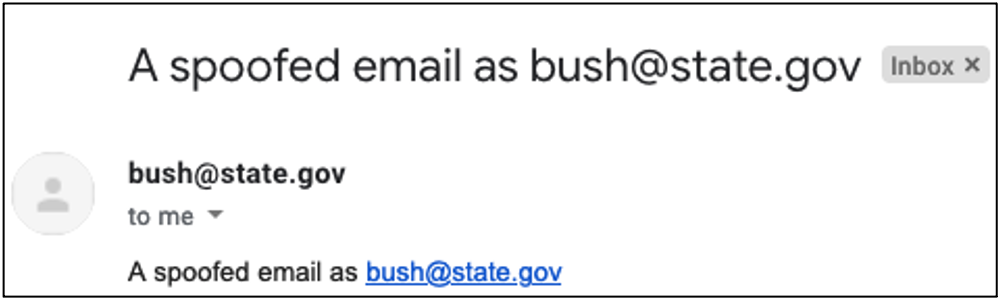
\includegraphics[width=\columnwidth]{graphs/ss_outlook_open_forwarding.png}}
{
    \setlength{\fboxsep}{0pt}
    \setlength{\fboxrule}{0.5pt}
    \fbox{
\includegraphics[width=\columnwidth]{graphs/ss_gmail_via_ui.png}}
}
%  \vspace*{-0.2in}
  \caption{Gmail annotating the sending address of an email. 
}
%\vspace*{-0.1in}
\label{fig:gmail_via}
\end{figure}

\subsection{Gmail UI Bug}
\label{subsec:ui_bug}
After a receiver accepts and processes email,
the user's mail user agent (MUA) displays the message for viewing.
Thus, MUAs and their UI warnings serve as the last line of defense against spoofed email messages.
However, previous work~\cite{hu_end--end_nodate,shen2020weak,chen2020composition} has found multiple security issues in various MUAs, especially on mobile platforms.
In our experiments, I focus on the native MUAs (web interfaces) provided by the nine email platforms in our study.
These MUAs not only have widespread usage, as the default MUA for many users,
but are also maintained by the email providers and tend to have better security practices.
% I focus on native MUAs because they tend to do their due diligence on the implementing a comprehensive UI warning system.

Among all native MUAs, only Gmail, Onet and Zoho have implemented warning
systems that display UI indicators when an email is forwarded or fails
DMARC authentication.  Gmail, for instance, annotates the
sending address (e.g., \dns{adminrec@univ.edu} \textit{via} \dns{e2ma.net} as shown in Figure~\ref{fig:gmail_via}).

%% Figure~\ref{fig:gmail_ui_normal} shows an example of Gmail displaying
%% a UI notice for a forwarded message (in this case via
%% \dns{gmail.com}).

However, I observed a bug in Gmail's warning system for a subset of forwarded
messages. In particular, Gmail does not display an indicator for a forwarded
email message if (1) it does not contain any DKIM headers, and (2) it has the
same domain in both the \textsc{MAIL FROM} and \textsc{FROM} headers.
%Figure~\ref{fig:gmail_ui_bug} shows an example of such an email message.
This policy does not pose a problem in single-sender email settings, because adversaries still need to bypass SPF and DMARC.
However, I present a new attack that uses this bug in conjunction with forwarding and other vulnerabilities to deliver spoofed email messages that look no
different than legitimate messages (Section~\ref{subsec:attack_relaxed_forwarding_validation}).
% \geoff{where in \ref{subsec:attack_relaxed_forwarding_validation}?}\alex{updated \ref{subsec:attack_relaxed_forwarding_validation}}
% \section{Mitigation}
% The attacks I demonstrate highlight the complicated interactions between email forwarding and existing anti-spoofing mechanisms.
% Below I propose several defenses that email platforms can use to mitigate each attack.
% While these defenses use existing and practical mechanisms, they often require changes by multiple or unaffected parties across the email ecosystem (e.g., changes by forwarding providers to protect downstream recipients).
% This quagmire underscores the complexity that email forwarding adds to anti-spoofing measures and illustrates the need for more holistic and comprehensive approaches to improving email security.

% To mitigate the first three attacks I demonstrate in this paper, I recommend all mail service providers disable \emph{open forwarding}, and instead require confirmation by the forwarding recipient as part of the process.
% Although this design will incur additional effort by every user who sets up forwarding, it will mitigate these three attacks, since all of them leverage the \emph{open forwarding} feature of email platforms.
% Additionally, I suggest that providers enforce rejection (outright dropping) of email messages that fall under the scope of a DMARC reject policy. Had Outlook rejected the spoofed email messages in the first place, the impact of the first attack (Section~\ref{subsec:attack_open_forwarding}) would narrow substantially.
% Unfortunately, both of these defenses reflect a case of misaligned
% %harms
% incentives: the recipients of spoofed email (\eg, spam and phishing) cannot implement this change,
% but instead need to rely on the entire ecosystem of providers and forwarding services to adopt such defenses.

% Email providers can mitigate the second attack (\S~\ref{subsec:attack_relaxed_forwarding_validation}) by eliminating the relaxed validation policies.
% This approach would protect their users from receiving spoofed email without relying on changes by other platforms or services.
% However, to ensure that benign forwarding does not break, providers will likely need to implement ARC validation, which requires forwarders from external services to implement it and potentially introduces new problems such as trust issues.
%  % Finally, while relaxed validation certainly helps increase the deliverability of forwarded email messages, I recommend implementing ARC and stick with DMARC policy when possible.

% For the final attack that abuses mailing lists, I suggest two different defenses that trade usability for security.
% % As for the attack on mailing lists, there exists two types of defense mechanisms that trade usability for security.
% First, list owners can turn on message moderation or set their mailing lists to be private.
% These measures increase the difficulty of performing email spoofing attacks,
% but do not rule out the attack entirely. A dedicated attacker might
% nonetheless identify a member of the mailing list and craft an email
% that fools a list's moderator.
% Second, some mailing list services, such as Listserv, support confirm-before-send~\cite{OnmyLIST7:online}, which requests confirmation from the (true) sender address before delivery.
% However, the additional overhead this imposes for each message might prevent widespread use.
% As a compromise, I recommend that mailing lists turn on this option by
% default for any incoming email that fails DMARC authentication checks.

% % While these short-term fixes will significantly reduce the exposure to the
% % attacks I have described here, I believe ultimately email requires a more
% % solid security footing if it is to effectively resist spoofing attacks going forwards.


\section{Additional Attack Screenshots}
% \paragraph{Additional Screenshots}
I ran a small set of experiments that spoofed email impersonating real domains to validate the attacks described in Section~\ref{sec:attacks}.
Our experiments confirmed that these attacks succeed.
Below, I present the screenshots of spoofed email messages successfully delivered to users' inboxes.

For the attack described in Section~\ref{subsec:attack_relaxed_forwarding_validation}, Figure~\ref{fig:ss_gmail_via_outlook} shows a spoofed message forwarded via a personal Outlook account to a Gmail account I created, and delivered to the recipient's inbox without any security warnings.
The spoofed address in this example impersonates a sender at \dns{alipay.com} (a prominent Chinese payment company with a DMARC policy of \textsc{Quarantine}).

For the attack described in Section~\ref{subsec:attack_zoho_arc}, Figure~\ref{fig:ss_zoho_arc} illustrates that this attack succeeds
without any security warnings, even though the spoofed domain in our
experiment, \dns{facebook.com}, has a DMARC policy of \textsc{Reject}.


% \paragraph{Additional Details for the Attack in Section~\ref{subsec:attack_relaxed_forwarding_validation}}
\section{Additional Details for the Attack in Section~\ref{subsec:attack_relaxed_forwarding_validation}}
\label{sec:append_change_behavior_details}
This section makes three additional observations about the attacks on
providers with relaxed forwarding validation as described in
Section~\ref{subsec:attack_relaxed_forwarding_validation}.

First, in addition to forwarding from personal Outlook accounts, an
adversary can also forward from personal accounts with other providers
(\eg, Fastmail) to Gmail recipients.
As mentioned earlier in Section~\ref{subsubsec:relaxed_validation}, there is an additional caveat: the \textsc{TO} header of the spoofed email cannot be the same as victim's email address.
An astute recipient might see that the \textsc{TO} field corresponds to someone else's email account, and become suspicious about the email's validity.
To reduce suspicion in this case, the adversary can set the
human-readable name portion of the email's \textsc{TO} header to
``me'' or the victim's name (while keeping the address different).

Second, adversaries need to leverage popular mail providers as forwarders in this attack; they cannot exploit relaxed forwarding validation by using their own servers as forwarders.
In our experiments, I tested using both a personal Outlook account as well as a mail server I controlled as forwarders.
The first version results in successful attacks delivered to user inboxes, but the latter did not.
I suspect this outcome is because our mail server domain has lower reputation than Outlook's mail servers.

Finally, in Section~\ref{subsec:attack_relaxed_forwarding_validation}, I demonstrate the attack against a recipient using Gmail. A similar attack can be mounted against Outlook recipients by
forwarding via a personal Fastmail account. This attack allows an
adversary to spoof email messages from many domains that have a DMARC
policy \textsc{None} to arbitrary Outlook recipients.\footnote{Similar to the caveats described in
Section~\ref{subsubsec:quarantine_instead_of_reject}, I observe that Outlook applies
additional restrictions to a small set of high-profile domains with a
DMARC policy of \textsc{None} (e.g., \dns{citizensbank.com}), which blocks the delivery of spoofed emails from these domains.}
Figure~\ref{fig:attack_none_ms} shows a spoofed email message
forwarded via a personal account to an Outlook account I created, and
delivered without any security warnings. The spoofed FROM header in
this example impersonates a sender at \dns{lesechos.fr} (a French
financial newspaper with a DMARC policy of \textsc{None}).

\begin{figure}[t]
  \centerline{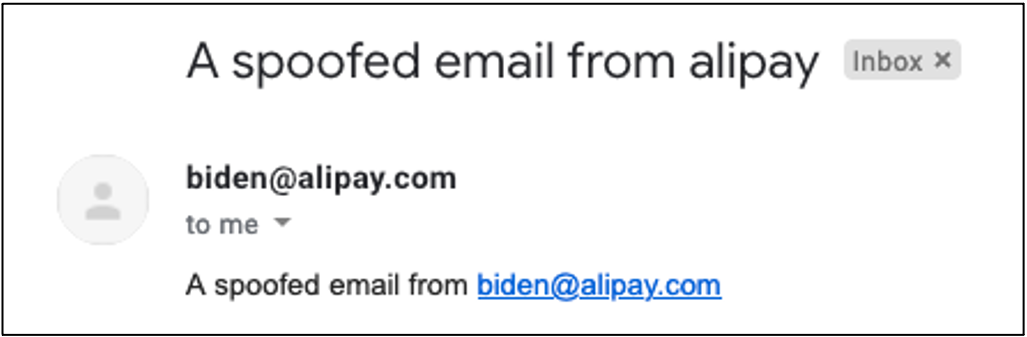
\includegraphics[width=\columnwidth]{graphs/ss_gmail_via_outlook.png}}
  \centering
  \caption{Email spoofing \dns{biden@alipay.com} via Outlook.}
  \label{fig:ss_gmail_via_outlook}
  \end{figure}


\begin{figure}[t]
  \centerline{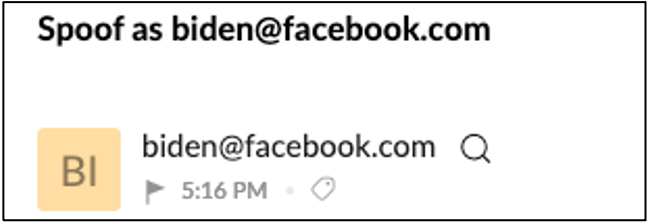
\includegraphics[width=\columnwidth]{graphs/ss_zoho_arc.png}}
  \centering
  \caption{Email spoofing \dns{biden@facebook.com} via Fastmail.}
  \label{fig:ss_zoho_arc}
  \end{figure}

\begin{figure}[t]
\centerline{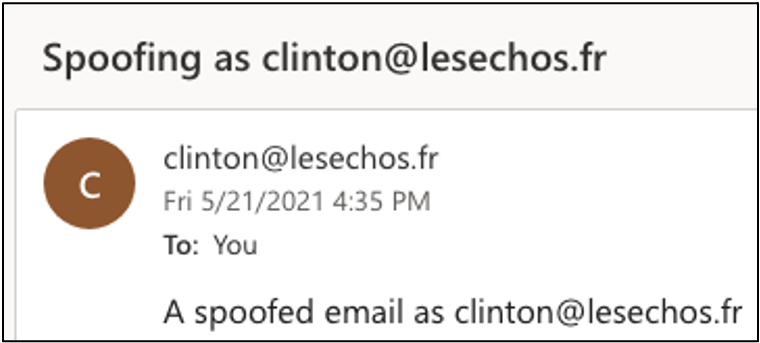
\includegraphics[width=\columnwidth]{graphs/ss_outlook_none.png}}
\centering
\caption{Spoofed email message taking advantage of Outlook's relaxed forwarding validation policy.}
% \geoff{let's see if Stefan notices this screenshot}}
\label{fig:attack_none_ms}
\end{figure}


\section{Additional Details for the Attack in Section~\ref{subsec:attack_zoho_arc}}
\label{sec:appendix_zoho_attack_details}
% \paragraph{Additional Details for the Attack in Section~\ref{subsec:attack_zoho_arc}}
Adversaries can broaden the scope of the attack described in Section~\ref{subsec:attack_zoho_arc} by using a forwarding
account at any email provider that Zoho trusts for ARC purposes,
including Gmail, and routing their spoofed email through multiple forwarding hops.
In particular, an attacker can obtain ARC headers in one forwarding hop via Gmail, and then bypass Gmail's lack of open forwarding by forwarding the email through a second account that does allow open forwarding (\eg, Outlook).
% The attacker can use a Gmail
% account to obtain the necessary ARC headers by including this account as an additional forwarding hop.
% For example, the attacker could create a second
% forwarding account on a platform that has open forwarding (\eg,
% Outlook).
For example, first, the attacker would send their spoofed email message
to their Gmail account, which they configured to forward to their
malicious Outlook account.
During the forwarding process Gmail will
attach a set of ARC headers to the email message.
Next, the spoofed email will arrive at their malicious Outlook account, which then forwards the email to any arbitrary Zoho recipient (because Outlook
supports open forwarding).
This forwarded email message will contain Gmail's attached ARC headers, enabling the attack to successfully pass DMARC validation checks as a result of Zoho's vulnerable ARC implementation.

Using our test accounts, I validated that this multi-hop attack variation
successfully delivers spoofed messages to the inbox of a Zoho recipient
without any warnings.






\section{Additional Details for the Attack in Section~\ref{subsec:attack_none_mailing_list}}
% \paragraph{Additional Details for the Attack in Section~\ref{subsec:attack_none_mailing_list}}
\label{sec:append_mailing_list_details}

% \subsection{Abusing Gaggle.email}

\begin{figure}[t]
\centering
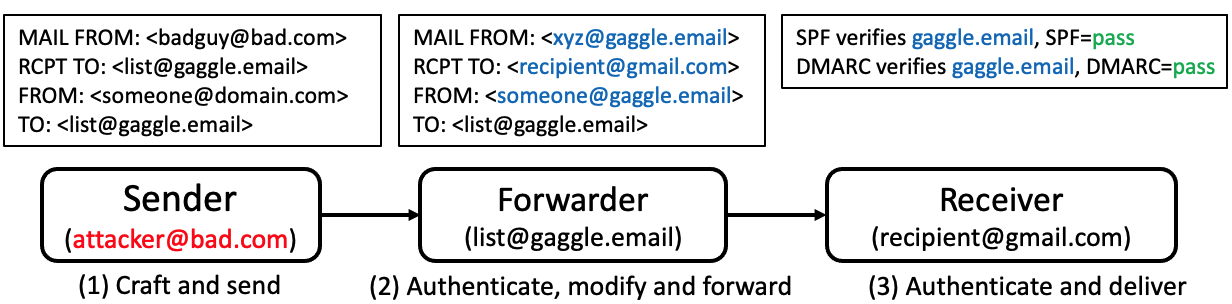
\includegraphics[width=\columnwidth]{graphs/mech_gaggle.png}
\centering
\caption{Attack flow for Gaggle.}
\label{fig:gaggle_email_mech}
\end{figure}

In addition to the attacks described in
Section~\ref{subsec:attack_none_mailing_list}, I found
additional attack variants related to Gaggle.
Figure~\ref{fig:gaggle_email_mech} shows an example of an attack that
abuses Gaggle's use of REM + MOD forwarding
(Section~\ref{sec:measure_forwarding_mechs_and_arc}). This attack works
regardless of the DMARC policy of the spoofed address's domain.  First, an
attacker chooses an address to spoof (\dns{someone@foo.com}) that is
allowed to send to a mailing list on a vulnerable provider
(\dns{list@gaggle.email}), and sends a spoofed email message
purporting to come from that address.  This spoofed email will fail
DMARC validation, but because Gaggle does not enforce DMARC
(Appendix~\ref{subsec:no_dmarc}), it will forward the email to the
mailing list's recipients as normal (Stage 2).  Since Gaggle uses a
REM + MOD forwarding process, it will rewrite the \textsc{MAIL FROM}
header to use the mailing list's domain (\eg, a
new \textsc{MAIL FROM} address of \dns{xyz@gaggle.email}).
%\grant{Similar to earlier, I should be more precise.}
Finally, when the spoofed email message arrives at the recipient's mail server,
it will properly pass SPF validation and DMARC alignment checks:
the rewritten \textsc{MAIL FROM} domain allows the mailing list to send on its behalf, and the domain matches the \textsc{FROM} address's domain (\dns{gaggle.email}).

% \subsection{Other Details}
% Below, I note one additional detail\alex{fix this number} about this attack.

Additionally, I note that mailing list software such as Listserv and
Mailman require a backend MTA.  In our experiments I used Postfix
with DMARC turned on, a configuration which follows good security
practice.  However, in practice many organizations might not use this
configuration because many MTAs (including Postfix) do not enforce
DMARC by default.  In these cases, the attacker can spoof email from any
target domain, regardless of its DMARC policy, much like the attack
against Gaggle.


%\section{Limitations}
%Most of the attacks described in this paper require that the attacker has an account on an email forwarding service and can configure the account to forward email message to the target account. Thus, massively and automatically performing the attacks described in this paper can be challenging. Automating the attacks (e.g., via automated account creation) is out of scope for this work.




%%%%%%%%%%%%%%%%%%%%%%%%%%%%%%%%%%%%%%%%%%%%%%%%%%%%%%%%%%%%%%%%%%%%%%%%%%%%%%%%
\end{document}
%%%%%%%%%%%%%%%%%%%%%%%%%%%%%%%%%%%%%%%%%%%%%%%%%%%%%%%%%%%%%%%%%%%%%%%%%%%%%%%%

%%  LocalWords:  endnotes includegraphics fread ptr nobj noindent
%%  LocalWords:  pdflatex acks
